\documentclass[letterpaper,12pt]{report} % Set paper size to US Letter
\usepackage{graphicx}   % For including images
\usepackage{amsmath}    % For mathematical expressions
\usepackage{amssymb}    % Additional math symbols
\usepackage{booktabs}   % For professional-looking tables
\usepackage{float}      % For precise placement of figures/tables
\usepackage{hyperref}   % For clickable links
% \usepackage{geometry}   % Page layout customization
\usepackage{enumitem}   % Customizable lists
\usepackage{fancyhdr}   % For headers and footers
\usepackage{titlesec}   % Section title formatting
% \usepackage[numbers]{natbib} % Use natbib for ASCE-like citation style
\usepackage{makecell}
\usepackage{tabularx}
\usepackage{multirow}
\usepackage{booktabs}
\usepackage{adjustbox}
\usepackage{array}
\usepackage{pdfpages}   % to include external PDFs
\usepackage{caption}    % for \captionof if you want LoF entries
\usepackage[T1]{fontenc} % Recommended for better font handling
\usepackage{url}
\urlstyle{same} % This makes URLs use the same font as the main body text

\usepackage{chngcntr}



% ---------- Bibliography ----------
\usepackage[
    backend=biber,
    style=ieee,
    sorting=none,
    giveninits=true,
    maxnames=6,
    doi=false,
    isbn=false,
    url=true
]{biblatex}

\addbibresource{references.bib} % your .bib file


\usepackage{tikz}
\usetikzlibrary{arrows.meta, positioning, shapes.geometric}

\usepackage[margin=1in]{geometry}
\usepackage{setspace}
% \usepackage{ulem} % for underline
\usepackage[normalem]{ulem}   % keep \emph as italics; avoids biblatex clash



\usepackage{amsfonts}
\geometry{letterpaper, margin=1in} % Set margin for US Letter paper
\setlength{\parindent}{0pt}    % No indentation
\setlength{\parskip}{1em}      % Add one line of vertical space between paragraphs
\newcolumntype{Y}{>{\centering\arraybackslash}X}  % centered X column

% Change TOC, List of Figures, and List of Tables titles
\renewcommand{\contentsname}{Table of Contents}
\renewcommand{\listfigurename}{List of Figures}
\renewcommand{\listtablename}{List of Tables}

% Use ASCE-like bibliography style
% \bibliographystyle{unsrt} % unsrt provides ASCE-like numbered citations

% Title Page
% \title{\textbf{Sanitary Pump Selection and Force Main Design for Colebrooke Subdivision}}
% \date{}

\doublespacing
\begin{document}

\begin{titlepage}
    \begin{center}
        % University Logo (Placeholder)
        \vspace*{-2cm}
        
\includegraphics[width=0.3\textwidth]{JSUmanualPg39.jpg} % Replace with actual file name
        \vfill


        % Course Name and Experiment Title
        {\Large \textbf{CIV410 - Capstone Design I}}\\[0.6cm]
        {\Huge \textbf{Final Design Report on Colebrooke Subdivision Pump Selection and Force Main}}\\[1.5cm]

        % Instructor Information
        \textbf{Instructor:} Kejun Wen, PhD \\[1.5cm]

        % Student and Group Information
        \textbf{Prepared by:} \\[0.2cm]
        {\Large Shams E Shifat (J01033311)}

        {\large Group 2 | Nova Build Collective}\\[1cm] % Increased spacing here


        % Experiment and Submission Dates
        \textbf{Date of Submission:} \today \\[2cm]
        \vfill
    \end{center}
\end{titlepage}


\chapter*{Executive Summary}
\addcontentsline{toc}{chapter}{Executive Summary}

This report presents the design and cost evaluation of a wastewater conveyance system for the proposed Colebrooke Subdivision located in Florence, Mississippi. Due to site topography, gravity flow alone is insufficient to transport wastewater to the existing municipal sewer system. As a result, a lift station and force main system were required to overcome elevation constraints and ensure reliable wastewater conveyance.

Three design alternatives were evaluated, including a centralized duplex pump station with force main, a distributed grinder pump system, and a deep gravity sewer system. Based on hydraulic performance, constructability, cost, operational reliability, and long-term maintenance considerations, the duplex submersible pump station with a pressurized force main was selected as the most appropriate solution. This configuration provides a balance of reliability, efficiency, and compliance with applicable design standards, including MDEQ and Ten States guidelines.

The final system consists of a duplex submersible pump station discharging through a 4-in PVC force main extending 77.48~ft to an existing municipal sewer manhole. The design is governed by a peak wastewater inflow of 12.46~gpm and a static head of 10.28~ft. The selected pump, Sulzer XFP100C VX, operates at 135.5~gpm and 12.08~ft of head, ensuring adequate capacity and solids-handling capability. The wet well is designed as a 6-ft diameter structure with 250~gal of active storage, providing stable pump cycling and operational reliability.

Hydraulic analysis confirmed that the selected force main and pump configuration satisfy velocity, headloss, and performance requirements. The system achieves a flow velocity of approximately 3.4~ft/s, exceeding the minimum self-cleansing velocity while maintaining efficient operation. The duplex configuration provides redundancy, ensuring continuous service during maintenance or pump failure.

A comprehensive cost estimate was developed using regional bid data, standard cost references, and vendor-based pricing. Direct construction costs total \$210{,}062.44, with additional indirect, engineering, and contractor-related costs resulting in a total project cost of \$323{,}817.42. The analysis indicates that the lift station structure, electrical and control systems, and excavation work dominate the overall cost, while the force main represents a relatively small portion of the budget.

Overall, the proposed design provides a practical, reliable, and cost-effective solution for wastewater conveyance within the Colebrooke Subdivision. The system satisfies hydraulic and regulatory requirements, supports long-term municipal operation, and establishes a robust foundation for future development and infrastructure integration.
% This report presents the preliminary design and evaluation of a wastewater conveyance system for the proposed Colebrooke Subdivision in Florence, Mississippi. The project was undertaken to develop a reliable and cost-effective solution for collecting and conveying domestic wastewater from thirteen residential lots to the downstream municipal system. The work included analysis of site conditions, estimation of design flows, evaluation of system alternatives, and preparation of preliminary cost estimates in accordance with Mississippi Department of Environmental Quality (MDEQ) guidance~\cite{MDEQ_DesignGuidance_2025}.

% Based on population projections and standard design assumptions, the peak design flow was determined to be approximately 19~gallons per~minute (gpm). Three alternatives were considered: (1) a duplex submersible pump station with a PVC force main, (2) a grinder pump and low-pressure sewer system, and (3) a deep gravity sewer. After technical, economic, and operational evaluation, the duplex submersible pump station with a 4-in PVC C900 DR18 force main was selected as the preferred option. This configuration provides dependable performance, simplified maintenance, and long-term sustainability for small residential developments.

% The total estimated construction cost for the selected design is approximately \$404{,}375, with an annual operation and maintenance cost of about \$7{,}500. The design achieves a balanced approach between performance, cost, and reliability while maintaining compliance with all applicable standards. Overall, the results demonstrate that the selected system is both technically sound and economically viable, forming a strong foundation for final design development and implementation in the next phase of the project.




\newpage
\tableofcontents   % Generates TOC
\newpage
\listoffigures
\newpage
\listoftables
\newpage


% \maketitle

% \begin{center}
%   {\LARGE \textbf{Sanitary Pump Selection and Force Main Design for Colebrooke Subdivision}}
% \end{center}
% \hrule


% Include separate section files
% \input{sections/part1.tex}
% \newpage
% \input{sections/part2.tex}
% \newpage
% \input{sections/part3.tex}
% \newpage
% \input{sections/part4.tex}
% \newpage
% \input{sections/part5.tex}
% \newpage
% \input{sections/part6.tex}

\chapter{Introduction}
\section{Project Background}

The Colebrooke Subdivision is a proposed residential development located in the City of Florence, Rankin County, Mississippi, approximately 1{,}825~ft west of Seventh Day Road on the north side of Lewis Street~\cite{ProjectD_Colebrooke_2020}. The site consists of previously undeveloped land characterized by gently rolling terrain and surrounding residential and semi-urban land uses. The development is part of ongoing regional growth and is intended to expand residential capacity while providing essential infrastructure to support future occupants.

The project involves the preparation of a comprehensive civil engineering design to establish the infrastructure required for a functional residential community. These infrastructure components include roadway systems, stormwater management facilities, and a sanitary sewer network designed to safely collect and convey wastewater generated by the subdivision to the existing municipal sewer system. The preliminary subdivision layout defines internal road alignments, lot configurations, and utility corridors in accordance with municipal planning requirements and design standards~\cite{ProjectD_Colebrooke_2020}.

\begin{figure}[H]
    \centering
    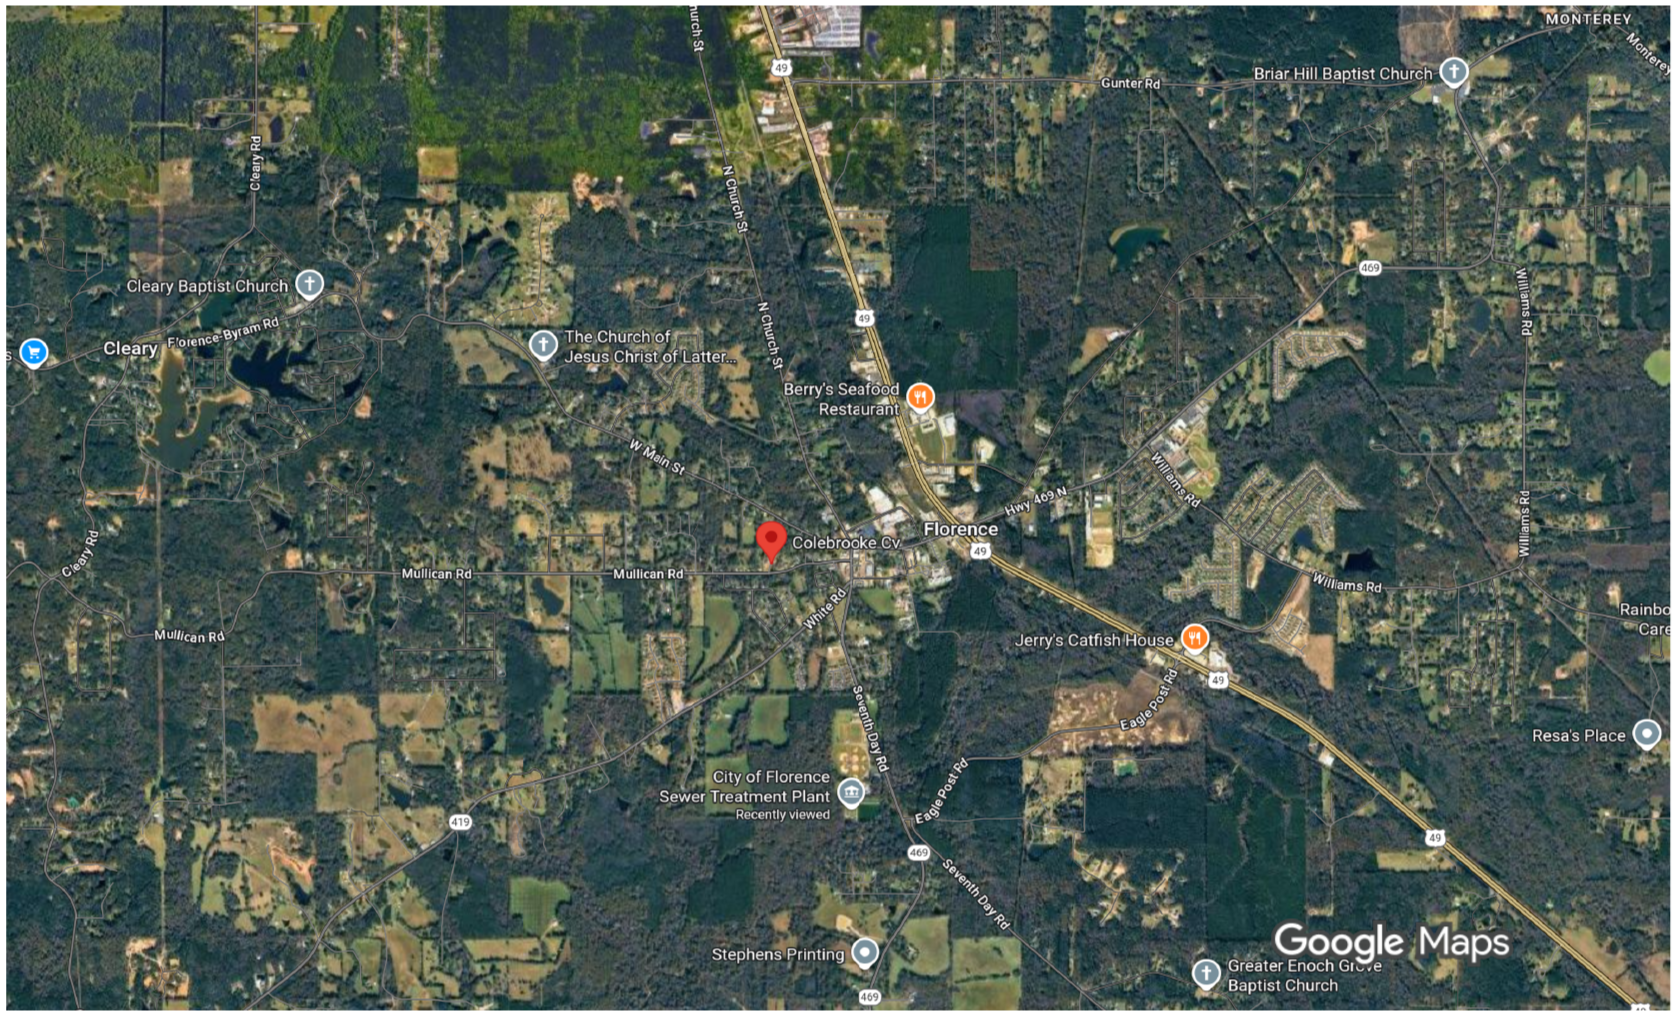
\includegraphics[width=0.76\textwidth]{figures/site.png}
    \caption{Colebrooke Subdivision Location Map.}
    \label{fig:colebrooke_location}
\end{figure}

The infrastructure systems within the subdivision are designed to operate as an integrated network that supports long-term functionality, environmental protection, and public health. Within this network, the sanitary sewer system plays a critical role by ensuring the reliable collection and transport of domestic wastewater. The performance of this system is essential for maintaining safe living conditions and preventing environmental contamination, making it a key component of the overall subdivision design.


\section{Need for a Pump Station}

The sanitary sewer system proposed for the Colebrooke Subdivision is designed to collect wastewater from individual residential lots through a gravity-driven network and convey it to the existing municipal sewer system. Under ideal conditions, gravity flow provides a reliable and energy-efficient means of wastewater transport. However, the topographic characteristics of the project site impose a fundamental limitation on the use of a gravity-only system.

The gently rolling terrain of the subdivision results in a local low point within the development where wastewater accumulates. The elevation of this low point is insufficient to allow continuous gravity discharge to the downstream municipal sewer connection. As a result, wastewater cannot be conveyed entirely by gravity without risking surcharge conditions, reduced hydraulic performance, or system failure.

To overcome this elevation constraint, a pump station and pressure force main are required to lift wastewater from the subdivision’s low point and convey it to the downstream municipal sewer system. The pump station provides the hydraulic energy necessary to overcome both the static elevation difference and the frictional losses within the force main, thereby ensuring continuous and controlled wastewater transport.

The pump station and force main therefore serve as a critical interface between the internal gravity sewer network and the external municipal system. The reliability of this subsystem is essential for maintaining uninterrupted wastewater conveyance, preventing system backups, and protecting public health and the surrounding environment. Consequently, the design must ensure adequate hydraulic capacity, operational redundancy, and compliance with applicable wastewater design standards, including the \textit{Guidance for the Design of Publicly Owned Wastewater Facilities} issued by the Mississippi Department of Environmental Quality (MDEQ) and the \textit{Recommended Standards for Wastewater Facilities} (Ten States Standards)~\cite{MDEQ_DesignGuidance_2025,TenStates_RecommendedStandards_2014}.

Figures~\ref{fig:colebrooke_aerial} and \ref{fig:colebrooke_plat} illustrate the project area and subdivision layout, highlighting the spatial configuration that necessitates the use of a pumping system.

\begin{figure}[H]
    \centering
    \includegraphics[page=2,angle=270,width=\textwidth]{./As-Bulids (1).pdf}
    \caption{Aerial View of the Project Area.}
    \label{fig:colebrooke_aerial}
\end{figure}

\begin{figure}[H]
    \centering
    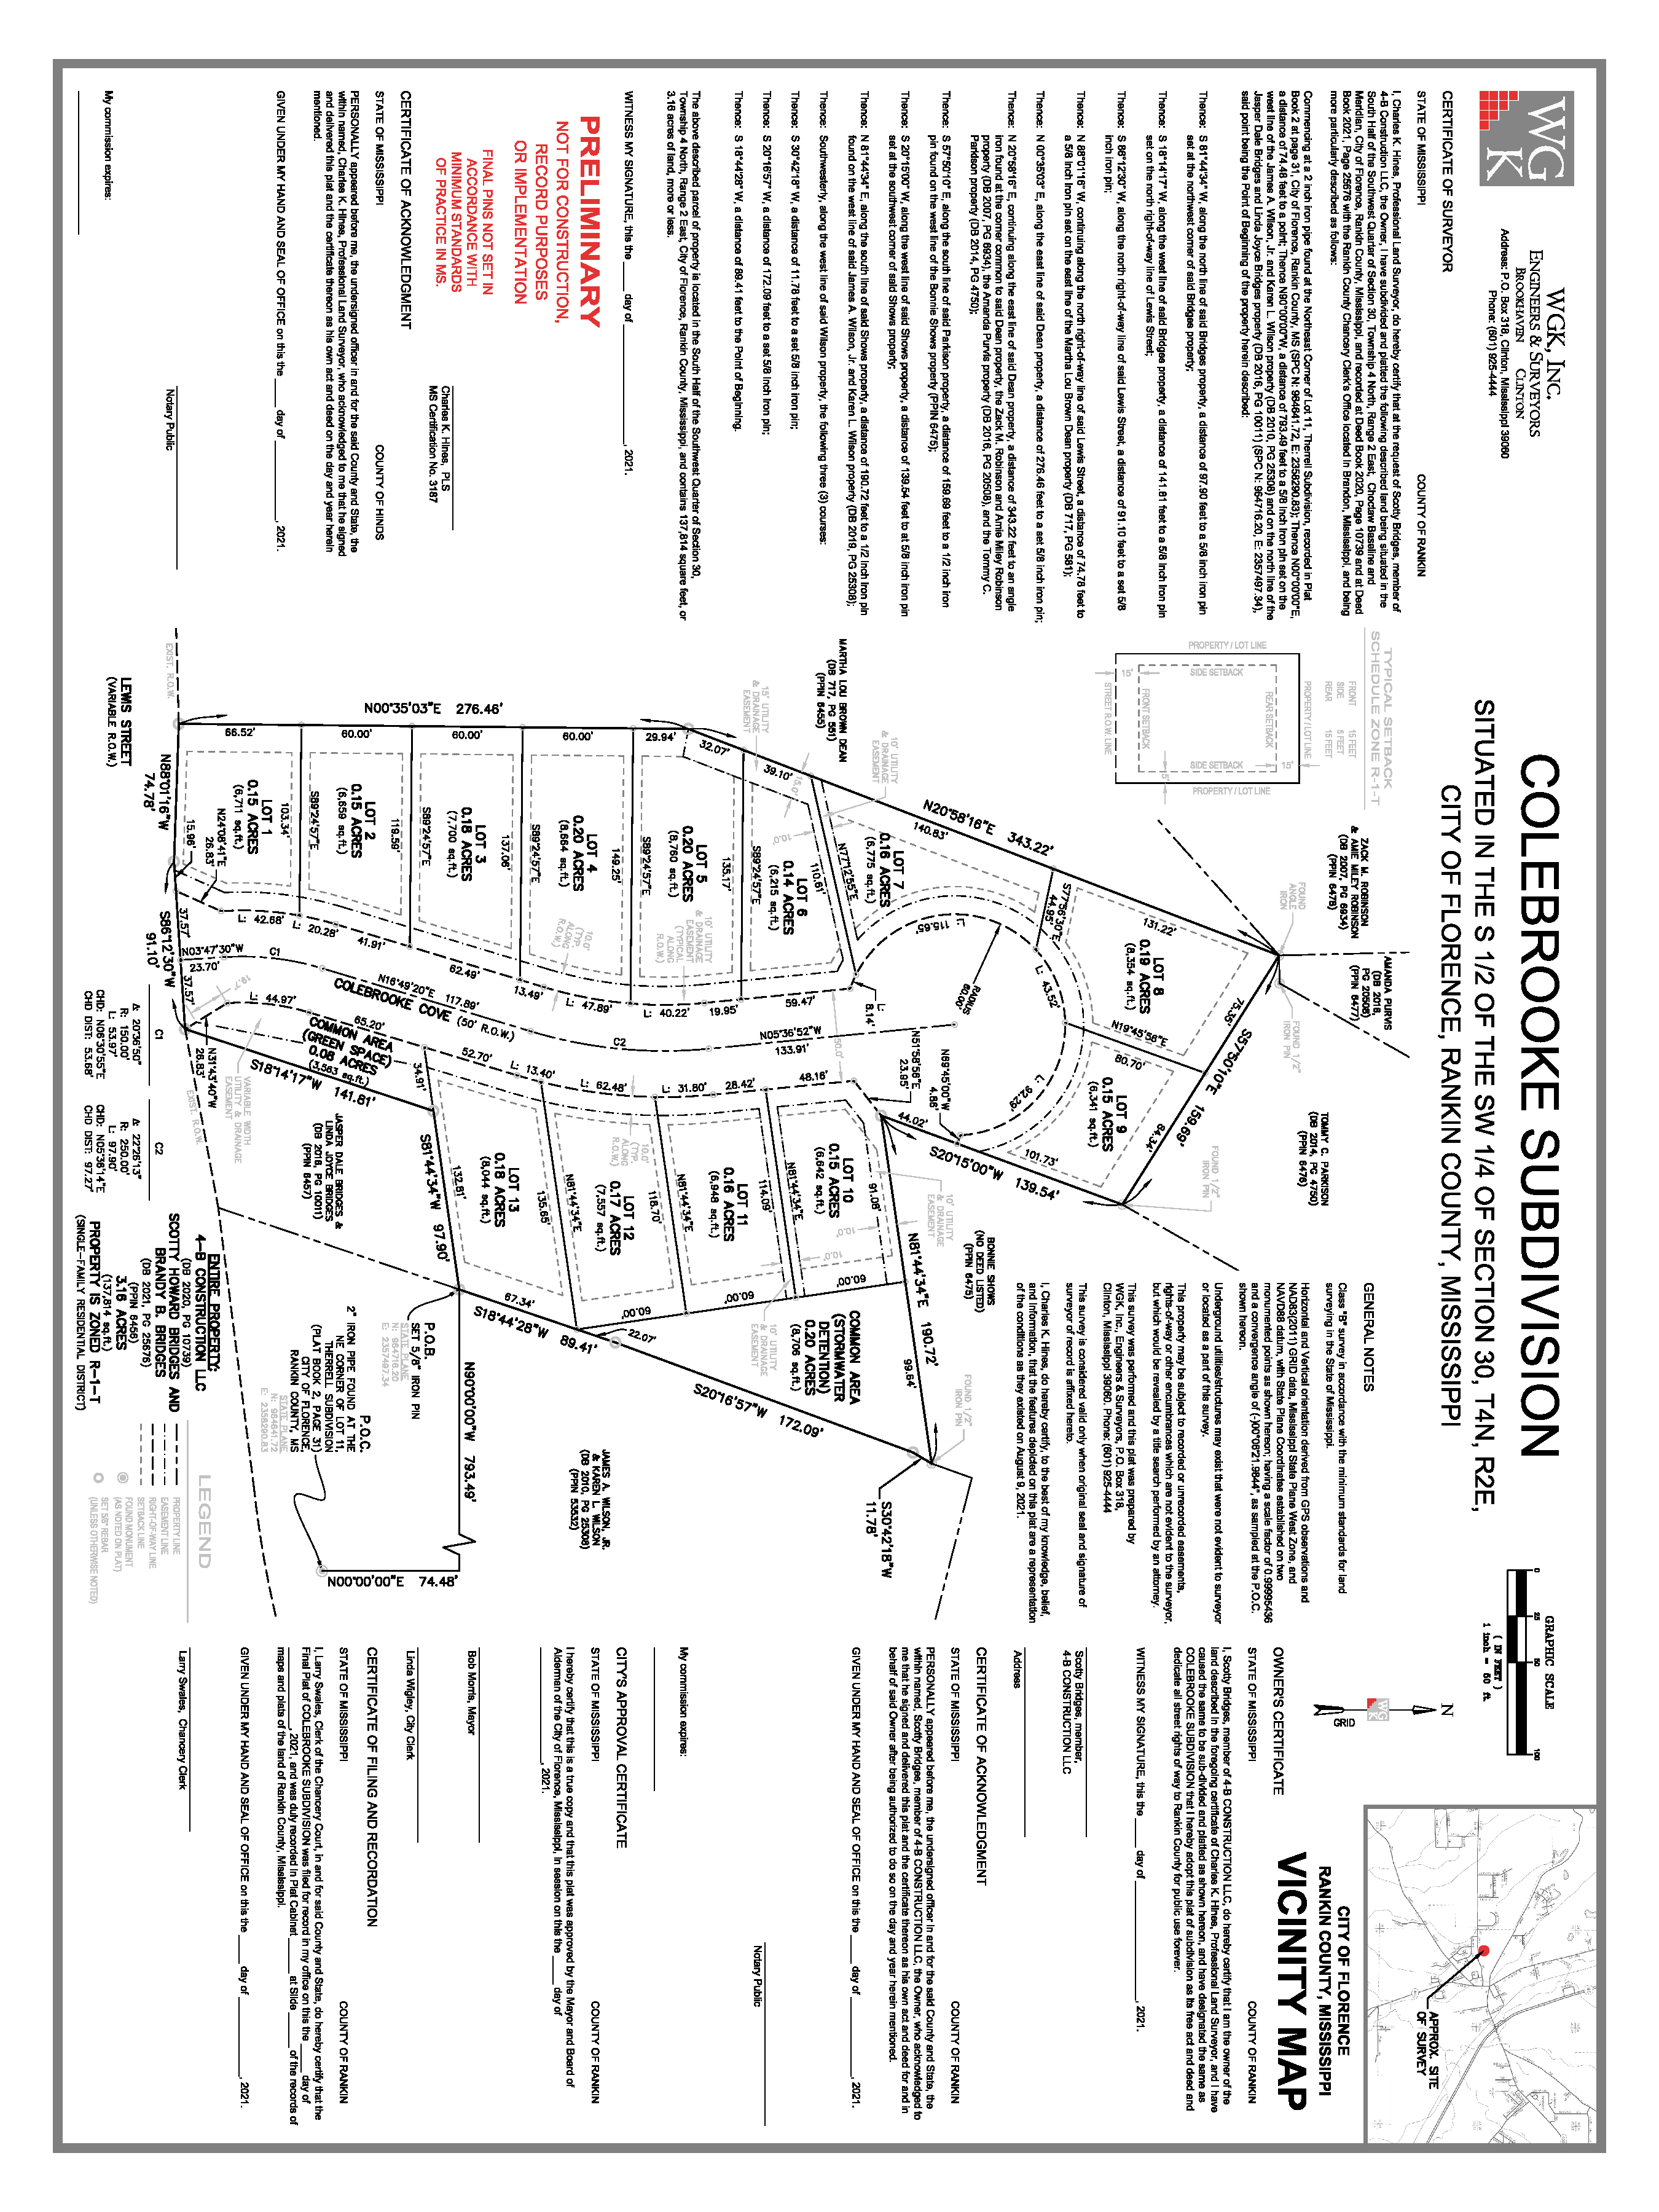
\includegraphics[angle=90,width=\textwidth]{./subdivision_plat_Prelim Plat_Colebrooke Subdivsion (1) (1).pdf}
    \caption{Preliminary Plat of the Colebrooke Subdivision.}
    \label{fig:colebrooke_plat}
\end{figure}



\section{Individual Design Scope and Objectives}

As the author of this report, I, Shams E. Shifat, was responsible for the design and evaluation of the pump station and force main subsystem within the Colebrooke Subdivision sanitary sewer network. This subsystem serves as the critical link between the subdivision’s internal gravity sewer system and the existing municipal sewer network.

My work focused on developing a design that satisfies the hydraulic, operational, and regulatory requirements of the system while accounting for site-specific constraints. The primary tasks included hydraulic analysis of the wastewater conveyance system, sizing and alignment of the force main, and selection of an appropriate pump configuration capable of meeting the system demand.

The design objectives were to ensure reliable wastewater conveyance under peak flow conditions, maintain self-cleansing velocities of at least 2~ft/s within the force main, and provide operational redundancy through a duplex pump configuration. Additional objectives included minimizing headloss within the system, optimizing energy efficiency, and selecting durable, corrosion-resistant materials suitable for long-term service.

The design was developed in accordance with the \textit{Guidance for the Design of Publicly Owned Wastewater Facilities} issued by the Mississippi Department of Environmental Quality (MDEQ) and the \textit{Recommended Standards for Wastewater Facilities} (Ten States Standards)~\cite{MDEQ_DesignGuidance_2025,TenStates_RecommendedStandards_2014}. The resulting design provides a practical and efficient solution for wastewater conveyance within the proposed residential development.


\section{Design Constraints and Assumptions}

The design of the pump station and force main system is governed by a combination of physical site conditions, regulatory requirements, and operational considerations. These constraints define the boundaries within which the hydraulic and structural design must be developed.

A primary physical constraint is the limited elevation difference between the subdivision and the downstream municipal sewer connection, which makes gravity-only wastewater conveyance infeasible. This condition necessitates the inclusion of a pump station to provide the hydraulic head required for wastewater transport. In addition, the site is underlain by moisture-sensitive silty clay soils, which require careful consideration for excavation stability, pipe bedding, and structural support of underground components.

Regulatory constraints are imposed by applicable wastewater design standards, including the \textit{Guidance for the Design of Publicly Owned Wastewater Facilities} issued by the Mississippi Department of Environmental Quality (MDEQ) and the \textit{Recommended Standards for Wastewater Facilities} (Ten States Standards)~\cite{MDEQ_DesignGuidance_2025,TenStates_RecommendedStandards_2014}. These standards establish requirements for system reliability, minimum flow velocity, pump redundancy, and wet well operation.

Operational considerations also influence the design. The system is intended to function under typical residential loading conditions and must ensure continuous and reliable wastewater conveyance. A duplex pump configuration is assumed to provide redundancy, allowing alternating operation and maintaining service during maintenance or equipment failure. The force main is designed to maintain self-cleansing velocities to prevent solids deposition and ensure long-term operational efficiency.

These constraints and assumptions provide the framework for the hydraulic analysis and design decisions presented in the subsequent chapters.

\newpage
\chapter{Site Conditions and Design Inputs}
\section{Site Description and System Layout}

The Colebrooke Subdivision is located in the City of Florence, Rankin County, Mississippi, and consists of a planned residential development situated along the north side of Lewis Street. The site is characterized by gently rolling terrain and has been subdivided into residential lots connected by internal roadways and utility corridors as defined in the preliminary subdivision plat~\cite{ProjectD_Colebrooke_2020}. 

The sanitary sewer system within the subdivision is designed as a gravity collection network that conveys wastewater from individual residential lots toward a designated low point within the site. Due to the site’s topography, wastewater cannot be discharged directly to the municipal sewer system by gravity alone. As a result, a pump station is located at this low point to collect and lift the wastewater for conveyance to the downstream municipal connection.

The pump station serves as the transition point between the internal gravity sewer system and the external pressurized conveyance system. From the pump station, wastewater is transported through a short force main that connects to an existing municipal sewer manhole located along Lewis Street. The force main alignment follows the shortest practical route between the pump station and the downstream connection point to minimize pipe length and hydraulic losses.

The overall configuration of the system, including the subdivision layout, gravity sewer alignment, pump station location, and force main connection, is illustrated in Figure~\ref{fig:pump_layout}. The figure identifies the spatial relationship between system components and establishes the geometric framework that governs the hydraulic design presented in subsequent sections.

\begin{figure}[H]
\centering
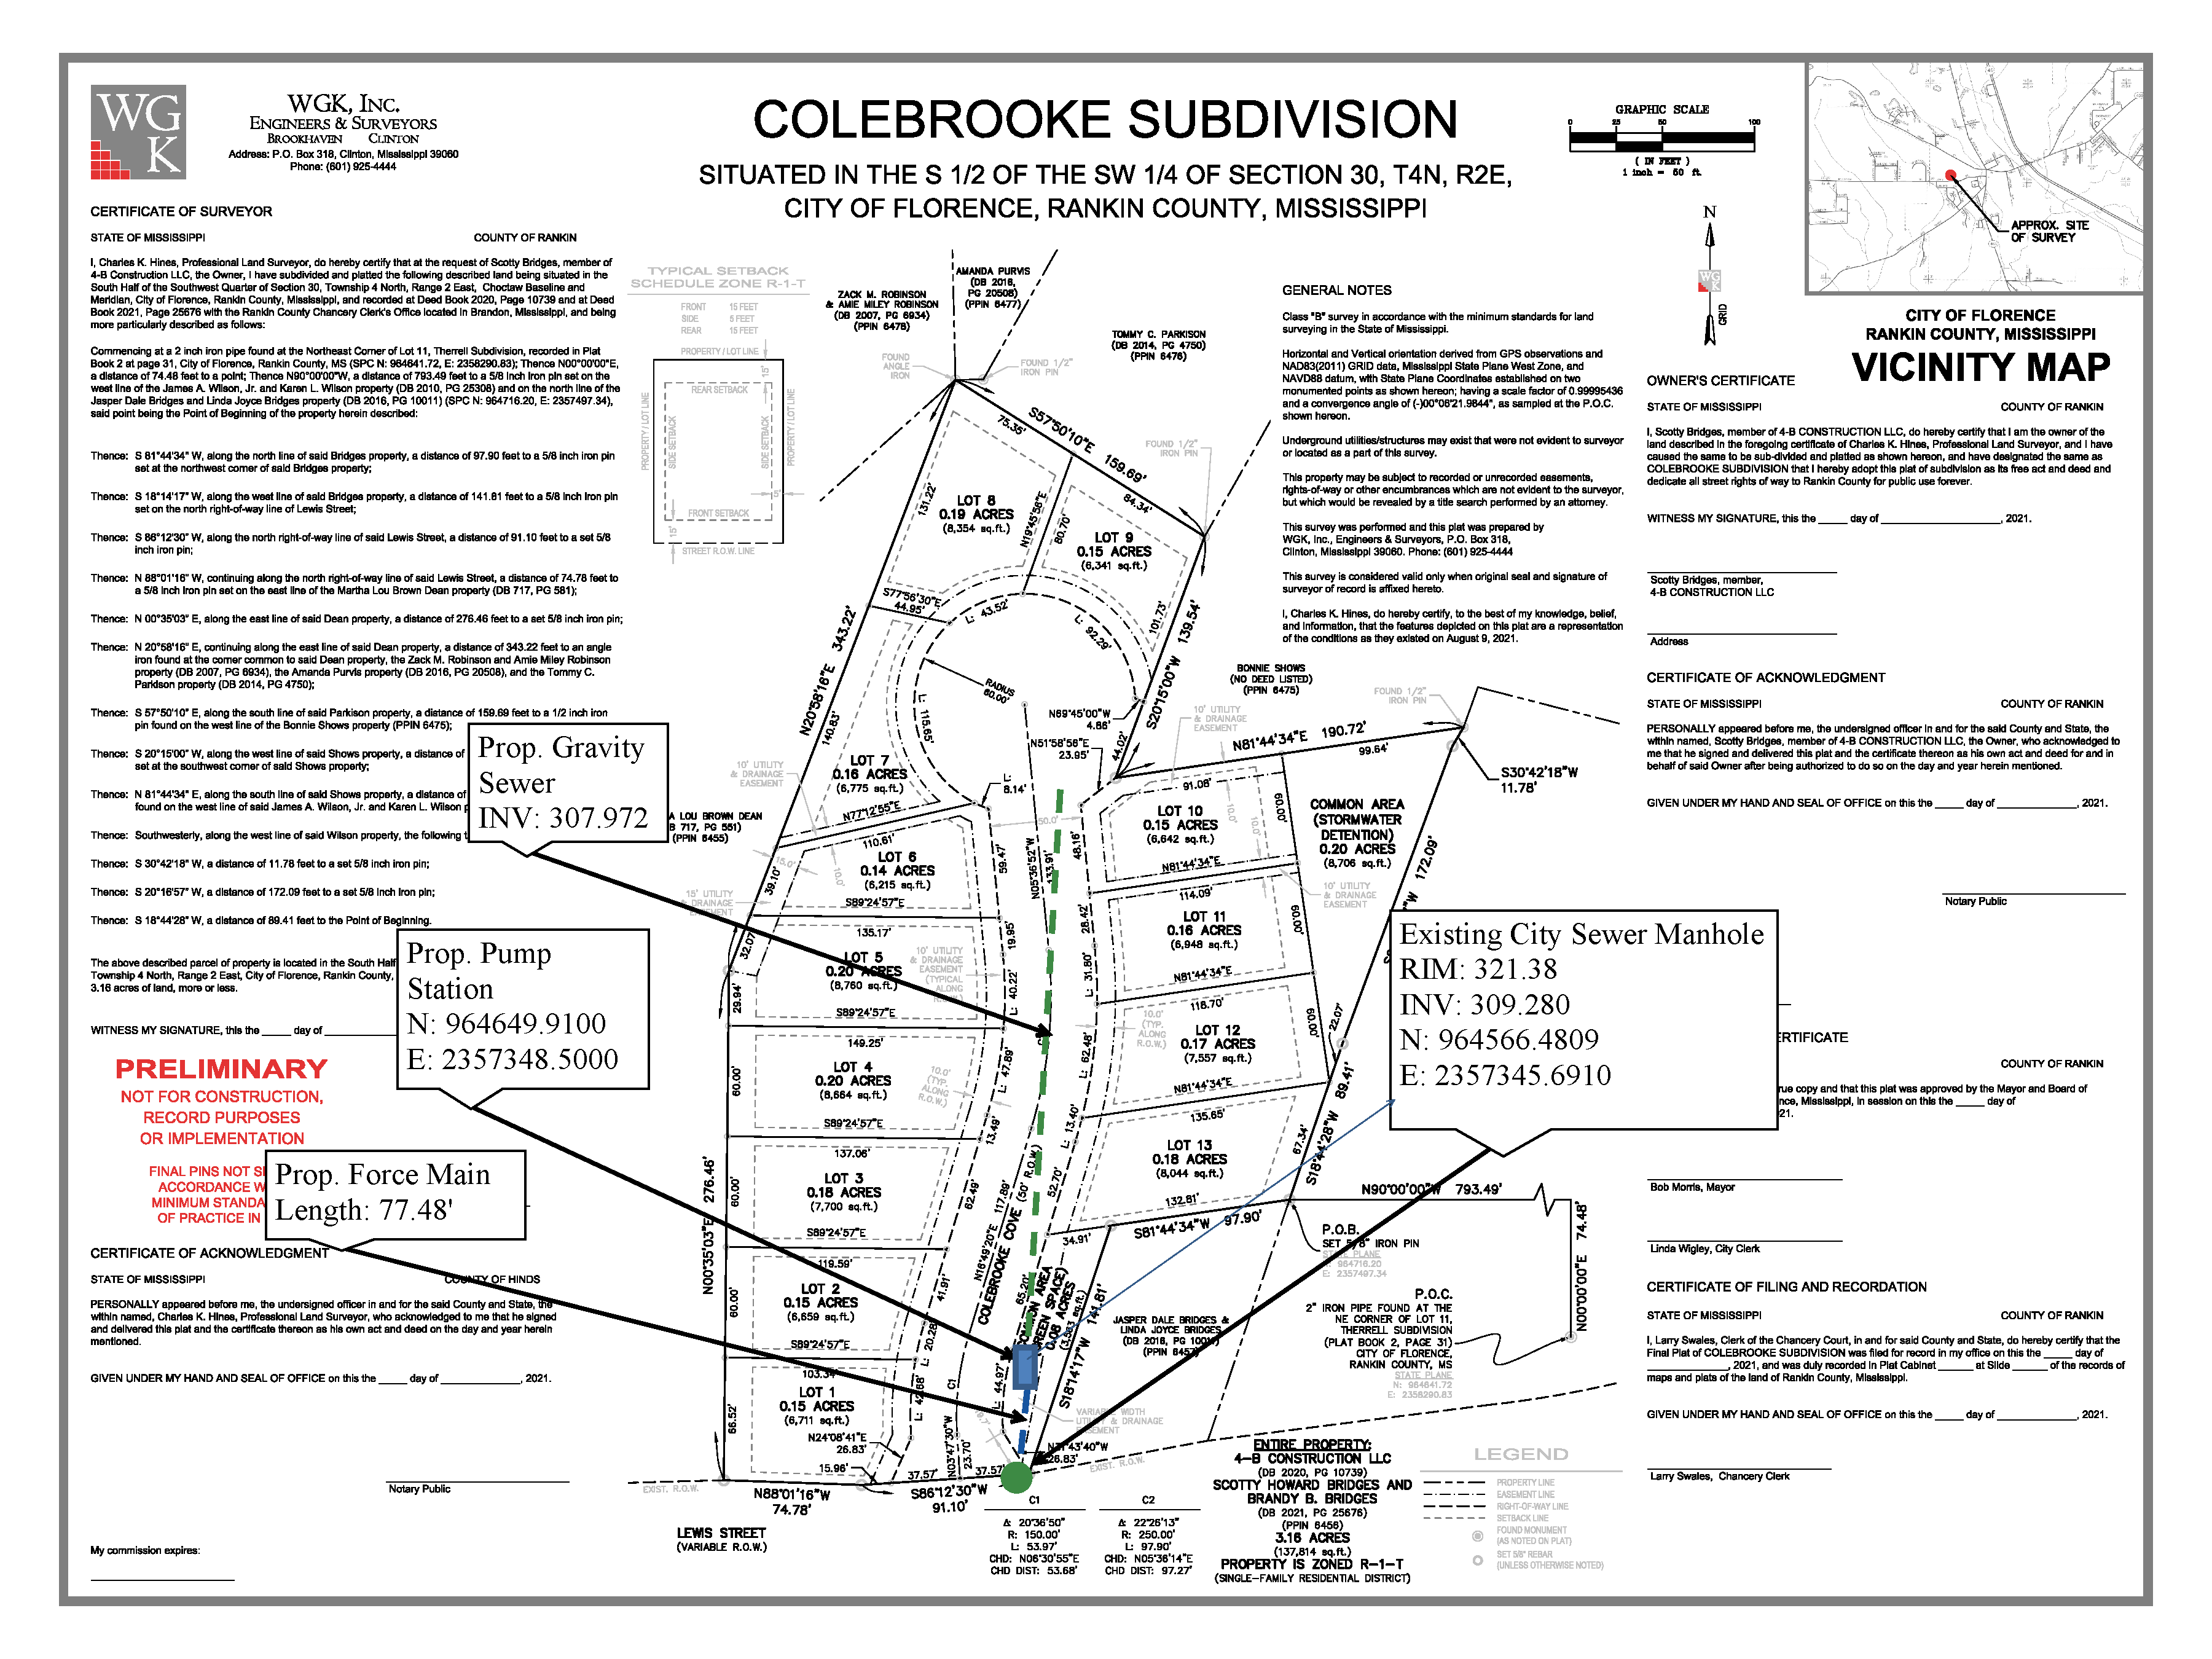
\includegraphics[width=\textwidth]{proposed_placement_plan_survey.pdf}
\caption{Proposed pump station location, gravity sewer alignment, and force main connection to existing municipal sewer manhole.}
\label{fig:pump_layout}
\end{figure}


\section{Wastewater Characteristics}

The conveyance system for the Colebrooke Subdivision is designed to transport domestic wastewater generated by residential units within the development. Unlike stormwater systems, which primarily convey runoff from precipitation events, sanitary sewer systems must handle wastewater containing suspended solids, organic matter, and other constituents typical of residential sewage.

The presence of suspended solids in wastewater introduces specific operational requirements for the conveyance system. In particular, the system must be capable of transporting solids without deposition, blockage, or excessive maintenance. This requirement influences both the hydraulic design of the force main and the selection of appropriate pumping equipment.

Wastewater lift stations are commonly equipped with submersible sewage pumps designed to operate under submerged conditions and convey both liquid and entrained solids. For residential wastewater applications, pumps are typically selected to accommodate the passage of solids of a specified size to ensure reliable operation. In this study, the system is assumed to handle solids up to approximately 3~inches in diameter, which is consistent with typical residential wastewater characteristics and standard pump capabilities.

These wastewater characteristics establish the functional requirements for the pump station and force main system, particularly with respect to maintaining adequate flow conditions and ensuring reliable transport of solids through the conveyance system.



\section{Design Flow and System Inputs}

The hydraulic capacity of the pump station is governed by the wastewater flow entering the system from the subdivision gravity sewer network. The estimation of wastewater generation and peak flow conditions was performed by the sewer system design team as part of the overall subdivision design. For the purpose of this analysis, the peak flow value obtained from that evaluation is adopted as the governing design input.

The peak wastewater flow used for the pump station design is given by

\[
Q_{\text{peak}} = 12.46 \ \text{gpm}
\]

This value represents the maximum anticipated inflow to the pump station under peak operating conditions and is used as the basis for sizing the force main and selecting the pumping system.

In addition to flow, several geometric and hydraulic parameters define the system configuration and are required for subsequent analysis. These parameters are summarized in Table~\ref{tab:design_inputs}.

\begin{table}[H]
\centering
\caption{Design Inputs}
\label{tab:design_inputs}
\begin{tabular}{llll}
\toprule
\textbf{Parameter} & \textbf{Value} & \textbf{Unit} & \textbf{Source} \\
\midrule
Peak wastewater flow & 12.46 & gpm & Sewer design team \\
Force main length & 77.48 & ft & Site plan and survey \\
Discharge invert elevation & 309.28 & ft & Site plan and survey \\
Wet well operating level & 299.00 & ft & Pump station layout \\
\bottomrule
\end{tabular}
\end{table}

The spatial configuration of the system is defined by the relative locations of the pump station and the downstream municipal sewer connection. The approximate coordinates of these points are provided below for reference.

\textbf{Proposed pump station location}

N 964649.9100 \\
E 2357348.5000

\textbf{Existing municipal sewer manhole location}

N 964566.4809 \\
E 2357345.6910

The pressure force main connects these two points and extends approximately 77.48~ft. The system layout, including the gravity sewer alignment, pump station location, and force main connection, is illustrated in Figure~\ref{fig:pump_layout}. This configuration establishes the geometric framework used in the hydraulic analysis presented in subsequent sections.


\section{Site Elevations and Hydraulic Constraints}

The hydraulic performance of the pump station system is primarily governed by the elevation difference between the wastewater level in the wet well and the downstream municipal sewer connection. This elevation difference defines the static head that must be overcome to convey wastewater from the subdivision to the existing sewer system.

For the Colebrooke Subdivision, the operating water level within the pump station wet well is approximately 299.00~ft, while the invert elevation of the downstream municipal sewer manhole is approximately 309.28~ft. The vertical difference between these elevations establishes the static elevation rise required for wastewater conveyance.

The static head is calculated as

\[
H_{\text{static}} = 309.28\ \text{ft} - 299.00\ \text{ft} = 10.28\ \text{ft}
\]

This value represents the minimum hydraulic head that must be provided by the pumping system to lift wastewater from the wet well to the discharge point. In addition to this elevation difference, the system must also overcome friction losses within the force main and minor losses associated with fittings, valves, and transitions.

The physical arrangement of the system, as illustrated in Figure~\ref{fig:pump_layout}, defines the hydraulic profile between the pump station and the municipal connection. The relatively short force main length and moderate elevation rise indicate that both static and frictional components will contribute to the total dynamic head required for system operation.

These elevation constraints establish the fundamental hydraulic requirements for the pump station and force main system. The total dynamic head, which incorporates both static and friction losses, will be evaluated in subsequent chapters to support the selection of an appropriate pump and conveyance configuration.


\section{Subsurface and Geotechnical Conditions}

A subsurface investigation was conducted for the Colebrooke Subdivision to evaluate soil and groundwater conditions relevant to the design and construction of infrastructure systems. The site is predominantly underlain by silty clay and clayey silt soils with varying degrees of stiffness and moisture content. Near-surface layers generally consist of softer, moisture-sensitive soils, while deeper layers exhibit increased stiffness.

Groundwater conditions across portions of the site are relatively shallow, which is consistent with the low-lying terrain and limited natural drainage. The combination of cohesive soils and elevated moisture content results in reduced shear strength and increased susceptibility to volume change, particularly under seasonal wetting and drying cycles.

These subsurface conditions influence several aspects of the pump station and force main design. Excavation for the wet well and pipeline installation requires consideration of soil stability and groundwater control to prevent collapse or excessive deformation. Proper trench bedding and backfill practices are necessary to ensure adequate support for the buried pipeline and to minimize settlement over time. In addition, the presence of groundwater necessitates attention to buoyancy effects and structural stability for the wet well.

Overall, the geotechnical conditions at the site require that construction and design approaches account for moisture-sensitive soils, groundwater influence, and long-term stability of underground infrastructure. These factors are incorporated into the design considerations presented in subsequent chapters.


\section{Existing Infrastructure Conditions}

The proposed wastewater conveyance system for the Colebrooke Subdivision is designed to discharge into an existing municipal sewer manhole located along Lewis Street. This manhole serves as the downstream connection point between the subdivision system and the City of Florence sanitary sewer network.

The internal gravity sewer system within the subdivision collects wastewater from residential lots and directs flow toward the proposed pump station. From this point, wastewater is conveyed through a short force main to the existing municipal manhole, where it enters the city’s gravity sewer system for further downstream transport and treatment.

The connection between the force main and the municipal manhole represents a critical interface in the overall system. This interface must ensure a smooth transition from pressurized flow within the force main to gravity flow within the municipal sewer system. Proper alignment and elevation compatibility between the discharge point and the existing sewer invert are necessary to maintain continuous flow and prevent backflow or hydraulic inefficiencies.

The layout of the proposed connection, including the relative positions of the pump station, force main, and municipal manhole, is illustrated in Figure~\ref{fig:pump_layout}. This configuration establishes the physical linkage between the subdivision infrastructure and the existing public sewer system.

The presence of an accessible municipal connection point allows the subdivision to integrate with the existing wastewater infrastructure without the need for extensive downstream modifications. As a result, the design focuses on ensuring compatibility between the proposed system and the existing network while maintaining reliable and efficient wastewater conveyance.

\newpage
\chapter{Design Considerations and Standards}

\section{Governing Standards and Design Framework}

The design of the pump station and force main system for the Colebrooke Subdivision is governed by established regulatory standards and accepted engineering practices for wastewater conveyance systems. These standards provide the framework for ensuring that the system meets requirements related to hydraulic performance, operational reliability, and public health protection.

The primary regulatory guidance for this project is derived from the \textit{Guidance for the Design of Publicly Owned Wastewater Facilities} issued by the Mississippi Department of Environmental Quality (MDEQ) and the \textit{Recommended Standards for Wastewater Facilities} (Ten States Standards)~\cite{MDEQ_DesignGuidance_2025,TenStates_RecommendedStandards_2014}. These documents establish minimum criteria for the design of wastewater pumping systems, including requirements for hydraulic capacity, minimum flow velocities, pump redundancy, wet well operation, and system reliability.

In addition to regulatory standards, general design methodology follows established engineering practices for pump station design. According to the \textit{Pump Station Design Guidelines} published by Jensen Engineered Systems, the design process begins with defining the flow conditions and site constraints, followed by evaluation of system head requirements, development of the system curve, and selection of a pump that satisfies the hydraulic demands of the system~\cite{Jensen_PumpStationDesignGuidelines_2012}.

These steps emphasize the importance of accurately characterizing both the flowrate and the total dynamic head, as the intersection of the system curve and pump performance curve determines the operating point of the system. The methodology ensures that the selected pumping system operates efficiently and reliably under expected conditions.

Collectively, these standards and design principles establish the basis for the hydraulic analysis and system design presented in subsequent sections. The following sections further define the specific criteria and methods used to develop the final pump station and force main design.

\section{Hydraulic Design Criteria}

The hydraulic design of the pump station and force main system is governed by established criteria to ensure reliable conveyance of wastewater while preventing operational issues such as solids deposition, excessive wear, and energy inefficiency. These criteria define the acceptable range of flow conditions within the system and serve as the basis for subsequent design decisions.

A primary requirement for wastewater force mains is the maintenance of self-cleansing velocity to prevent the accumulation of solids within the pipeline. According to standard wastewater design guidelines, a minimum velocity of approximately 2~ft/s is required to ensure adequate transport of suspended solids and to minimize the risk of sedimentation and clogging~\cite{TenStates_RecommendedStandards_2014}. Maintaining this velocity is critical for preserving long-term operational efficiency and reducing maintenance requirements.

In addition to minimum velocity, upper limits on flow velocity are also considered to prevent excessive headloss and potential damage to system components. While specific limits may vary depending on material and system configuration, typical wastewater design practice maintains velocities within a practical range that balances solids transport and energy efficiency. Excessively high velocities can increase friction losses and energy consumption, while also contributing to pipe wear over time.

The hydraulic design is based on peak flow conditions, as defined in Section~2.3, to ensure that the system performs adequately under maximum loading scenarios. Designing for peak flow provides a conservative basis for system sizing and ensures that the conveyance system can accommodate fluctuations in wastewater generation.

These hydraulic criteria establish the performance requirements for the force main and pumping system. The selected pipe diameter and pump configuration must satisfy these conditions while maintaining efficient and reliable operation. The application of these criteria is demonstrated in the hydraulic analysis presented in later chapters.


\section{Headloss Calculation Method}

The hydraulic performance of the force main system is evaluated by determining the total dynamic head (TDH) required to convey wastewater from the pump station to the downstream municipal sewer connection. The TDH represents the total energy that must be supplied by the pump and is composed of static head, friction losses, and minor losses within the system.

The static head is defined by the elevation difference between the wastewater level in the wet well and the discharge point at the municipal sewer system. In addition to this elevation component, energy losses occur due to friction between the flowing fluid and the internal surfaces of the pipe, as well as through fittings, valves, and changes in flow direction.

For this study, friction losses in the force main are estimated using the Hazen--Williams equation, which is commonly applied in water and wastewater conveyance systems due to its simplicity and practical applicability. The Hazen--Williams method is widely accepted in engineering practice and is recommended for systems involving water or wastewater under typical operating conditions.

The general form of the Hazen--Williams equation relates headloss to flow rate, pipe diameter, and a material-dependent roughness coefficient. This method assumes turbulent flow conditions and is most appropriate for relatively simple piping systems such as a single force main conveying wastewater to a gravity discharge point.

Minor losses associated with fittings, valves, and transitions are accounted for using standard loss coefficients, which are applied to estimate additional headloss contributions within the system. These losses, although smaller than friction losses, are important for accurately determining the total energy requirement.

The total dynamic head is therefore expressed as the sum of static head, friction losses, and minor losses. This relationship forms the basis for developing the system curve, which is used in conjunction with pump performance curves to select an appropriate pumping system~\cite{Jensen_PumpStationDesignGuidelines_2012}.

The application of these methods to the Colebrooke Subdivision system is presented in the hydraulic analysis and design calculations in Chapter~5.



\section{Pump Station Design Criteria}

The design of the pump station must satisfy operational, hydraulic, and reliability requirements to ensure continuous and efficient wastewater conveyance. Wastewater lift stations are critical infrastructure components, and their performance directly affects system functionality and public health protection.

A fundamental requirement for pump station design is the provision of redundancy. In accordance with standard wastewater design guidelines, pump stations are typically configured with multiple pumps to ensure uninterrupted operation in the event of equipment failure or maintenance. A duplex pump configuration, consisting of two pumps operating in an alternating duty cycle, is commonly adopted for small to medium-sized systems~\cite{TenStates_RecommendedStandards_2014,MDEQ_DesignGuidance_2025}. This configuration allows one pump to operate under normal conditions while the second pump remains available as standby or operates during peak flow conditions.

Wet well design is also an essential component of pump station operation. The wet well must be sized to accommodate variations in inflow while minimizing excessive pump cycling. Proper control of water levels within the wet well ensures efficient pump operation and extends equipment life by preventing frequent start-stop cycles~\cite{TenStates_RecommendedStandards_2014}.

Pump selection must consider both the required flowrate and the total dynamic head of the system. The selected pump must operate within an efficient range while meeting the hydraulic demands defined by the system curve. Reliable operation under varying flow conditions is necessary to maintain consistent wastewater transport. The general methodology for pump selection, including the use of system curves and pump performance curves, follows established design practices outlined in pump station design guidelines~\cite{Jensen_PumpStationDesignGuidelines_2012}.

Additional considerations include ease of maintenance, accessibility of equipment, and operational safety. Submersible pump configurations are commonly used in wastewater applications due to their compact design, ability to operate under submerged conditions, and suitability for handling wastewater containing suspended solids~\cite{MDEQ_DesignGuidance_2025}.

These criteria establish the requirements that the final pump station design must satisfy. The application of these principles is presented in Chapter~5, where the pump configuration and operating conditions are evaluated based on the system requirements.


\section{Material Selection Criteria}

Material selection for the pump station and force main system must ensure durability and compatibility with wastewater service conditions. A primary requirement is resistance to corrosion and chemical degradation, as wastewater environments contain constituents that can deteriorate susceptible materials over time. In addition, materials must provide adequate structural performance to withstand external loads from soil, groundwater, and surface conditions while maintaining integrity and alignment of buried infrastructure~\cite{MDEQ_DesignGuidance_2025,TenStates_RecommendedStandards_2014}.

Hydraulic efficiency and constructability also influence material selection. Materials with smooth internal surfaces reduce friction losses and improve flow performance, which is important for maintaining efficient pumped operation. At the same time, selected materials must be practical for installation under site-specific conditions, including trenching and groundwater constraints, and must be compatible with standard fittings and system components. These considerations ensure that the final material selection achieves a balance between performance, reliability, and long-term cost-effectiveness~\cite{MDEQ_DesignGuidance_2025}.


\section{Operational and Safety Considerations}

The pump station and force main system must be designed to ensure reliable and continuous operation under varying flow conditions. Operational considerations include maintaining consistent wastewater conveyance, minimizing system downtime, and allowing for routine inspection and maintenance. The incorporation of redundant pumping capacity and appropriate control of wet well levels helps ensure stable system performance and reduces the risk of service interruptions~\cite{TenStates_RecommendedStandards_2014,MDEQ_DesignGuidance_2025}.

Safety considerations focus on protecting both personnel and infrastructure during operation and maintenance activities. Pump stations are classified as confined spaces and may present hazards such as toxic gases, oxygen deficiency, and limited access. Therefore, the design must account for safe access, ventilation, and maintenance procedures in accordance with applicable safety regulations, including guidelines established by the Occupational Safety and Health Administration (OSHA) \cite{OSHA_ConfinedSpace_2024}. These considerations, along with adherence to wastewater design standards, help ensure safe operation and long-term system integrity~\cite{MDEQ_DesignGuidance_2025}.

\newpage
\chapter{Design Alternatives}

To identify a solution that balances performance, cost efficiency, and long-term sustainability, several design alternatives were assessed for technical feasibility, constructability, operational reliability, and regulatory compliance. The following sections present a focused comparison of these alternatives and culminate in the selection of the most appropriate option for the subdivision.

\section{Alternative 1 – Duplex Submersible Pump Station with PVC Force Main}\label{sec:alt1}

\subsection{Description}
This configuration consists of a below-grade circular wet well equipped with two submersible wastewater pumps arranged in a duty-standby setup. Each pump operates automatically based on preset wet-well levels detected by float switches or a pressure transducer. The pumped flow is conveyed through a pressurized force main that follows the subdivision roadway corridor to connect with the existing downstream gravity sewer system. The wet-well structure, valve vault, and electrical control panel are typically housed within a compact easement at the low point of the subdivision. This configuration represents the standard lift-station arrangement used in small residential developments where gravity flow is not possible throughout the service area.

\begin{figure}[H]
    \centering
    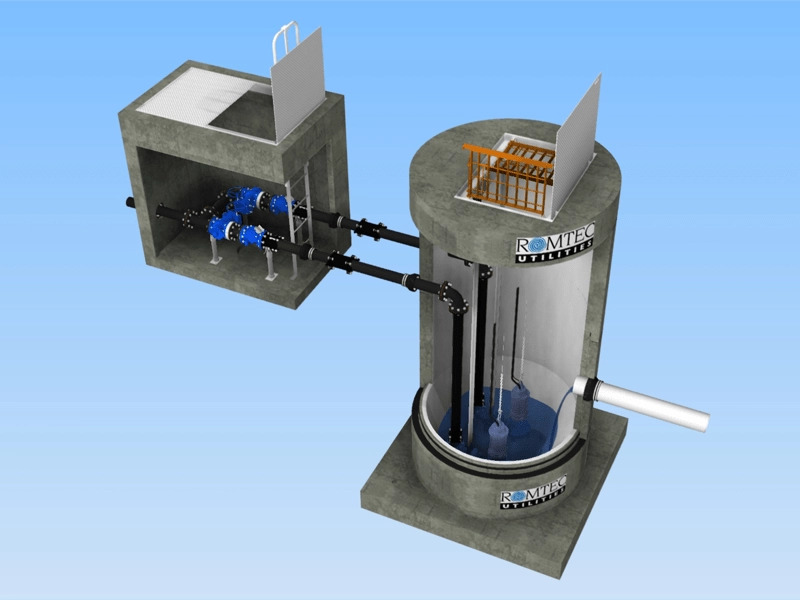
\includegraphics[width=0.75\textwidth]{alternative_1b.JPG}
    \caption{Three-dimensional rendering of a duplex submersible lift station showing wet well, pumps, and valve vault arrangement \cite{Romtec_StandardDuplex_LiftStation}.}
    \label{fig:alternative1_a}
\end{figure}

\subsection{Typical Application in Practice}
Duplex submersible pump stations are widely used by municipalities and developers for residential subdivisions across Mississippi. They provide centralized wastewater conveyance with redundancy, meeting state and local regulatory expectations for public ownership and maintenance under MDEQ’s \textit{Guidance for the Design of Publicly Owned Wastewater Facilities}~\cite{MDEQ_DesignGuidance_2025}.

\begin{figure}[H]
    \centering
    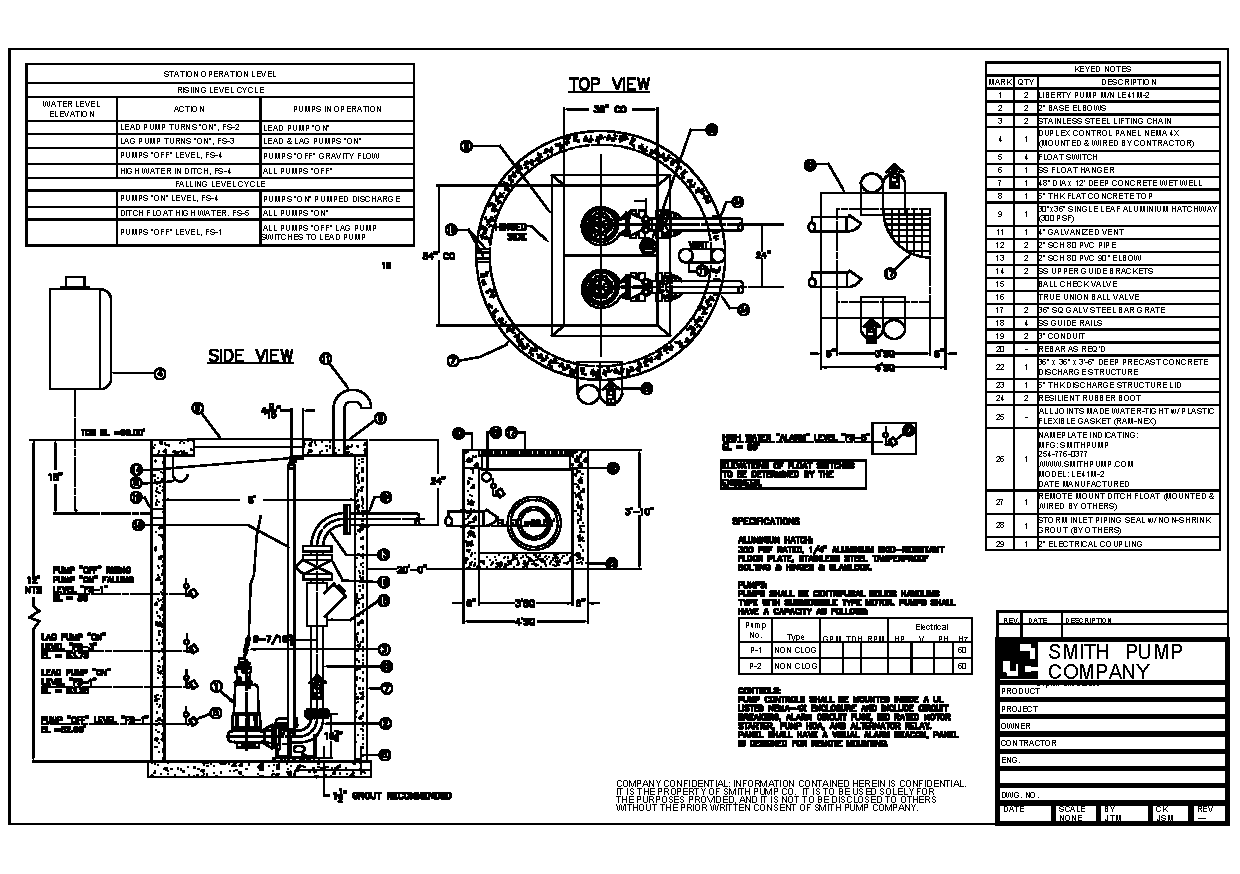
\includegraphics[width=1\textwidth]{alternative1b.pdf}
    \caption{Typical engineering drawing of a duplex submersible pump station with plan and section views, showing float controls, valves, and discharge piping layout \cite{SmithPump_DuplexSubmersible_LiftStation}.}
    \label{fig:alternative_1b}
\end{figure}

\subsection{Advantages}

The duplex submersible lift station offers high reliability through its redundant configuration. One pump remains on standby while the other operates under normal flow conditions, ensuring uninterrupted service during maintenance or in the event of a mechanical failure. This redundancy meets MDEQ’s requirements for small community wastewater systems and provides operational confidence for residential developments~\cite{MDEQ_DesignGuidance_2025}. The system also occupies a compact footprint, with most components installed below grade, minimizing land requirements and visual impact within the subdivision.

From an operational standpoint, municipal maintenance crews are highly familiar with this type of lift station, which simplifies inspection, troubleshooting, and part replacement. The station’s mechanical and electrical components are standard across many municipal systems, promoting ease of integration with existing maintenance programs. In terms of cost, this configuration provides a moderate initial investment compared to deep-gravity or distributed grinder systems while offering a lower life-cycle cost due to consolidated maintenance and shared control systems. The design is also expandable, as both the wet well and control panel can accommodate minor future flow increases without major reconstruction, making it a flexible and scalable solution for growing residential areas.

\subsection{Disadvantages}

The main disadvantage of the duplex submersible lift station lies in its mechanical and electrical dependence. Continuous power supply is required to sustain operation, meaning that outages can interrupt service unless backup power or emergency storage capacity is provided~\cite{NFPA_70_2023}. The system also faces potential odor and corrosion issues due to the accumulation of gases such as hydrogen sulfide within the wet well. Without adequate ventilation, coating, and chemical control, these gases can deteriorate structural and mechanical components over time~\cite{TenStates_RecommendedStandards_2014}.

Routine maintenance is another consideration, as the pumps, valves, and level sensors require regular inspection, lubrication, and periodic replacement. Although the duplex arrangement reduces the likelihood of total system downtime, the station still functions as a single point of failure for the subdivision. A complete station malfunction, while unlikely, would temporarily interrupt wastewater conveyance until repairs are completed. These limitations highlight the need for preventive maintenance, corrosion protection, and standby power provisions in the final design.

\subsection{Technical, Economic, Environmental, and Social Considerations}

From a technical perspective, the duplex submersible configuration provides consistent hydraulic performance by matching system flow and head requirements through controlled pumping operation. The system is capable of maintaining stable performance under both average and peak flow conditions while satisfying standard requirements for redundancy and wet-well capacity~\cite{MDEQ_DesignGuidance_2025,TenStates_RecommendedStandards_2014}. Economically, the lift station represents a balanced investment with moderate initial costs and predictable long-term maintenance expenses due to the use of centralized equipment and standardized components.

Environmentally, the system’s pressurized conveyance and sealed construction minimize the potential for exfiltration or infiltration, protecting both groundwater and surface water quality~\cite{EPA_LiftStation_DesignManual_2004}. The inclusion of proper ventilation and odor control also limits atmospheric emissions. Socially, the below-grade design reduces noise, odor, and visual impact, maintaining the residential character of the subdivision. Routine maintenance activities can be performed without major disruption to nearby residents, making this alternative both technically viable and socially acceptable for the Colebrooke Subdivision.


\section{Alternative 2 – Grinder Pump / Low-Pressure Sewer System}\label{sec:alt2}

\subsection{Description}
In this alternative, each residence, or in some cases a small cluster of homes, is equipped with an individual grinder-pump basin. The grinder pump collects wastewater from the house, grinds solids into a fine slurry, and discharges it through a small-diameter pressure service line into a shared low-pressure network that conveys flow to the downstream municipal sewer. The network typically consists of 1½- to 4-inch PVC or HDPE force mains operating under variable pressure. Check valves, isolation valves, and service connections are distributed throughout the subdivision rather than concentrated at a single central pump station~\cite{CFPUA_ResidentialGrinderPump_Diagram, LakesideMUD_LowPressureGrinderPump_SewerLayout}.

\begin{figure}[H]
    \centering
    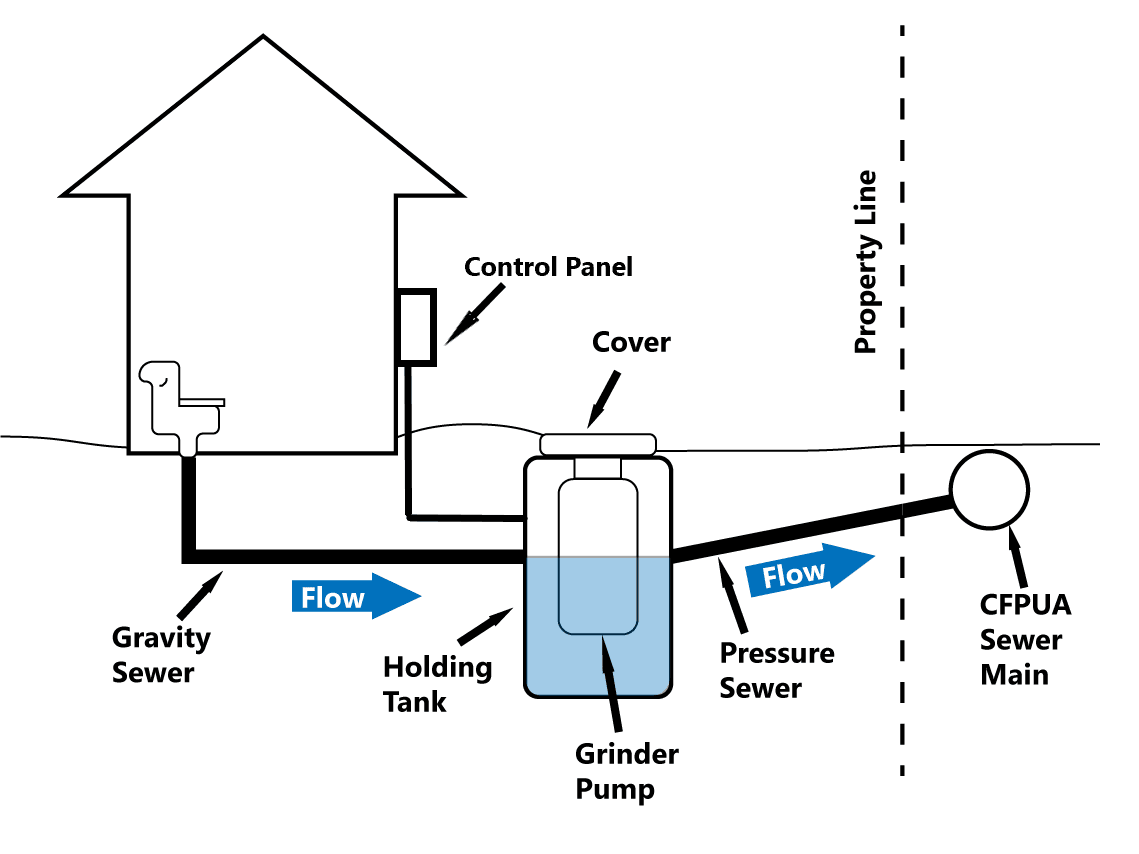
\includegraphics[width=0.8\textwidth]{alternative2a.png}
    \caption{Typical schematic of a household grinder-pump installation showing the holding tank, control panel, and connection to the low-pressure main~\cite{CFPUA_ResidentialGrinderPump_Diagram}.}
    \label{fig:alternative2a}
\end{figure}

\subsection{Typical Application in Practice}
Low-pressure grinder systems are commonly implemented in rural, hilly, or rocky areas where conventional gravity sewers would require deep excavation or multiple lift stations. They are also effective in regions with high groundwater tables or shallow rock, minimizing infiltration and exfiltration risks~\cite{EPA_LiftStation_DesignManual_2004}.

\begin{figure}[H]
    \centering
    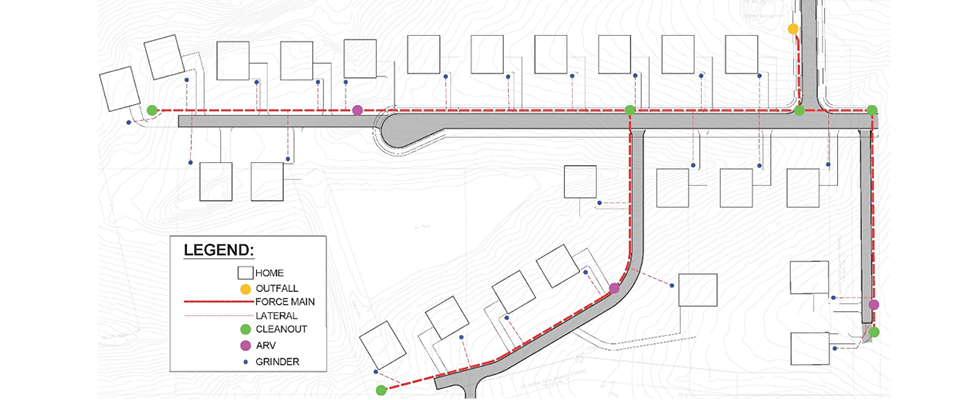
\includegraphics[width=1.05\textwidth]{alternative2b.png}
    \caption{Example layout of a low-pressure grinder-pump network in a residential subdivision, illustrating individual service laterals, shared force mains, and outfall connection~\cite{LakesideMUD_LowPressureGrinderPump_SewerLayout}.}
    \label{fig:alternative2b}
\end{figure}

\subsection{Advantages}

The grinder pump and low-pressure sewer system offers several advantages for small residential developments such as the Colebrooke Subdivision. The most notable benefit is the elimination of a central pump station, which removes the need for a large wet well, electrical control building, and associated mechanical infrastructure. This simplifies the overall system layout and reduces upfront construction costs. The system also allows for shallow installation, following natural surface grades with minimal trench depth. This characteristic reduces excavation costs, limits disturbance to existing soils, and minimizes potential conflicts with groundwater or unsuitable subgrade materials.

Another key advantage is the system’s flexibility in alignment. The small-diameter pressure mains can be routed around existing utilities, landscaping, or terrain constraints without major redesign, making it ideal for irregular or developed sites. The scalability of the system also supports incremental expansion; additional residences can be connected with minimal disruption or system modification. Furthermore, localized failures are limited in impact, as a malfunction typically affects only the individual home or a small group of houses served by that particular grinder pump, rather than the entire subdivision. This distributed configuration enhances overall system resilience and reduces the risk of widespread service interruption.

\subsection{Disadvantages}

Despite its flexibility, the grinder pump and low-pressure sewer system presents several drawbacks when applied to a small residential development. The most significant limitation is the requirement for multiple mechanical units, as each home must be equipped with its own grinder pump, float controls, and electrical connection. This greatly increases the total number of components to install, monitor, and maintain. Over time, this distributed setup can lead to higher cumulative maintenance costs compared to a centralized lift station.

Another major concern involves ownership and maintenance responsibility. It is often unclear whether individual homeowners, homeowners’ associations, or the municipality are responsible for servicing the pumps. This ambiguity can create management and liability challenges, especially in privately owned subdivisions. The system is also highly dependent on residential power supply, since each grinder unit relies on the homeowner’s electrical connection. During power outages, the basin provides only limited short-term storage capacity~\cite{NFPA_70_2023}.

Additional drawbacks include potential noise and odor issues if basins are not properly sealed or ventilated, particularly given their proximity to occupied dwellings. Furthermore, because each unit operates independently, the lifespan of pumps and controls may vary, resulting in non-uniform replacement cycles and complicating maintenance scheduling. Collectively, these disadvantages make long-term operation and management more complex than in a single centralized pumping system.

\subsection{Technical, Economic, Environmental, and Social Considerations}

From a technical standpoint, the grinder pump and low-pressure sewer system maintains adequate flow velocity within small-diameter pressure lines, effectively conveying wastewater with minimal sedimentation risk. However, the system’s performance depends heavily on the consistent operation of each individual pump. If one or more pumps fail, localized service interruptions or reduced conveyance efficiency may occur~\cite{EPA_LiftStation_DesignManual_2004}.

In economic terms, installation costs per home are often comparable to or slightly lower than those of a conventional gravity sewer, primarily due to the reduced excavation depth and smaller pipe diameters. However, the distributed nature of the system results in higher long-term operation and maintenance costs, as each home contains a separate pump, control system, and power source that must be individually serviced.

From an environmental perspective, the shallow and flexible installation minimizes excavation and overall land disturbance. Despite this advantage, the presence of multiple small pump basins increases the number of potential overflow points, especially during power outages or equipment failures.

In social terms, this configuration may be less preferred in planned residential developments where centralized municipal management of wastewater infrastructure is desired. The need for individual maintenance and the presence of mechanical equipment on private property can introduce management complexity and variability in system performance across users.

\section{Alternative 3 – Deep Gravity Sewer System}\label{sec:alt3}

\subsection{Description}
This alternative eliminates the need for a pump station by constructing a deep gravity sewer network that allows wastewater to flow naturally toward the downstream collection system. Achieving this configuration would require lowering the outlet elevation at the subdivision discharge point and installing deeper manholes and pipes along the main alignment. The design involves larger excavation depths, strict trench safety measures, and the use of suitable bedding materials to maintain pipe stability and prevent settlement. In areas with soft or saturated clay soils, shoring and dewatering would be necessary to ensure construction safety and long-term performance, as illustrated in Figure~\ref{fig:alternative3a}. 

\begin{figure}[H]
    \centering
    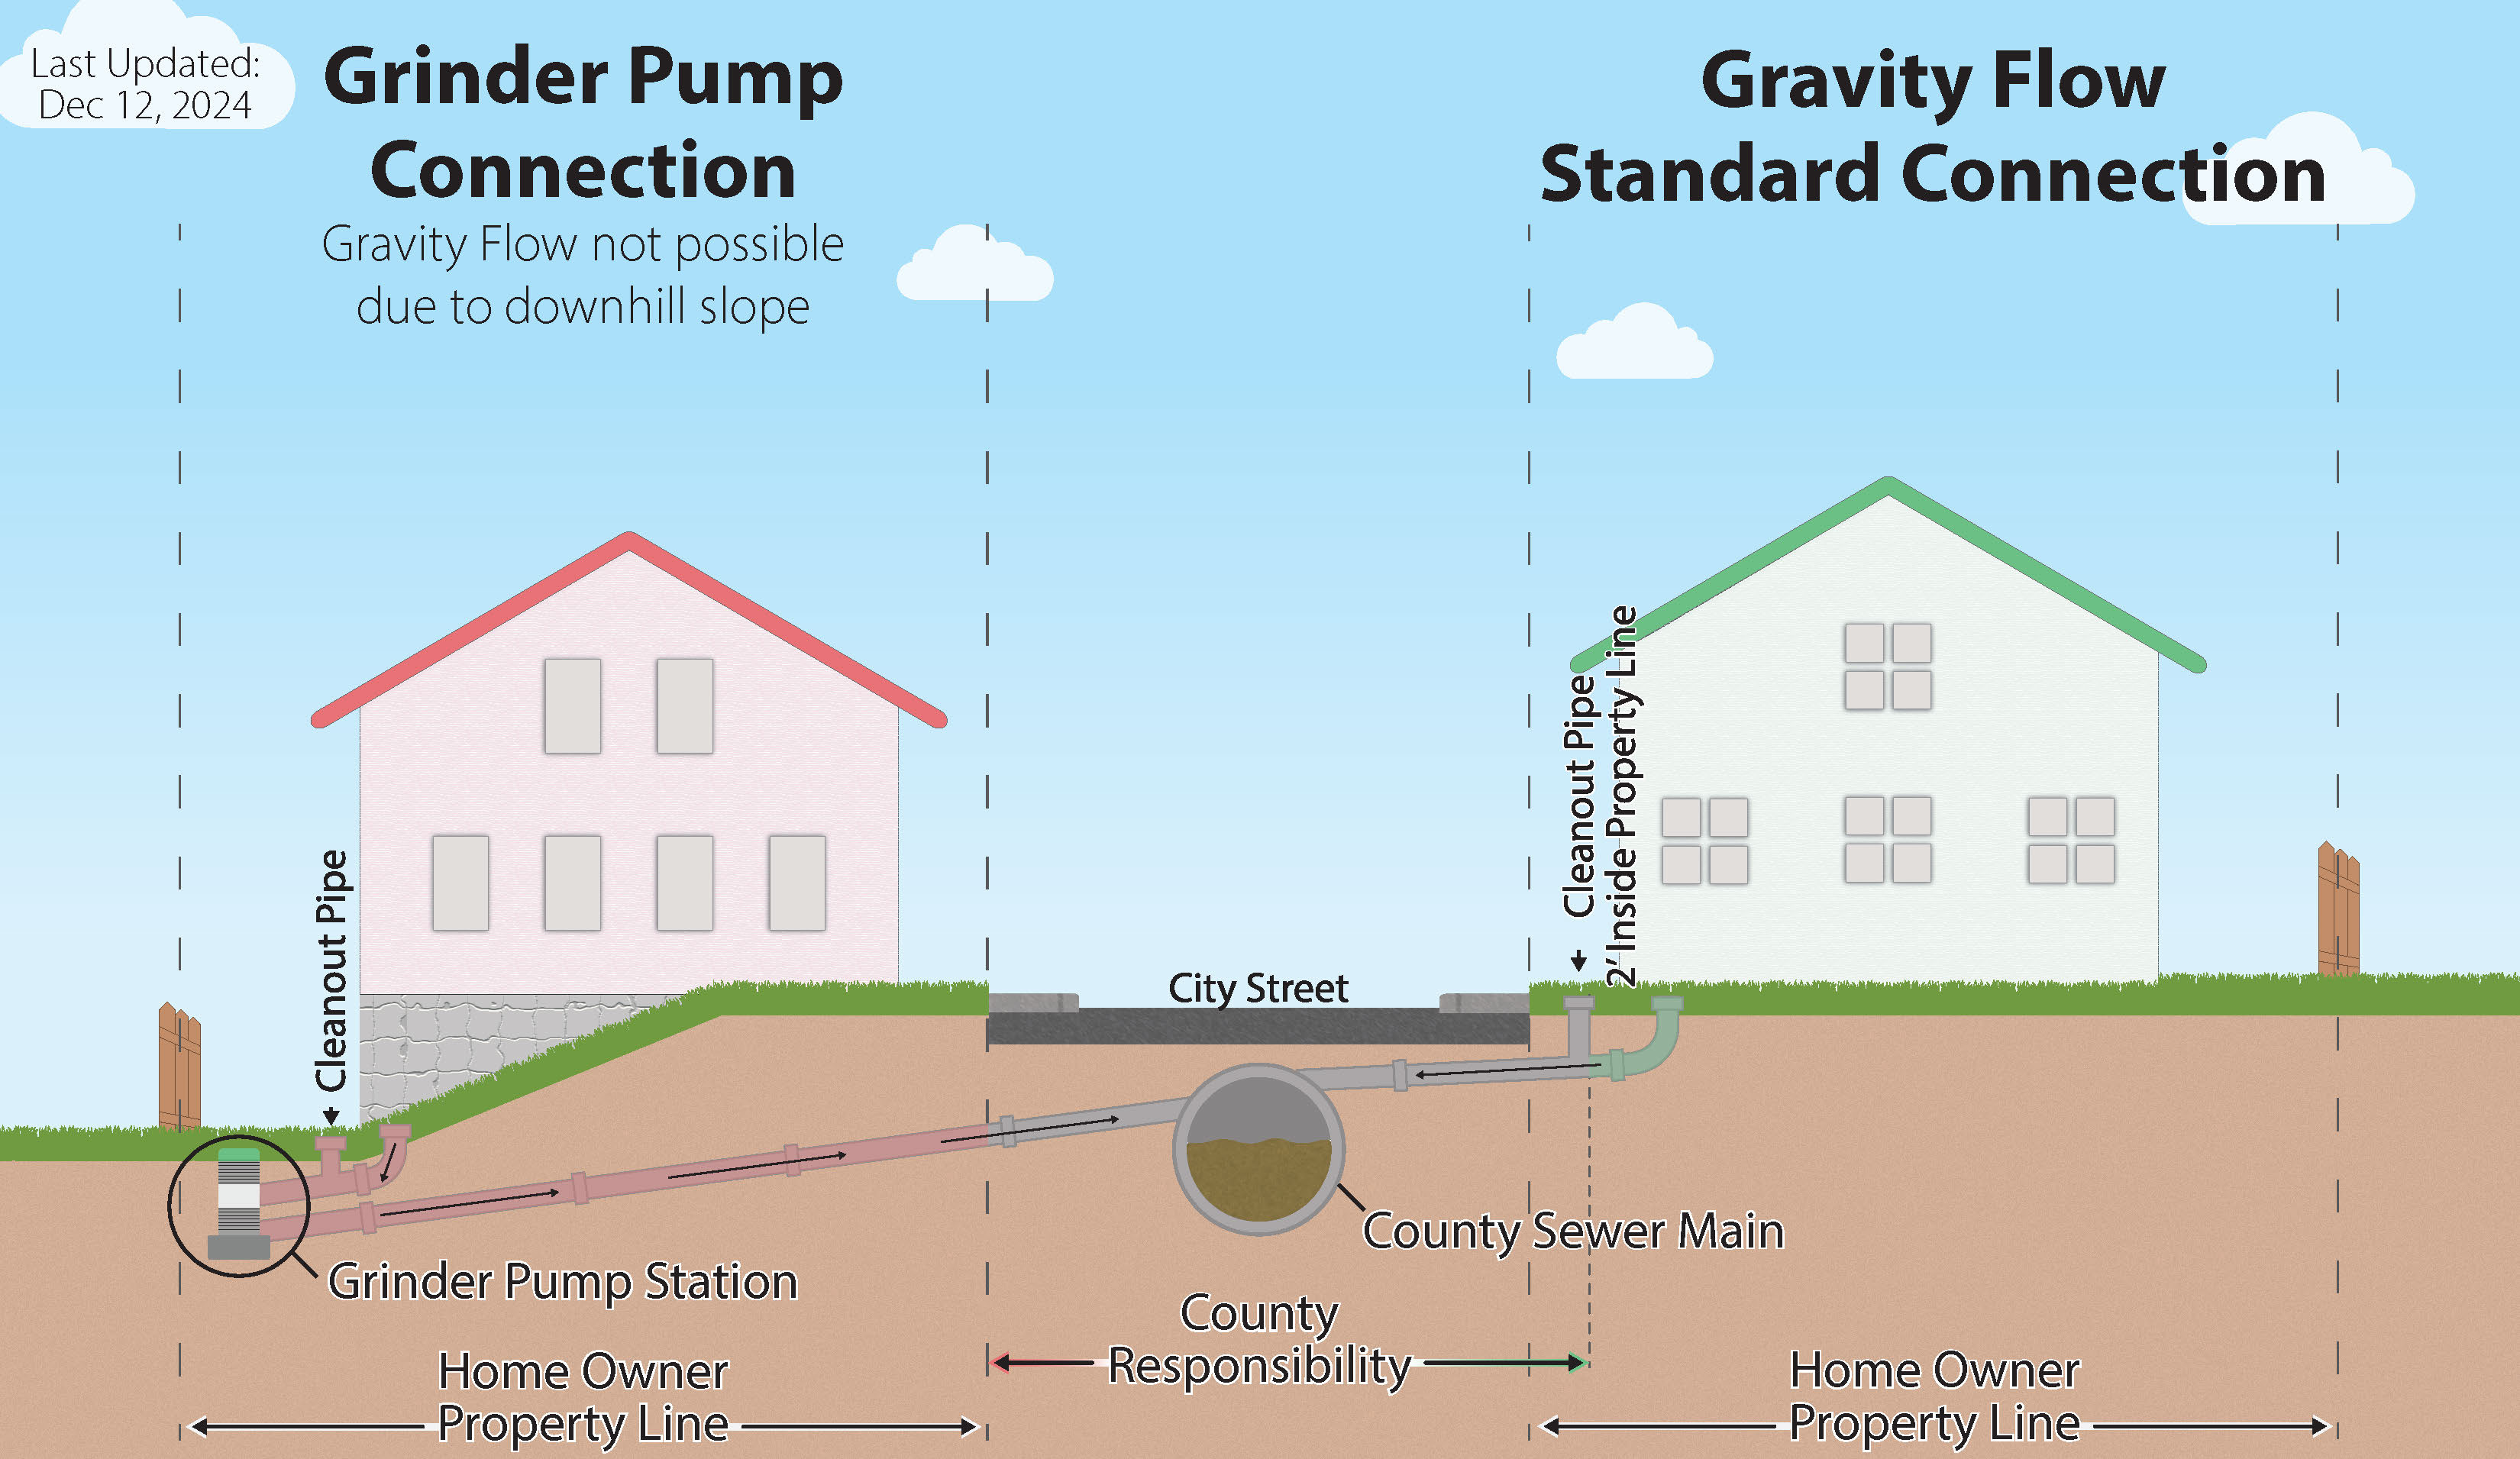
\includegraphics[width=0.9\textwidth]{alternative3a.jpg}
    \caption{Comparison of grinder-pump and gravity-flow connections showing how adequate elevation allows a standard gravity system while low terrain requires a pump installation~\cite{MauiRecovers_2024}.}
    \label{fig:alternative3a}
\end{figure}

\subsection{Typical Application in Practice}
Deep gravity systems are typically used when the ground elevation provides sufficient fall between the upstream service area and the outfall. These systems are ideal where excavation through stable soil layers is feasible and where long-term simplicity and low maintenance outweigh the higher initial construction cost.

\begin{figure}[H]
    \centering
    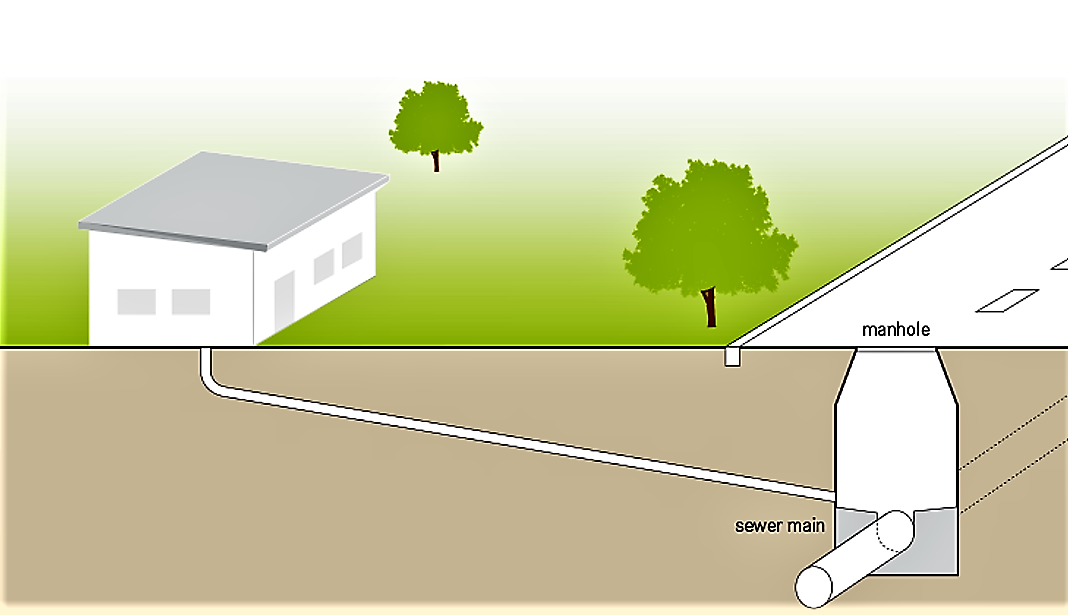
\includegraphics[width=0.85\textwidth]{alternative3b.png}
    \caption{Simplified cross-section of a deep gravity sewer showing pipe slope from a building connection to a manhole and main line under the roadway~\cite{Tilley_2014}.}
    \label{fig:alternative3b}
\end{figure}

\subsection{Advantages}
The primary advantage of the deep gravity sewer system lies in its simplicity and reliability. By relying entirely on gravitational flow, the system eliminates the need for pumps, electrical panels, or control mechanisms, significantly reducing operational complexity. Once constructed, the network operates passively and continuously, providing a dependable means of wastewater transport without requiring energy input. Because there are no moving parts, maintenance demands are limited to routine inspections and occasional cleaning of manholes, resulting in low life-cycle costs. The absence of mechanical equipment also ensures long-term reliability, as there are no mechanical failures that can disrupt service. Furthermore, the infrastructure remains fully underground, producing no visual or noise impact, which makes it highly acceptable to residential communities. From a sustainability perspective, this alternative promotes long-term energy conservation and minimizes the need for replacement parts or specialized operation.

\subsection{Disadvantages}
The main disadvantages of a deep gravity sewer system are associated with its high construction complexity and site limitations. Excavating to significant depths requires extensive labor, shoring, and dewatering, particularly in areas with weak or saturated soils where trench instability is a concern~\cite{Geotech_Colebrooke_2022}. These conditions not only increase construction time and cost but also introduce safety hazards that necessitate careful monitoring and support systems. Deep trenches may also conflict with existing or future utilities, such as water and gas lines, complicating coordination during both construction and maintenance. Repairs or new service connections at greater depths are considerably more difficult and expensive to perform, requiring specialized equipment and confined-space entry procedures. In some cases, topographic constraints may render this approach infeasible, particularly if the downstream sewer elevation is higher than the subdivision outlet~\cite{MDEQ_DesignGuidance_2025}. Overall, while deep gravity systems are operationally efficient once in place, their feasibility and cost-effectiveness are highly dependent on local soil conditions and elevation gradients.

\subsection{Technical, Economic, Environmental, and Social Considerations}
From a technical perspective, the deep gravity sewer offers a hydraulically simple and robust solution for wastewater conveyance. The flow relies solely on natural slope, making it inherently stable and resistant to operational interruptions. However, the design’s success depends heavily on precise surveying, soil strength, and groundwater conditions. Economically, deep gravity systems entail high initial capital investment due to excavation, shoring, and material costs, but their long-term operational and maintenance expenses are minimal compared to mechanical alternatives. Environmentally, the system operates without energy consumption and produces no emissions or noise once installed, posing minimal risk of spills or odors. The fully sealed pipeline and manhole network also reduce infiltration and exfiltration, preserving groundwater quality. From a social standpoint, this alternative is appealing because it eliminates above-ground equipment, visual clutter, and mechanical noise. Nonetheless, residents may experience temporary inconveniences during construction, such as road closures, vibrations, and hauling activities associated with deep trenching. In summary, while the deep gravity sewer represents the most sustainable and maintenance-free solution in the long term, it is only practical where favorable site topography and stable soil conditions exist.

\section{Final Selection}\label{sec:final_selection}

After a detailed evaluation of all three alternatives considering technical feasibility, constructability, cost, reliability, and long-term sustainability, the duplex submersible pump station with PVC force main was selected as the most appropriate option for the Colebrooke Subdivision wastewater conveyance system. This alternative best satisfies the design objectives established in the preliminary phase and meets both operational and regulatory requirements set forth by the Mississippi Department of Environmental Quality (MDEQ)~\cite{MDEQ_DesignGuidance_2025}.

The selected configuration demonstrates clear advantages in hydraulic performance and operational reliability. The existing topography of the subdivision does not provide sufficient elevation difference to sustain gravity flow throughout the service area, making a pumping solution essential. The duplex pump station ensures continuous operation by alternating between two pumps in a lead/lag cycle, maintaining stable discharge conditions and redundancy during maintenance or failure events. This arrangement aligns with common municipal practice for residential-scale lift stations and provides dependable performance under varying flow conditions~\cite{TenStates_RecommendedStandards_2014}.

From a constructability standpoint, the selected configuration allows installation at the natural low point of the subdivision with minimal excavation depth compared to deep gravity alternatives. The force main can be routed along the roadway corridor, allowing coordination with other infrastructure elements such as drainage and roadway construction. This integration simplifies construction sequencing and reduces overall site disturbance.

Maintenance and ownership considerations further support the selection of this centralized configuration. A single pump station allows for consolidated inspection, repair, and operational oversight by municipal staff. In contrast, a distributed grinder-pump network would require multiple individual service connections and private maintenance agreements, creating long-term management challenges. Centralized ownership under a municipal authority ensures consistent upkeep, protects public health, and maintains uniform service quality across all residences in the subdivision~\cite{EPA_LiftStation_DesignManual_2004}.

Economically, the centralized pump station provides a balanced solution over its service life. While the initial installation cost may be higher than some distributed alternatives, long-term operation and maintenance are simplified through centralized management and reduced system complexity. The use of standardized equipment and locally available components further supports cost-effective operation and maintenance~\cite{RSMeans_CostData_2025,ExcelFluidGroup_PumpComparison_2024}.

From an environmental and social perspective, the closed and pressurized nature of the force main minimizes the potential for infiltration, exfiltration, and odor generation. The below-grade installation reduces visual impacts and preserves the aesthetic character of the residential area. Collectively, these attributes contribute to sustainable infrastructure that supports public health, environmental protection, and community expectations for reliable wastewater management.

\section{Chapter Summary}\label{sec:chapter4_summary}

This chapter presented a comparative evaluation of three wastewater conveyance alternatives for the Colebrooke Subdivision: the duplex submersible pump station with PVC force main, the grinder pump and low-pressure sewer system, and the deep gravity sewer option. Each alternative was assessed in terms of hydraulic performance, constructability, cost, reliability, and environmental and social impacts. The analysis showed that the duplex submersible pump station provides the most balanced combination of technical feasibility, operational reliability, and economic efficiency. It satisfies the site’s hydraulic constraints, ensures centralized maintenance under municipal management, and offers long-term adaptability for future development. The findings of this analysis form the basis for the cost estimation and economic evaluation presented in the following chapter.


\newpage
\chapter{Final Design}

\section{Introduction to Final Design}

Following the evaluation of design alternatives and the establishment of governing design criteria, the wastewater conveyance system for the Colebrooke Subdivision is finalized as an integrated lift station and force main system. The selected configuration consists of a duplex submersible pump station that conveys wastewater through a pressurized force main to an existing municipal gravity sewer manhole located along Lewis Street. The system layout, including the pump station location, force main alignment, and downstream connection, is defined based on the subdivision survey and utility plan \cite{ProjectD_Colebrooke_2020}.

The force main extends $77.48~\text{ft}$ from the pump station to the receiving municipal manhole. Wastewater is collected from the subdivision gravity sewer network and delivered to the wet well, where it is pumped to the downstream system. The governing hydraulic input for the design is a peak wastewater inflow of $12.46~\text{gpm}$. The vertical difference between the wet well operating level ($299.00~\text{ft}$) and the receiving sewer invert ($309.28~\text{ft}$) produces a static head of $10.28~\text{ft}$, which forms the primary component of the system head requirements.

Based on the hydraulic analysis and system curve evaluation, the pump operating condition is established at $135.5~\text{gpm}$ and $12.08~\text{ft}$ of head. These parameters define the required performance of the pumping system and ensure that wastewater is reliably conveyed under expected operating conditions. This chapter presents the detailed hydraulic calculations, force main design, pump selection, and wet well sizing that form the basis of the final system design.



\newpage
% \section{Force Main Design and Hygraulic Analysis}
\subsection{Layout and System Configuration}

The geometric configuration of the wastewater conveyance system establishes the basis for the hydraulic analysis of the force main and pump station. The system consists of a submersible lift station located within the Colebrooke Subdivision that conveys wastewater through a pressurized force main to an existing municipal gravity sewer manhole.

The alignment of the force main, including stationing, pipeline length, and connection points, was defined using Autodesk Civil 3D based on the subdivision survey and utility layout. The pipeline extends from the pump station at Sta.~0+00.00 to the receiving municipal manhole at Sta.~0+77.48, resulting in a total force main length of $77.48~\text{ft}$. The plan layout, shown in Figure~\ref{fig:force_main_plan_ch5}, identifies the pump station location, force main alignment, and downstream connection to the municipal sewer system.

\begin{figure}[H]
\centering
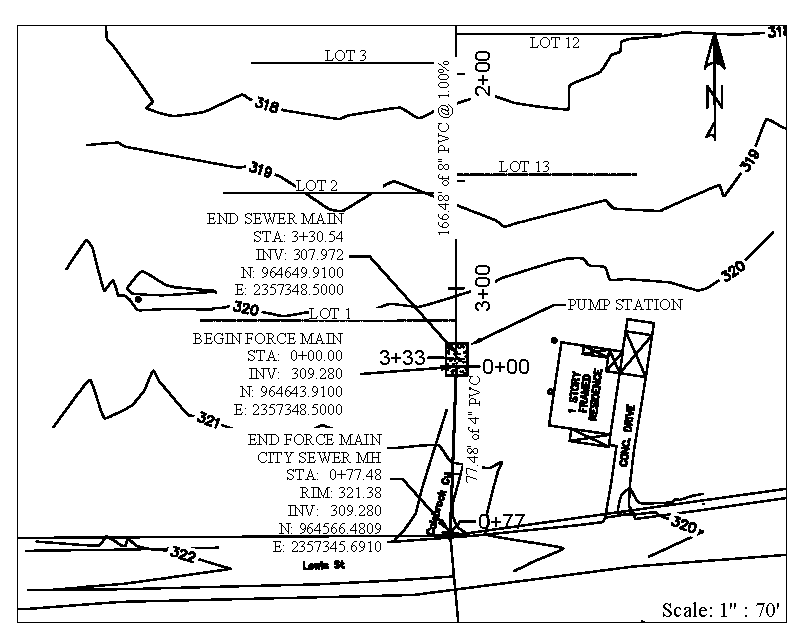
\includegraphics[width=\textwidth]{ForcemainLayoutPlan.pdf}
\caption{Final force main layout showing pump station location, pipeline alignment, and connection to the municipal sewer manhole.}
\label{fig:force_main_plan_ch5}
\end{figure}

The hydraulic profile of the system is defined by the wet well operating elevation of $299.00~\text{ft}$ and the discharge elevation of $309.28~\text{ft}$ at the receiving manhole. The profile, shown in Figure~\ref{fig:force_main_profile_ch5}, establishes the vertical relationship between the pump station and the municipal sewer system and defines the elevation difference governing the static head component of the hydraulic analysis.

\begin{figure}[H]
\centering
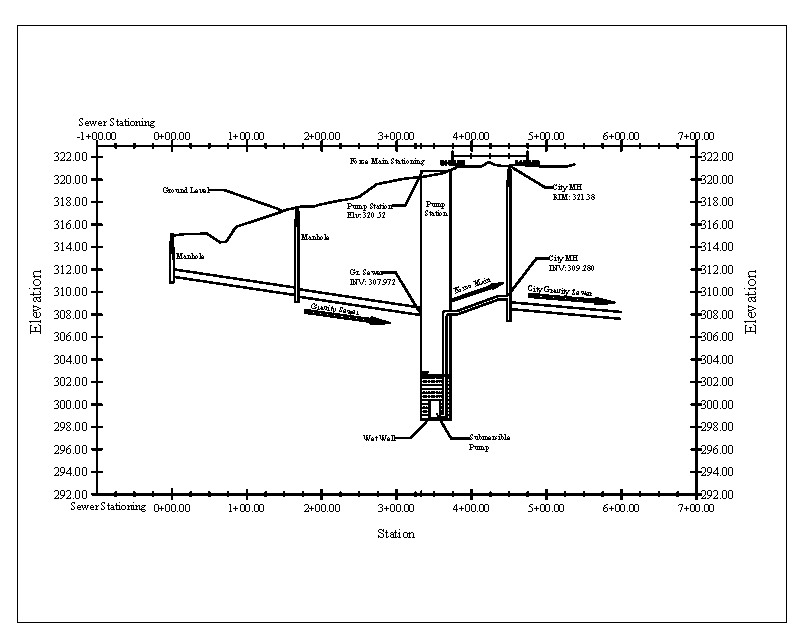
\includegraphics[width=\textwidth]{ForceMainLayoutProfile.pdf}
\caption{Hydraulic profile showing wet well elevation, force main alignment, and discharge elevation at the receiving municipal sewer manhole.}
\label{fig:force_main_profile_ch5}
\end{figure}

The plan and profile drawings provide the geometric inputs required for evaluating static head, friction losses, and minor losses in the force main. These parameters are used in the following sections to develop the total dynamic head and establish the system curve for pump selection.


\subsection{Design Parameters and Inputs}

The hydraulic design of the force main and pump station is based on the governing flow conditions, geometric configuration, and system parameters defined in Chapter~2. These inputs establish the basis for the evaluation of static head, friction losses, and minor losses used in the development of the total dynamic head.

The design flow for the system is taken as the peak wastewater inflow to the pump station, which is

\[
Q_{\text{peak}} = 12.46~\text{gpm}
\]

This flow represents the maximum anticipated inflow from the subdivision gravity sewer system and defines the minimum conveyance requirement for the pump station design.

In addition to the design flow, the hydraulic analysis requires geometric and system-specific parameters including the force main length, elevation data, pipe roughness coefficient, and minor loss coefficients. These parameters are summarized in Table~\ref{tab:design_inputs_ch5}.

\begin{table}[H]
\centering
\caption{Design Parameters for Hydraulic Analysis}
\label{tab:design_inputs_ch5}
\begin{tabular}{llll}
\toprule
\textbf{Parameter} & \textbf{Value} & \textbf{Unit} & \textbf{Description} \\
\midrule
Peak wastewater flow ($Q$) & 12.46 & gpm & Design inflow to pump station \\
Force main length ($L$) & 77.48 & ft & Distance from pump station to discharge \\
Discharge elevation ($z_d$) & 309.28 & ft & Receiving sewer manhole invert \\
Wet well elevation ($z_w$) & 299.00 & ft & Pump-off water surface elevation \\
Hazen--Williams coefficient ($C$) & 135 & -- & Pipe roughness coefficient \\
Minor loss coefficient ($K$) & 5.1 & -- & Combined fittings and valve losses \\
\bottomrule
\end{tabular}
\end{table}

These parameters define the physical and hydraulic characteristics of the system and are used in the subsequent sections to evaluate head losses and determine the total dynamic head required for pump selection.

% \newpage
% --------------------------------------------
% Chapter 3 — Force Main Design and Hydraulic Assessment
% --------------------------------------------

\section{Force Main Design and Hydraulic Assessment}


% -------------------------------------------------
% 3.0 Force Main Layout and System Configuration
% -------------------------------------------------
\subsection{Layout and System Configuration}

The physical configuration of the wastewater conveyance system was first established in order to determine the hydraulic parameters required for the pump station design. The system consists of a submersible lift station located within the Colebrooke Subdivision that conveys wastewater through a short force main to an existing city gravity sewer manhole. The geometric layout of the force main, including stationing, pipeline length, and connection points, was developed using Autodesk Civil 3D 2025.

The alignment of the pipeline was created using the \textit{Alignment} tools within Civil 3D, while the force main was modeled using the \textit{Pipe Network} tools to define pipe size, slope conditions, and the connection to the downstream manhole. This modeling process allowed accurate extraction of the pipeline length, elevations, and spatial relationships required for the hydraulic calculations performed in the following sections.

The resulting plan layout of the proposed force main and pump station is illustrated in Figure~\ref{fig:force_main_plan}. The drawing identifies the location of the pump station, the beginning and ending station of the force main, and the receiving city sewer manhole. The force main extends approximately $77.48~\text{ft}$ from the pump station to the receiving manhole where the wastewater discharges into the existing gravity sewer system. The drawing also provides key survey coordinates and elevation information used to establish the hydraulic profile of the system.

\begin{figure}[H]
\centering
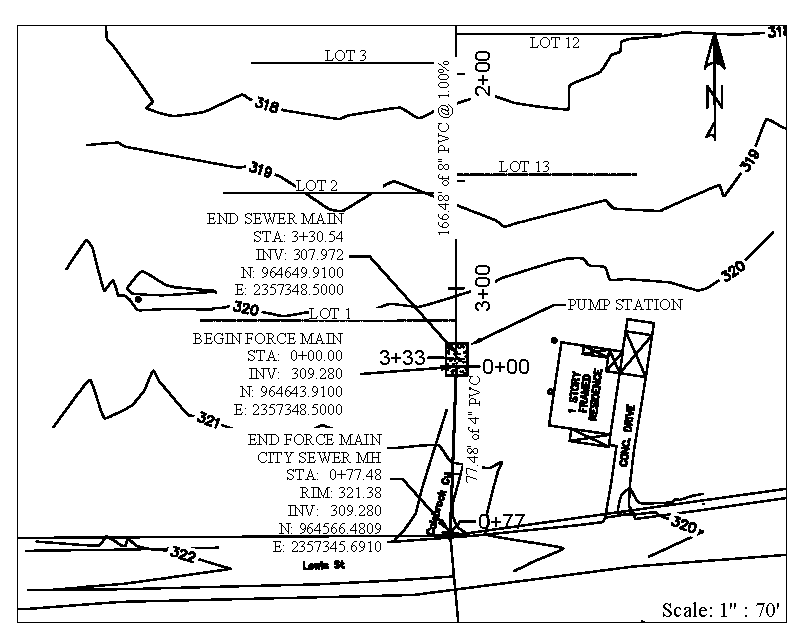
\includegraphics[
width=\textwidth,
]{ForcemainLayoutPlan.pdf}
\caption{Force main layout plan showing pump station location, pipeline alignment, and connection to the city sewer manhole.}
\label{fig:force_main_plan}
\end{figure}

The hydraulic relationship between the wet well and the receiving gravity sewer is illustrated in Figure~\ref{fig:pump_station_profile}. The profile diagram shows the wet well operating elevations, the discharge elevation at the receiving manhole, and the approximate length of the force main connecting the two structures. The wet well receives an inflow of $12.46~\text{gpm}$, and wastewater is conveyed through the force main to the downstream manhole located at an elevation of $309.28~\text{ft}$. These elevations define the vertical difference that produces the static head component used in the total dynamic head calculations.

\begin{figure}[H]
\centering
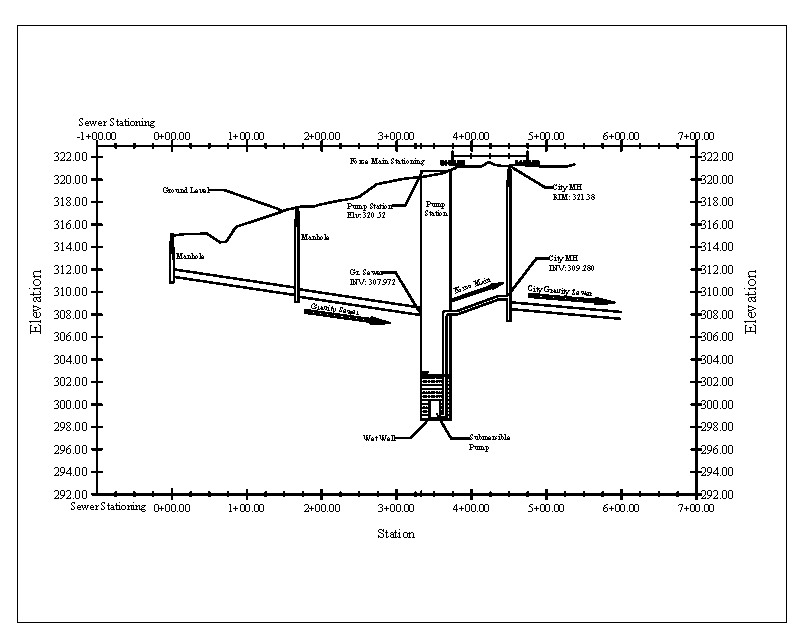
\includegraphics[
width=\textwidth,
trim={0.3in 0.6in 0.4in 0.6in},
clip
]{ForceMainLayoutProfile.pdf}
\caption{Hydraulic profile of the pump station showing wet well elevations, force main length, and discharge elevation at the receiving manhole.}
\label{fig:pump_station_profile}
\end{figure}

The plan and profile drawings provide the geometric basis for the hydraulic design of the system. The pipe length obtained from the Civil 3D alignment model, together with the discharge elevation and wet well water surface elevation, forms the basis for determining static head, friction losses, and minor losses in the force main. These parameters are used in the following sections to develop the system head requirements and establish the system curve for pump selection in accordance with the methodology described in the Jensen pump station design guidelines~\cite{ProjectD_Colebrooke_2020}.



% -------------------------------------------------
% 3.1 Force Main Material Selection
% -------------------------------------------------
\subsection{Force Main Material Selection}

The pressure pipeline connecting the proposed pump station to the downstream municipal sewer manhole functions as a force main that conveys wastewater under pressurized conditions. Selection of an appropriate pipe material is therefore an important design consideration because the material directly influences hydraulic performance, durability, constructability, and long-term operational reliability of the wastewater conveyance system.

For the Colebrooke Subdivision system, polyvinyl chloride (PVC) pressure pipe is selected as the force main material. PVC pipe is commonly used in wastewater conveyance applications due to its corrosion resistance, smooth internal surface, and relatively low installation cost compared with metallic pipe alternatives. The material is lightweight and relatively easy to install, which is advantageous for short pipeline segments such as the approximately 77.48~ft force main required for this project. These characteristics make PVC pipe a practical and reliable option for small lift station installations serving residential developments.

The selection of PVC pipe for the force main was made in consultation with applicable wastewater infrastructure guidance and pump station design references. Regulatory design guidance for publicly owned wastewater facilities recommends materials that provide corrosion resistance and long-term durability in sanitary sewer environments~\cite{MDEQ_DesignGuidance_2025}. In addition, pump station design practices described in the Jensen pump station design guidelines recognize PVC pressure pipe as a commonly used material for wastewater force mains due to its favorable hydraulic characteristics and ease of construction~\cite{Jensen_PumpStationDesignGuidelines_2012}.

A key hydraulic advantage of PVC pipe is its relatively smooth interior surface, which reduces friction losses during pressurized flow. In hydraulic analysis using the Hazen--Williams equation, this smoothness is represented by the Hazen--Williams roughness coefficient \(C\). For the PVC force main considered in this design, the following value is adopted:

\[
C = 135
\]

This value is consistent with commonly used design coefficients for new PVC pressure pipes and is suitable for evaluating friction losses in wastewater force mains using the Hazen--Williams formulation~\cite{Jensen_PumpStationDesignGuidelines_2012}. The selected roughness coefficient will be used in subsequent sections to estimate friction head losses within the force main during system operation.


% -------------------------------------------------
% 3.2 Force Main Diameter
% -------------------------------------------------
\subsection{Force Main Diameter}

An initial evaluation of the force main diameter was performed using the design flow provided by the sewer design team,
$Q = 12.46 \ \text{gpm}$.

The objective of this step is to evaluate the hydraulic performance of different pipe diameters and verify whether the resulting flow velocity satisfies typical wastewater force main velocity criteria.

The initial assumptions used for the preliminary hydraulic evaluation are summarized in Table~\ref{tab:diameter_inputs}.

\begin{table}[H]
\centering
\caption{Hydraulic Evaluation Parameters}
\label{tab:diameter_inputs}
\begin{tabular}{lll}
\toprule
\textbf{Parameter} & \textbf{Value} & \textbf{Unit} \\
\midrule
Design flow, $Q$ & 12.460 & gpm \\
Wet well water surface & 299.000 & ft \\
City sewer invert & 309.280 & ft \\
Static head, $H_s$ & 10.280 & ft \\
Force main length, $L$ & 77.480 & ft \\
Hazen--Williams coefficient, $C$ & 135 & -- \\
Total loss coefficient, $K$ (check + gate + bends + exit) & 5.100 & -- \\
Gravity, $g$ & 32.200 & ft/s$^2$ \\
Pump efficiency, $\eta$ & 0.60 & -- \\
\bottomrule
\end{tabular}
\end{table}

These parameters establish the baseline conditions used to evaluate candidate pipe diameters.

\subsubsection*{Hand Calculation Example (1-in Pipe)}

To demonstrate the procedure used in evaluating the force main diameter, a detailed hand calculation is presented for the case of a 1-inch diameter pipe.

\textbf{Convert Flow Rate}

The design flow must first be converted from gallons per minute to cubic feet per second.
\[
  \begin{aligned}
    & Q = 12.46 \ \text{gpm} \\
    &\Rightarrow Q = 12.46 \times \frac{1 \ \text{ft}^3}{7.48 \ \text{gal}} \times \frac{1}{60}\\
    &\therefore Q = 0.0278 \ \text{ft}^3/\text{s}
  \end{aligned}
\]


\textbf{Pipe Area}

For a 1-inch inside diameter pipe,
$D = 1 \ \text{in} = \frac{1}{12} \ \text{ft} = 0.0833 \ \text{ft}$

The pipe cross-sectional area is
\[
  \begin{aligned}
    & A = \frac{\pi D^2}{4} \\
    &\Rightarrow A = \frac{\pi (0.0833)^2}{4}\\
    &\therefore A = 0.0055 \ \text{ft}^2
  \end{aligned}
\]


\textbf{Velocity}

Velocity is calculated using the continuity equation:

\[
  \begin{aligned}
    & V = \frac{Q}{A} \\
    &\Rightarrow V = \frac{0.0278}{0.0055} \\
    &\therefore V = 5.09 \ \text{ft/s}
  \end{aligned}
\]

This velocity satisfies the typical minimum velocity requirement of $2~\text{ft/s}$.

\textbf{Friction Loss (Hazen--Williams)}

Friction loss in the force main is estimated using the Hazen--Williams equation:

\[
  \begin{aligned}
    & h_f = \frac{10.67\,L\,Q^{1.852}}{C^{1.852}D^{4.871}} \\
    &\Rightarrow h_f =
    \frac{10.67(77.48)(0.0278)^{1.852}}
    {(135)^{1.852}(0.0833)^{4.871}} \\
    &\therefore h_f = 4.24 \ \text{ft}
  \end{aligned}
\]

\textbf{Minor Losses}

Minor losses associated with fittings and valves are estimated using

\[
  \begin{aligned}
    & h_m = K\frac{V^2}{2g} \\
    &\Rightarrow h_m =
    5.10\left(\frac{5.09^2}{2\times32.2}\right) \\
    &\therefore h_m = 2.05 \ \text{ft}
  \end{aligned}
\]

\textbf{Total Dynamic Head}

\[
  \begin{aligned}
    & TDH = H_s + h_f + h_m \\
    &\Rightarrow TDH = 10.28 + 4.24 + 2.05 \\
    &\therefore TDH = 16.58 \ \text{ft}
  \end{aligned}
\]

\textbf{Brake Horsepower}

The required pump power is estimated using

\[
  \begin{aligned}
    & BHP = \frac{Q\times TDH}{3960\eta} \\
    &\Rightarrow BHP =
    \frac{12.46\times16.58}{3960\times0.60} \\
    &\therefore BHP = 0.087 \ \text{hp}
  \end{aligned}
\]

\subsubsection*{Diameter Comparison}

The above procedure was repeated for multiple pipe diameters.  
The resulting hydraulic performance values are summarized in Table~\ref{tab:diameter_comparison}.

\begin{table}[H]
\centering
\caption{Force Main Diameter Evaluation}
\label{tab:diameter_comparison}
\begin{tabular}{lccccc}
\toprule
 & \textbf{1 in} & \textbf{1.5 in} & \textbf{2 in} & \textbf{2.5 in} & \textbf{3 in} \\
\midrule
Area (ft$^2$) & 0.0055 & 0.0123 & 0.0218 & 0.0341 & 0.0491 \\
Velocity (ft/s) & 5.09 & 2.26 & 1.27 & 0.81 & 0.57 \\
Friction loss $h_f$ (ft) & 4.24 & 0.589 & 0.145 & 0.049 & 0.020 \\
Minor loss $h_m$ (ft) & 2.05 & 0.405 & 0.128 & 0.053 & 0.025 \\
TDH (ft) & 16.58 & 11.27 & 10.55 & 10.38 & 10.33 \\
BHP (hp) & 0.087 & 0.059 & 0.055 & 0.054 & 0.054 \\
Discharge pressure (psi) & 7.2 & 4.9 & 4.6 & 4.5 & 4.5 \\
Velocity check & OK & OK & $<2$ ft/s & $<2$ ft/s & $<2$ ft/s \\
\bottomrule
\end{tabular}
\end{table}

The results show that the velocity requirement of $2~\text{ft/s}$ is only satisfied for pipe diameters of $1~\text{in}$ and $1.5~\text{in}$ when using the calculated design flow. However, regulatory design guidance specifies that sewage force mains shall have a minimum diameter of $4~\text{in}$, except for grinder pump systems~\cite{MDEQ_DesignGuidance_2025}. Because the proposed system uses a conventional submersible sewage pump and is designed to convey solids up to approximately $3~\text{in}$ in diameter, smaller pipe diameters are not acceptable.

Accordingly, a $4$-inch PVC force main is selected as the design pipe diameter for the Colebrooke Subdivision pump station. The larger diameter provides adequate clearance for solids passage and complies with regulatory requirements for wastewater force mains.

The selected diameter will be used in the following sections to evaluate friction losses, minor losses, and the total dynamic head required for pump selection.


% -------------------------------------------------
% 3.3 Static Head Calculation
% -------------------------------------------------
\subsection{Static Head Calculation}

Static head represents the elevation component of the total energy that the pump must overcome to convey wastewater from the wet well to the downstream gravity sewer manhole. In wastewater lift station design, static losses arise from the difference in elevation between the discharge point and the water surface in the wet well. For a force main discharging to a gravity manhole, the static head is determined as the difference between the discharge elevation and the wet well water level~\cite{Jensen_PumpStationDesignGuidelines_2012}. 

To determine this value, the maximum elevation difference that the pump must overcome should be considered. This condition occurs when the water surface elevation in the wet well is at its lowest operating level, which is typically just above the pump shut-off elevation. Using the pump-off elevation therefore represents a conservative assumption for estimating the maximum static head. This elevation difference is a fundamental input in developing the system head requirements for the pump station and is consistent with the basis used in wastewater force main design guidance~\cite{MDEQ_DesignGuidance_2025}.

For the Colebrooke Subdivision pump station, the discharge elevation is taken as the invert elevation of the existing city sewer manhole, and the wet well reference elevation is taken as the pump-off water surface elevation. The relevant elevations are

\[
  \begin{aligned}
    & z_{\text{discharge}} = 309.28 \ \text{ft} \\
    & z_{\text{wet well}} = 299.00 \ \text{ft}
  \end{aligned}
\]

Accordingly, the static head is calculated as

\[
  \begin{aligned}
    & H_s = z_{\text{discharge}} - z_{\text{wet well}} \\
    &\Rightarrow H_s = 309.28 - 299.00 \\
    &\therefore H_s = 10.28 \ \text{ft}
  \end{aligned}
\]

Thus, the static head used for subsequent hydraulic calculations is

\[
  \begin{aligned}
    & H_s = 10.28 \ \text{ft}
  \end{aligned}
\]

The profile view of the pump station and discharge connection is shown in Figure~\ref{fig:force_main_profile}. This figure identifies the wet well water surface elevation of 299~ft, the discharge elevation of 309.28~ft at the receiving gravity sewer manhole, and the approximate force main length between the two points.

\begin{figure}[H]
    \centering
    % Adjust trim values as needed: trim = left bottom right top
    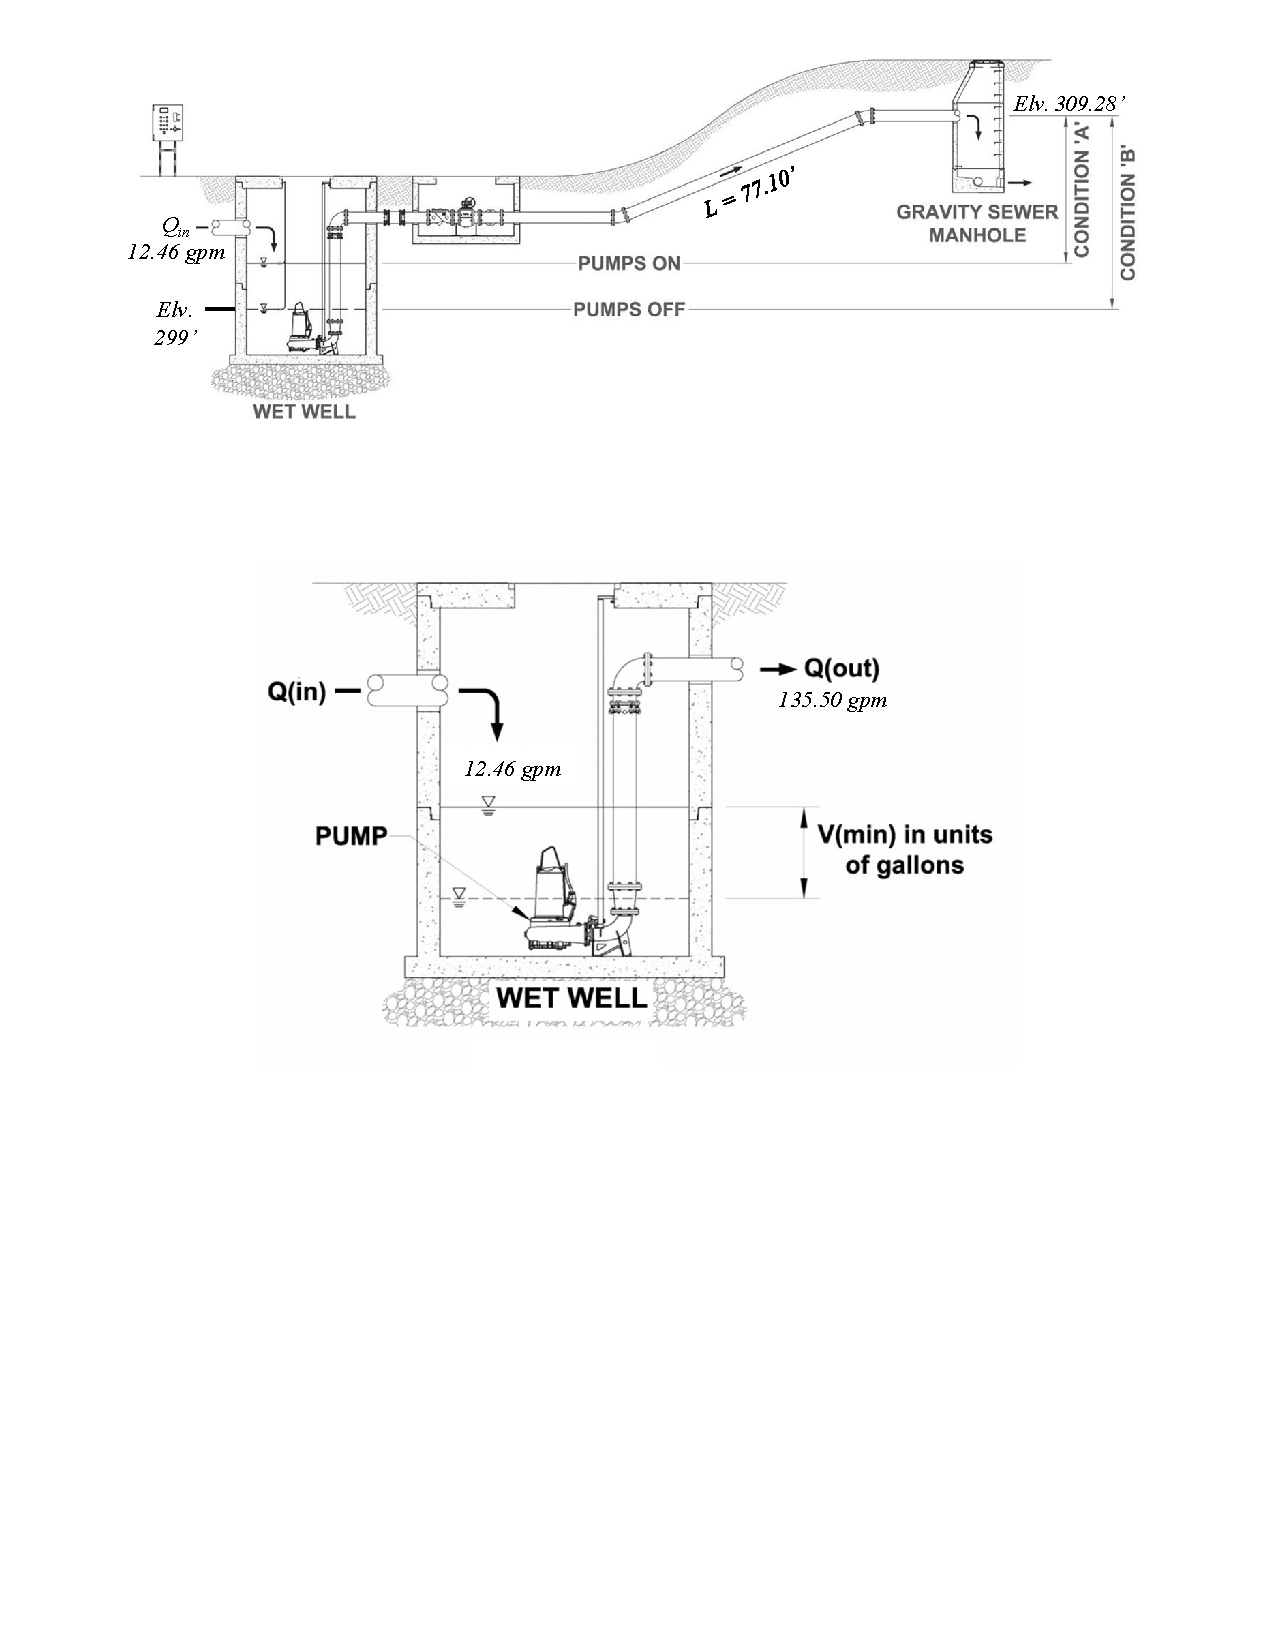
\includegraphics[
        page=1,
        width=\textwidth,
        trim={0.1in 8.0in 0.1in 0.1in},
        clip
    ]{forcemain_pump_figures.pdf}
    \caption{Pump station and force main profile showing wet well elevation, discharge elevation, and force main alignment.}
    \label{fig:force_main_profile}
\end{figure}

As illustrated in Figure~\ref{fig:force_main_profile}, the force main discharges to a gravity sewer manhole rather than to a pressurized system. Therefore, the static head is controlled only by the elevation difference between the receiving manhole invert and the wet well water surface. Jensen also notes that this value is not strictly fixed during operation because the wet well water surface fluctuates between the pumps-on and pumps-off elevations~\cite{Jensen_PumpStationDesignGuidelines_2012}. For conservative design and preliminary hydraulic analysis, the pumps-off elevation is used here, which produces the maximum static head condition.

The static head determined in this section forms the first component of the total dynamic head. The next step is to evaluate the friction losses that occur in the 4-in PVC force main during wastewater conveyance.

% -------------------------------------------------
% 3.4 Friction Loss in the Force Main
% -------------------------------------------------
\subsection{Friction Loss in the Force Main}

Dynamic losses in a pumping system arise primarily from friction as wastewater flows through the force main and associated fittings. Unlike static head, which is controlled by elevation difference, friction losses increase with flow rate and depend on the pipe material, pipe diameter, and internal flow conditions. Several methods exist to estimate friction losses in pressurized pipelines, including the Darcy--Weisbach equation and the Hazen--Williams equation. For wastewater lift station applications involving a simple force main discharging to gravity, the Hazen--Williams formulation is commonly adopted because it provides a relatively straightforward method for estimating friction losses while maintaining acceptable engineering accuracy~\cite{Jensen_PumpStationDesignGuidelines_2012}. In addition, many regulatory agencies allow or require the Hazen--Williams method for wastewater force main design~\cite{MDEQ_DesignGuidance_2025}.

The Hazen--Williams equation is applicable under turbulent flow conditions and is most reliable when velocities fall within a practical operating range. Jensen notes that velocities between approximately $3$ and $9~\text{ft/s}$ are desirable for wastewater force mains. Velocities below this range may allow solids to settle in the pipeline, while excessively high velocities can cause pipe abrasion or structural damage. These limits therefore provide a useful guideline when evaluating pump discharge conditions and developing the system curve for the force main~\cite{Jensen_PumpStationDesignGuidelines_2012}.

For this design, the friction-loss calculation will be based on a $4$-in PVC force main, a Hazen--Williams coefficient of $C = 135$, a force main length of $L = 77.48~\text{ft}$, and an initial inflow of $Q = 12.46~\text{gpm}$. These values are used because they correspond to the selected preliminary pipe material and diameter and the site layout established for the Colebrooke Subdivision system. A detailed sample calculation will be presented later with the system-curve development.

\pagebreak
The base form of the Hazen--Williams equation is written as

\begin{equation}
v = 1.318\, C\, R^{0.63} S^{0.54}
\end{equation}


where

$v$ = velocity ($\text{ft/s}$), 

$C$ = Hazen--Williams friction coefficient, 

$R$ = hydraulic radius ($\text{ft}$), 

$S$ = headloss slope ($\text{ft/ft}$)

For force main design, the conventional rearranged form used to estimate friction headloss is

\begin{equation}
h_f = 10.5\, L \left(\frac{Q}{C}\right)^{1.85} D^{-4.87}
\end{equation}

where

$h_f$ = friction headloss ($\text{ft}$)

$L$ = force main length ($\text{ft}$)

$Q$ = flow rate ($\text{gpm}$)

$C$ = Hazen--Williams friction coefficient ($-$)

$D$ = pipe diameter ($\text{in}$)

For PVC pipe, Jensen reports a wastewater design coefficient range of approximately $130$ to $145$, and the adopted value of $C = 135$ falls within this recommended range and also satisfies MDEQ guidelines.~\cite{Jensen_PumpStationDesignGuidelines_2012, MDEQ_DesignGuidance_2025}. Using the selected design parameters, the friction headloss for the $4$-in PVC force main at the initial inflow condition is very small relative to the static head because of the short pipe length and low flow rate. This friction component will be combined with static and minor losses in the following subsection to determine the total dynamic head of the system.


% -------------------------------------------------
% 3.5 Minor Loss Calculation
% -------------------------------------------------
\subsection{Minor Loss Calculation}

In addition to pipe-friction losses, the force main system also experiences localized energy losses as wastewater passes through fittings, valves, bends, and the discharge outlet. These localized losses are referred to as minor losses. Jensen notes that minor losses may be estimated either by the equivalent-length method or by using $K$-value coefficients assigned to individual fittings and appurtenances. For this project, the $K$-value method is adopted because it is straightforward and appropriate for a simple lift-station force main~\cite{Jensen_PumpStationDesignGuidelines_2012}.

Minor loss head is calculated using the following expression:

\begin{equation}
h_m = \sum K \frac{v^2}{2g}
\end{equation}



where

$h_m$ = minor headloss (ft)

$K$ = loss coefficient for each fitting or appurtenance ($-$)

$v$ = velocity of flow in the pipe (ft/s)

$g$ = gravitational acceleration ($32.2~\text{ft/s}^2$)

Based on the force main layout and coefficient values referenced from Jensen, the adopted minor-loss components include an entrance loss, one $90^\circ$ bend, one check valve, one valve, two $45^\circ$ bends, and the exit loss at the receiving manhole. The coefficients used in the hydraulic assessment are summarized in Table~\ref{tab:minor_losses}.

\begin{table}[H]
\centering
\caption{Minor Loss Coefficients Used in Hydraulic Assessment}
\label{tab:minor_losses}
\begin{tabular}{lccc}
\toprule
\textbf{Minor Loss Component} & \textbf{$K$} & \textbf{Number of Fittings} & \textbf{Sum $K$} \\
\midrule
Entrance & 0.25 & 1 & 0.25 \\
$90^\circ$ elbow & 0.25 & 1 & 0.25 \\
Check valve & 2.20 & 1 & 2.20 \\
Valve & 1.00 & 1 & 1.00 \\
$45^\circ$ bend & 0.18 & 2 & 0.36 \\
Exit & 1.00 & 1 & 1.00 \\
\midrule
 &  &  & $\Sigma K = 5.10$ \\
\bottomrule
\end{tabular}
\end{table}

Accordingly, the total minor-loss coefficient adopted for the system is

\[
\begin{aligned}
\sum K &= 5.10
\end{aligned}
\]

This value will be used together with the pipe velocity in the subsequent system-head calculations to determine the minor-loss component of the total dynamic head. A detailed sample computation of $h_m$ will be presented later with the system-curve development.


% -------------------------------------------------
% 3.6 Total Dynamic Head and System Curve
% -------------------------------------------------
\subsection{Total Dynamic Head and System Curve}

The total dynamic head (TDH) represents the total head that the pump must overcome to convey wastewater from the wet well to the downstream gravity sewer manhole. In a submersible lift station, TDH is the sum of the static head, the friction headloss in the force main, and the minor losses associated with bends, valves, and discharge conditions~\cite{Jensen_PumpStationDesignGuidelines_2012}. Jensen emphasizes that the system curve is the most important basis for pump selection because it defines the relationship between flow and the head required by the system. Rather than relying on approximate or assumed losses, TDH should be calculated at several flow rates so that the system curve can be developed and matched against candidate pump curves~\cite{Jensen_PumpStationDesignGuidelines_2012}.

The total dynamic head is expressed as

\[
\begin{aligned}
TDH &= \Delta H + h_f + h_m
\end{aligned}
\]

where

\begin{itemize}
\item $TDH$ = total dynamic head (ft)
\item $\Delta H$ = static head (ft)
\item $h_f$ = friction headloss (ft)
\item $h_m$ = minor headloss (ft)
\end{itemize}

Substituting the friction-loss and minor-loss expressions gives

\[
\begin{aligned}
TDH &= \Delta H 
+ (L)\,10.5\left(\frac{Q}{C}\right)^{1.85}D^{-4.87}
+ \Sigma K \frac{v^2}{2g}
\end{aligned}
\]

For the Colebrooke Subdivision pump station, the parameters used for the system-curve development are

\[
\begin{aligned}
\Delta H &= 10.28\ \text{ft} \\
D &= 4.00\ \text{in} \\
A &= 0.09\ \text{ft}^2 \\
C &= 135 \\
\Sigma K &= 5.10 \\
L &= 77.48\ \text{ft}
\end{aligned}
\]

Using these values, TDH was calculated for a range of discharge flow rates. The results are summarized in Table~\ref{tab:system_curve}.

\begin{table}[H]
\centering
\caption{System Curve Calculation for 4-in PVC Force Main}
\label{tab:system_curve}
\begin{tabular}{ccccccc}
\toprule
\textbf{Flow} & \textbf{Flow} & \textbf{Velocity} & \textbf{$h_m$} & \textbf{$h_f$} & \textbf{$\Delta H$} & \textbf{TDH} \\
(gpm) & (cfs) & (ft/s) & (ft) & (ft) & (ft) & (ft) \\
\midrule
0   & 0.00 & 0.0 & 0.00 & 0.0 & 10.28 & 10.3 \\
20  & 0.04 & 0.5 & 0.02 & 0.0 & 10.28 & 10.3 \\
40  & 0.09 & 1.0 & 0.08 & 0.1 & 10.28 & 10.5 \\
60  & 0.13 & 1.5 & 0.19 & 0.2 & 10.28 & 10.7 \\
80  & 0.18 & 2.0 & 0.33 & 0.4 & 10.28 & 11.0 \\
100 & 0.22 & 2.6 & 0.52 & 0.5 & 10.28 & 11.3 \\
120 & 0.27 & 3.1 & 0.74 & 0.8 & 10.28 & 11.8 \\
140 & 0.31 & 3.6 & 1.01 & 1.0 & 10.28 & 12.3 \\
160 & 0.36 & 4.1 & 1.32 & 1.3 & 10.28 & 12.9 \\
\bottomrule
\end{tabular}
\end{table}

\subsubsection*{Sample Calculation (Design Flow = 120 gpm)}

A sample calculation is shown below for a discharge flow of $120~\text{gpm}$, which is used as the design point for pump-curve evaluation.

For this system, the adopted design parameters are

\[
\begin{aligned}
\Delta H &= 10.28\ \text{ft} \\
D &= 4.00\ \text{in} = \frac{4}{12} = 0.333\ \text{ft} \\
A &= 0.09\ \text{ft}^2 \\
C &= 135 \\
\Sigma K &= 5.1 \\
L &= 77.48\ \text{ft} \\
g &= 32.2\ \text{ft/s}^2 \\
Q &= 120\ \text{gpm}
\end{aligned}
\]

\textbf{Convert flow from gpm to cfs}

\[
\begin{aligned}
Q &= 120\ \text{gpm}\times 
\frac{1\ \text{ft}^3}{7.48\ \text{gal}}\times 
\frac{1}{60\ \text{s/min}} \\
&\therefore Q = 0.267\ \text{ft}^3/\text{s}
\end{aligned}
\]

\textbf{Compute pipe velocity}

\[
\begin{aligned}
v &= \frac{Q}{A} \\
&\Rightarrow v = \frac{0.267}{0.0873} \\
&\therefore v = 3.06\ \text{ft/s}
\end{aligned}
\]

Using rounding consistent with the system-curve table,

\[
v \approx 3.1\ \text{ft/s}
\]

\textbf{Compute minor loss head}

\[
\begin{aligned}
&h_m = \Sigma K\frac{v^2}{2g} \\
&\Rightarrow h_m = 5.1\left(\frac{(3.06)^2}{2(32.2)}\right) \\
&= 5.1\left(\frac{9.36}{64.4}\right) \\
&= 5.1(0.1453) \\
&\therefore h_m = 0.741\ \text{ft}
\end{aligned}
\]

Thus,

\[
h_m \approx 0.74\ \text{ft}
\]

\textbf{Compute friction headloss}

Using the Hazen--Williams formulation adopted in this report,

\[
\begin{aligned}
&h_f = (L)10.5\left(\frac{Q}{C}\right)^{1.85}D^{-4.87} \\
&\Rightarrow h_f = (77.48)(10.5)
\left(\frac{120}{135}\right)^{1.85}(4)^{-4.87} \\
&\Rightarrow h_f = (77.48)(10.5)(0.804)(0.00117) \\
&\therefore h_f = 0.765\ \text{ft}
\end{aligned}
\]
Using rounding consistent with the system-curve table,

\[
h_f \approx 0.8\ \text{ft}
\]

\textbf{Compute total dynamic head}

\[
\begin{aligned}
TDH &= \Delta H + h_f + h_m \\
&\Rightarrow TDH = 10.28 + 0.77 + 0.74 \\
&\therefore TDH = 11.79\ \text{ft}
\end{aligned}
\]

Therefore,

\[
TDH \approx 11.8\ \text{ft}
\]

So, at a discharge flow of $120~\text{gpm}$, the system requires

\[
\boxed{TDH = 11.8\ \text{ft}}
\]

This point is used for pump-curve evaluation because it produces a force-main velocity of $3.1~\text{ft/s}$, which exceeds the MDEQ minimum velocity criterion of $2~\text{ft/s}$ and falls within the desirable wastewater transport range discussed in the Jensen guidance.

The resulting system curve is shown in Figure~\ref{fig:system_curve}

\begin{figure}[H]
\centering
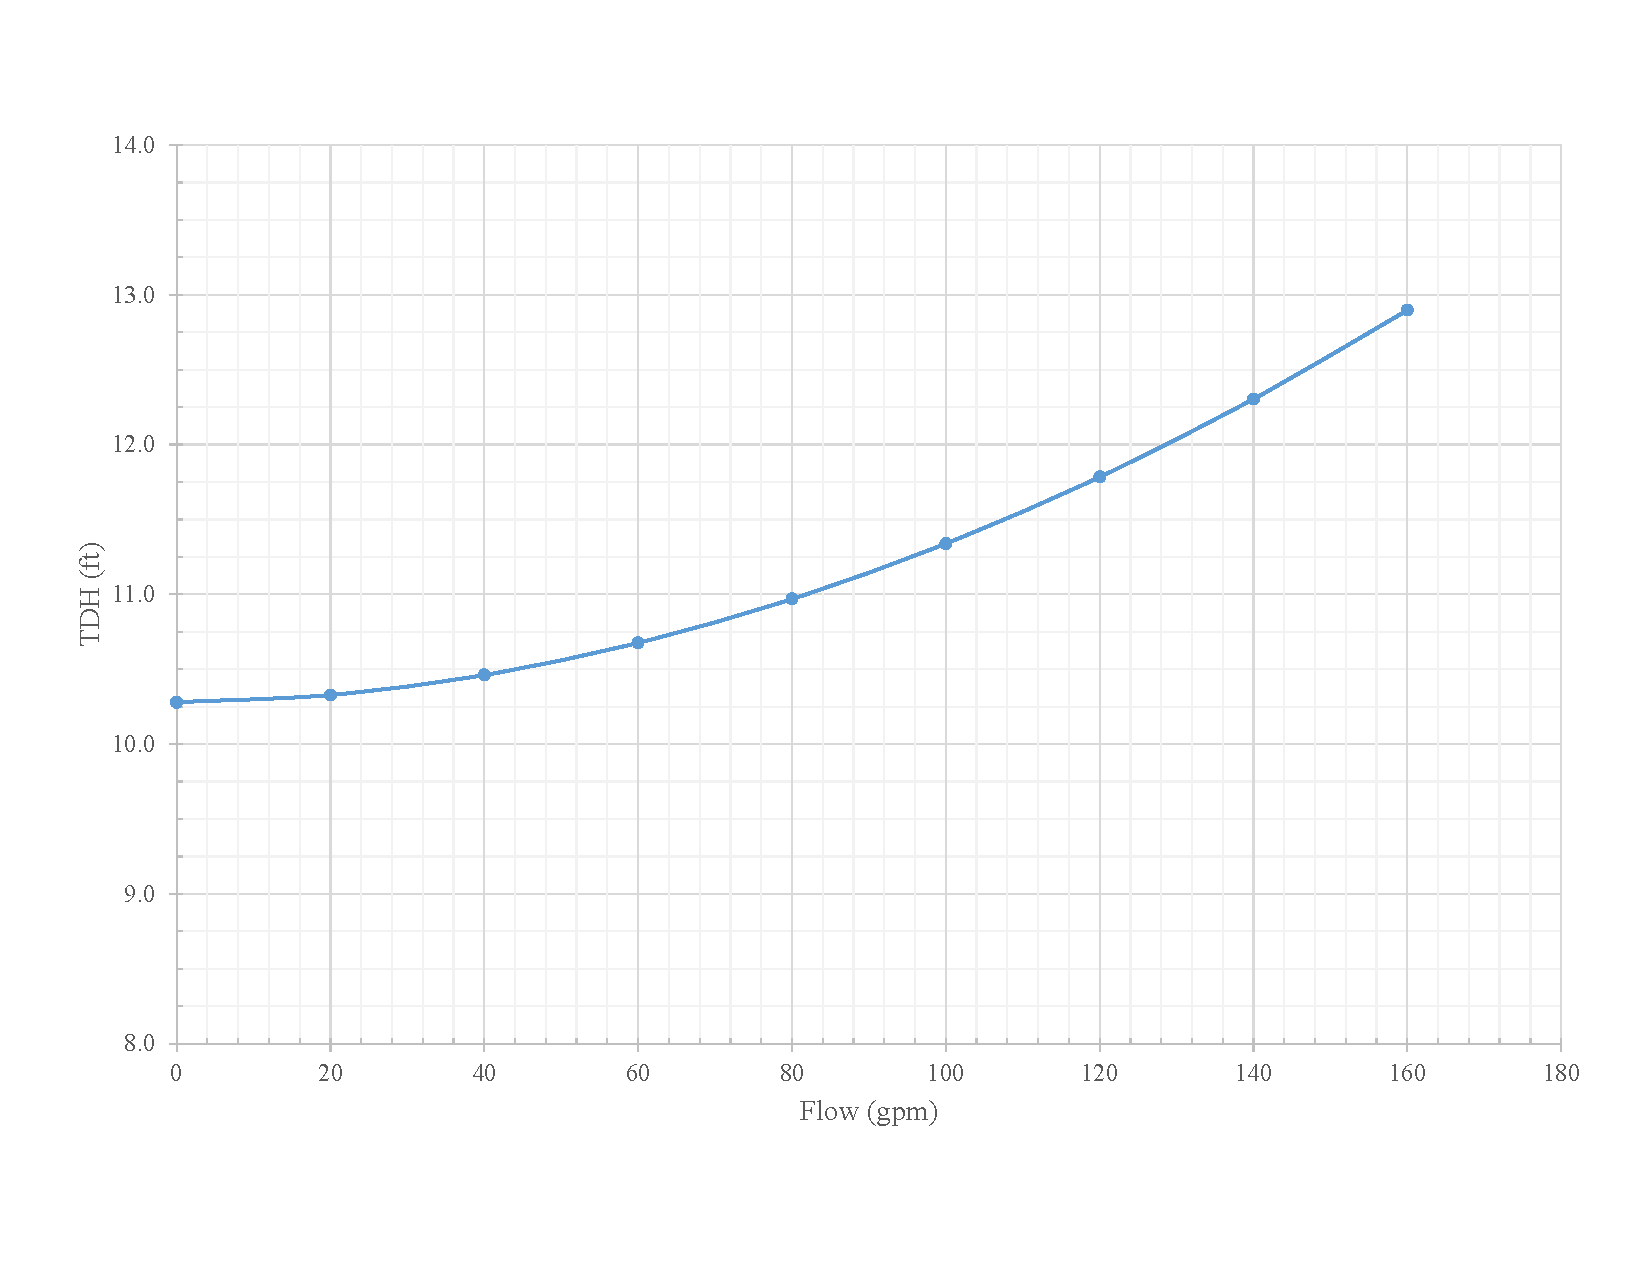
\includegraphics[
width=\textwidth,
% trim={0.2in 0.2in 0.2in 0.2in},
% clip
]{system-curve.pdf}
\caption{System curve showing total dynamic head versus flow for the 4-in PVC force main.}
\label{fig:system_curve}
\end{figure}

As shown in Figure~\ref{fig:system_curve}, the system head increases gradually with increasing flow because the static head remains constant while the friction and minor losses increase with discharge. This system curve will be used in the next section to evaluate candidate pump curves and identify an appropriate operating point for the Colebrooke Subdivision pump station.

\newpage
\section{Pump Selection}
% -------------------------------------------------
% 4.1 Pump Selection Criteria
% -------------------------------------------------
\subsection{Pump Selection Criteria}

Pump selection for the proposed lift station is based on the hydraulic requirements established from the system curve analysis developed in the previous chapter. The selected pump must be capable of delivering the required discharge flow while overcoming the calculated \textit{total dynamic head} ($TDH$) of the force main system. The operating point of the pump must therefore occur at the intersection of the pump performance curve and the system curve to ensure that the pump operates within an efficient and stable region of its performance range. This approach follows the pump station design methodology outlined in wastewater lift station design guidance~\cite{ProjectD_Colebrooke_2020}.

Because the station conveys raw municipal wastewater, the pump must be suitable for \textit{non-clog wastewater service} and capable of passing suspended solids commonly present in sanitary sewer systems. In this design, the pump is required to accommodate solids up to approximately $3~\text{in}$ in diameter in order to minimize the risk of clogging and ensure reliable operation under typical wastewater conditions. In addition to meeting the hydraulic head requirement, the pump must also operate efficiently at the selected design flow rate derived from the system curve.

Operational reliability is also an important consideration in wastewater lift station design. Therefore, the pump station is configured with a \textit{duplex pumping arrangement}, where one pump functions as the duty pump and the second pump provides redundancy and assists during higher inflow conditions. This configuration allows continuous operation of the station during maintenance or pump failure and is consistent with common wastewater lift station design practices~\cite{ProjectD_Colebrooke_2020}.


% -------------------------------------------------
% 4.2 Pump Curve Matching
% -------------------------------------------------
\subsection{Pump Curve Matching}

Pump selection is performed by comparing the system curve developed in the previous chapter with the manufacturer's pump performance curves. The system curve represents the relationship between flow rate and the total dynamic head required by the piping system. As flow increases, friction and minor losses increase, resulting in a corresponding increase in the total dynamic head that the pump must overcome. The system curve therefore defines the hydraulic resistance of the force main system.

Pump manufacturers provide pump performance curves that illustrate the relationship between flow rate and head produced by a specific pump model. By plotting the system curve together with the pump performance curve, the operating point of the pump can be identified. The operating point occurs at the intersection of the two curves and represents the flow and head conditions at which the pump will operate within the system.~\cite{Jensen_PumpStationDesignGuidelines_2012}

The pump selected for the proposed lift station must therefore have a performance curve that intersects the system curve near the desired design flow while maintaining acceptable efficiency and stable operation. This procedure ensures that the selected pump can deliver the required flow against the calculated system head while operating within the recommended performance range for wastewater pumping systems~\cite{ProjectD_Colebrooke_2020}.



% -------------------------------------------------
% 4.3 Selected Pump Operating Point
% -------------------------------------------------
\subsection{Selected Pump Operating Point}

The final pump duty point was determined by comparing the system curve developed in Chapter 3 with manufacturer pump performance curves using the Sulzer ABSEL pump selection tool. ABSEL is a web-based hydraulic selection platform developed by Sulzer that allows users to configure application conditions, input the required duty point, and evaluate pump performance curves for water and wastewater applications. The tool enables users to select pumps by defining the operating flow and head requirements and provides outputs including pump curves, hydraulic efficiency, dimensional drawings, and product data sheets. This procedure follows standard pump selection practice in wastewater lift station design where the system curve is compared with manufacturer pump curves to determine the operating point of the pump \cite{Jensen_PumpStationDesignGuidelines_2012,EPA_LiftStation_DesignManual_2004}. The ABSEL tool used for pump selection is provided by Sulzer for water and wastewater pump sizing and hydraulic performance evaluation \cite{Sulzer_ABSEL}.

The design operating point was selected from the system curve developed earlier. At a flow of $120~\text{gpm}$, the calculated system head is $11.8~\text{ft}$. This operating condition satisfies the minimum velocity requirement for wastewater transport within the force main and lies within the hydraulic operating range of the system. The duty point was entered into the Sulzer ABSEL selection tool to identify a pump whose performance curve intersects the system curve near this operating condition. The resulting pump selection corresponds to a Sulzer submersible wastewater pump, model XFP100C VX 1$\sim$ (wet pit installation) equipped with a vortex impeller designed for handling sewage containing suspended solids and fibrous material \cite{Sulzer_PumpCatalog_2024}.


\begin{figure}[H]
\centering
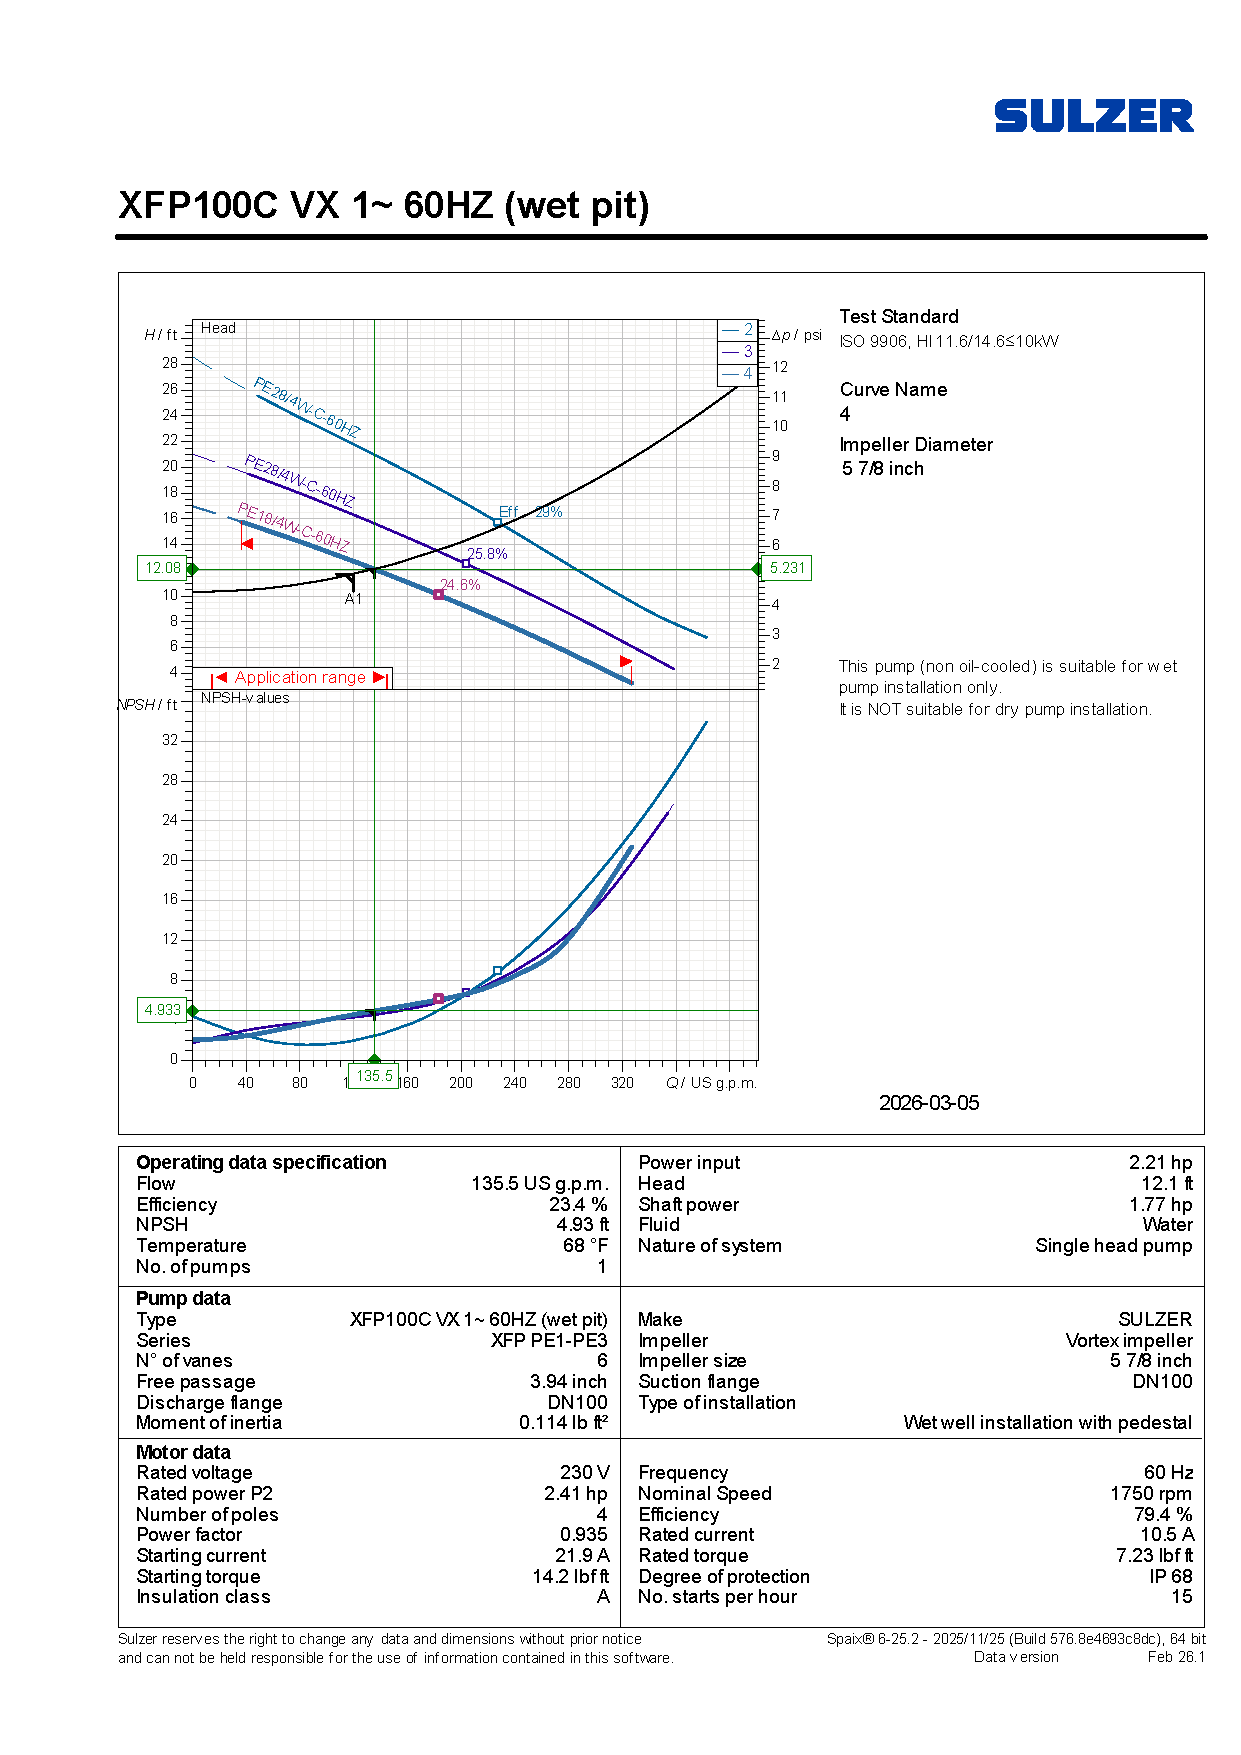
\includegraphics[
width=\textwidth,
trim={0.79in 4.3in 2.7in 2in},
clip
]{sulzer_xfp100c_curve.pdf}
\caption{Pump performance curve showing intersection with the system curve and selected operating point for the Sulzer XFP100C VX pump.}
\label{fig:pump_curve_intersection}
\end{figure}

The intersection between the system curve and the manufacturer pump performance curve defines the operating point of the selected pump. As illustrated in Figure~\ref{fig:pump_curve_intersection}, the selected Sulzer pump produces $135.5~\text{gpm}$ at a head of $12.08~\text{ft}$, which aligns with the hydraulic requirements of the system. This intersection confirms that the selected pump can deliver the required discharge while overcoming the calculated system head losses. The motor model at this point is PE 18/4W.

The performance data corresponding to the selected operating point are summarized in Table~\ref{tab:pump_operating_point}.

\begin{table}[H]
\centering
\caption{Selected Pump Operating Conditions}
\label{tab:pump_operating_point}
\begin{tabular}{lc}
\toprule
\textbf{Parameter} & \textbf{Value} \\
\midrule
Flow & 120 gpm (system design point) \\
Pump operating flow & 135.5 gpm \\
Total Dynamic Head & 12.08 ft \\
Hydraulic efficiency & 23.38 \% \\
Shaft power & 1.765 hp \\
\bottomrule
\end{tabular}
\end{table}

According to the manufacturer performance data, the selected pump operates at $135.5~\text{gpm}$ and $12.08~\text{ft}$ of head, with a hydraulic efficiency of $23.38~\%$ and a shaft power requirement of $1.765~\text{hp}$. The pump utilizes a vortex impeller that allows the passage of wastewater containing suspended solids and fibrous materials, which is a typical requirement for municipal wastewater pumping systems \cite{MetcalfEddy_Wastewater_2014}. The unit is designed for wet well installation and is equipped with an IE3 premium-efficiency motor operating at $1772~\text{rpm}$ \cite{Sulzer_PumpCatalog_2024}.

These performance parameters confirm that the selected Sulzer pump satisfies the hydraulic requirements of the lift station and provides adequate solids-handling capability for wastewater service. The motor power requirement identified from the manufacturer performance data will be used in the following section to determine the electrical and power requirements of the pump station.


% -------------------------------------------------
% 4.4 Pump Power Requirement and Motor Configuration
% -------------------------------------------------
\subsection{Pump Power Requirement and Motor Configuration}

The power requirement for the selected pump was obtained directly from the manufacturer performance data provided through the Sulzer ABSEL pump selection tool. At the selected operating condition, the Sulzer XFP100C VX 1$\sim$ (wet pit) pump delivers $135.5~\text{gpm}$ at $12.08~\text{ft}$ of head with a shaft power requirement of $1.765~\text{hp}$ and a motor output of $2.414~\text{hp}$. These values are taken from the manufacturer pump performance curves and therefore represent the required power for the selected operating point of the system \cite{Sulzer_ABSEL,Sulzer_PumpCatalog_2024}. The pump is equipped with a Sulzer PE18/4W motor operating at $230~\text{V}$, $60~\text{Hz}$, and $1772~\text{rpm}$, which defines the electrical capacity required for the lift station pump.

The selected unit utilizes a vortex impeller, which is commonly used in wastewater pumping applications. Jensen explains that vortex impellers are positioned toward the rear of the pump casing so that the rotating impeller generates a forced vortex that transports solids through the pump without requiring them to pass directly through the impeller vanes. This configuration improves reliability in sewage applications by allowing the passage of fibrous material and suspended solids while reducing the likelihood of clogging \cite{Jensen_PumpStationDesignGuidelines_2012}. For the Colebrooke Subdivision lift station, the vortex impeller was selected because reliability and solids-handling capability are critical for residential wastewater service.

The internal configuration of a typical submersible wastewater pump is illustrated in Figure~\ref{fig:submersible_pump_components}. The diagram shows the major mechanical elements including the motor assembly, shaft, bearings, mechanical seals, oil chamber, and impeller. These components work together to transmit motor power to the impeller while protecting the motor and bearings from wastewater intrusion.

\begin{figure}[H]
\centering
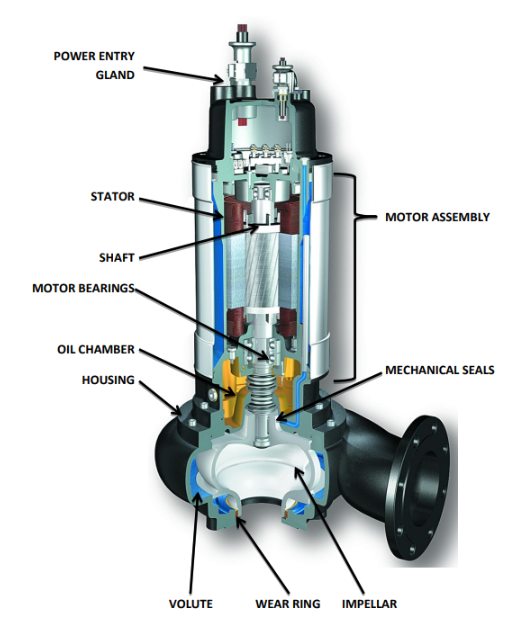
\includegraphics[width=0.7\textwidth]{components_of_a_pump.png}
\caption{Internal components of a submersible wastewater pump. Courtesy: Homa Pumps. \cite{HOMA_HazenWilliams_1998}}
\label{fig:submersible_pump_components}
\end{figure}

The selected pump incorporates a sealed submersible motor with an oil chamber and dual mechanical seals, which protect the motor and bearings from liquid intrusion during operation. Oil-filled submersible motors are commonly used in wastewater pumps because the oil improves heat transfer and provides continuous lubrication for internal components. The pump assembly also includes radial and axial load-supporting bearings designed by the manufacturer to withstand the hydraulic loads generated during pumping operation \cite{Jensen_PumpStationDesignGuidelines_2012}. These features ensure reliable operation of the pump under continuous wastewater service conditions.

\newpage
% =================================================
% Chapter 5 — Wet Well Recommendations
% =================================================

\section{Wet Well Recommendations}

% -------------------------------------------------
\subsection{Introduction to Wet Well Design}
% -------------------------------------------------

Once the system curve has been established and the selected pump has been matched to that system, the next step is to size the wet well and define the operating control elevations. For the Colebrooke Subdivision lift station, the selected pump is the Sulzer XFP100C VX 1$\sim$ (wet pit) with vortex impeller. The selected operating point from the pump selection process is $135.5~\text{gpm}$ at $12.08~\text{ft}$ of head, and the system inflow to the wet well at peak conditions is $12.46~\text{gpm}$. These values were used to size the minimum storage volume and define the control elevations for the duplex wet well. The project itself includes pump station design and force main design as one of the major infrastructure components of the subdivision \cite{ProjectD_Colebrooke_2020}, and the working inflow and pump discharge values used in the wet well sketches are shown in the reference figures prepared for this design.

The conceptual arrangement of the wet well and pump configuration is illustrated in Figure~\ref{fig:wetwell_storage_config}.

\begin{figure}[H]
\centering
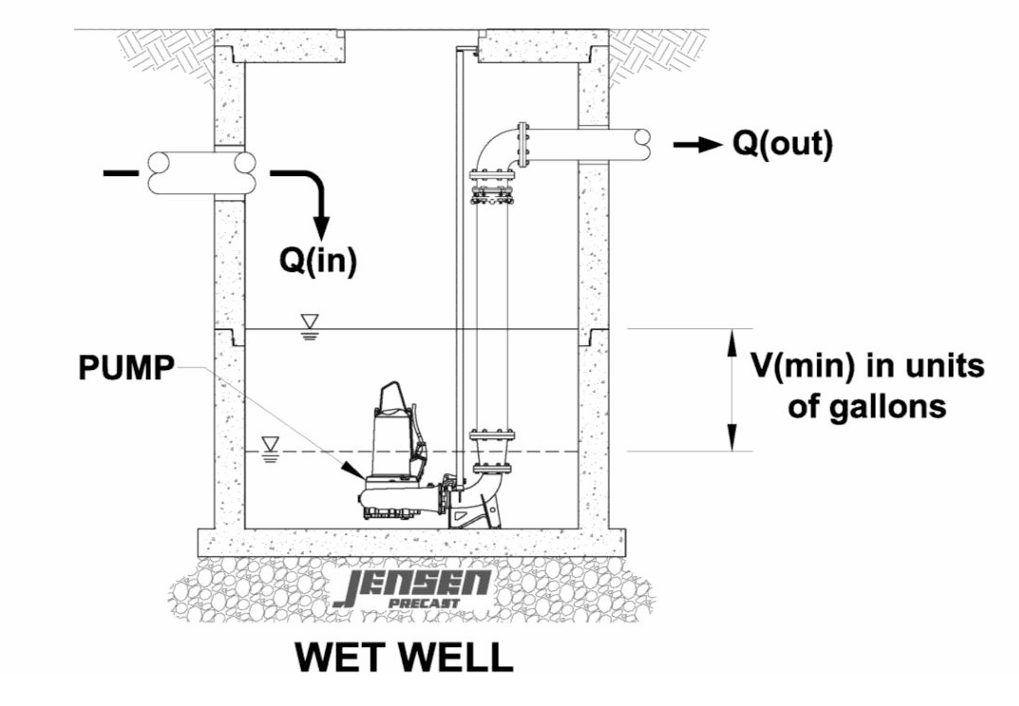
\includegraphics[
width=0.85\textwidth
]{calc_vmin.png}
\caption{Wet well storage and pumping configuration showing inflow, pump intake, and storage volume concept.\cite{Jensen_PumpStationDesignGuidelines_2012}}
\label{fig:wetwell_storage_config}
\end{figure}

As shown in Figure~\ref{fig:wetwell_storage_config}, the wet well receives an inflow of $12.46~\text{gpm}$ and the selected pump discharges at $135.50~\text{gpm}$, which creates the active storage and drawdown region used in the minimum storage calculation.

The design inflow rate to the wet well was determined from the projected wastewater flow for the subdivision, while the discharge rate corresponds to the operating point determined from the pump selection process. The resulting wet well configuration ensures reliable wastewater conveyance to the downstream gravity sewer system located at elevation $309.28~\text{ft}$, as illustrated in the system profile drawing \cite{ProjectD_Colebrooke_2020}.

% -------------------------------------------------
\subsection{Minimum Storage Volume}
% -------------------------------------------------

Wet well storage volume is designed to ensure that pumps do not start and stop excessively. Frequent pump cycling can cause increased mechanical wear, higher electrical loads, and reduced pump life. For low-flow lift stations, Jensen recommends sizing the wet well so that the time between pump starts is approximately $8$--$10$ minutes, while also verifying that the selected pump does not exceed the allowable number of starts per hour \cite{Jensen_PumpStationDesignGuidelines_2012}. The Sulzer pump data indicate a maximum of $15$ starts per hour, which corresponds to an absolute minimum interval of about $4$ minutes between starts. The selected design therefore satisfies the manufacturer limit if the cycle time is kept at $10$ minutes.

The minimum storage volume was calculated using the general Hydraulic Institute cycle-time relationship rather than the Jensen simplification $Q_{in}=Q_{out}/2$, because the actual inflow and selected pump discharge are already known for this project. Using the notation of the guideline, the cycle time is

\[
\begin{aligned}
T_{min} &= \frac{V_{min}}{Q_{in}} + \frac{V_{min}}{Q_{out}-Q_{in}}
\end{aligned}
\]

where $Q_{in}=12.46~\text{gpm}$, $Q_{out}=135.50~\text{gpm}$, and $T_{min}=10~\text{min}$.

First, the net pumping rate during pump operation is

\[
\begin{aligned}
Q_{out}-Q_{in} &= 135.50-12.46 \\
&= 123.04~\text{gpm}
\end{aligned}
\]

Substituting into the cycle-time equation gives

\[
\begin{aligned}
10 &= \frac{V_{min}}{12.46}+\frac{V_{min}}{123.04} \\
10 &= V_{min}\left(\frac{1}{12.46}+\frac{1}{123.04}\right) \\
10 &= V_{min}(0.08026+0.00813) \\
10 &= V_{min}(0.08839) \\
V_{min} &= \frac{10}{0.08839}=113.1~\text{gal}
\end{aligned}
\]

Thus, the minimum storage volume required to maintain a $10$-minute cycle time is

\[
\boxed{V_{min}=113~\text{gal}}
\]

This value, however, only satisfies the cycle-time requirement. A run-time check was then performed because a very small wet well volume can cause the pump to start and stop too quickly. The pump-on run time corresponding to $V_{min}=113~\text{gal}$ is

\[
\begin{aligned}
t_{on} &= \frac{V}{Q_{out}-Q_{in}} \\
&= \frac{113.1}{123.04}=0.919~\text{min}
\end{aligned}
\]

\[
\begin{aligned}
t_{on} &= 0.919\times 60 \\
&= 55.1~\text{s}
\end{aligned}
\]

A run time of $55.1~\text{s}$ is short for a submersible wastewater pump, even though the starts-per-hour criterion is technically met. In the absence of a stricter minimum run-time value from the manufacturer, a $2$-minute minimum run time was adopted as a conservative engineering design value for wet well sizing. Using this criterion, the required active storage becomes

\[
\begin{aligned}
V &= (Q_{out}-Q_{in})t_{on} \\
&= 123.04\times 2 \\
&= 246.08~\text{gal}
\end{aligned}
\]

For design purposes, this was rounded to

\[
\boxed{V_{min,\ design}=250~\text{gal}}
\]

Accordingly, the final wet well design volume was governed by the minimum run-time check rather than the $10$-minute cycle-time check. The selected design values used in the wet well figure are summarized in Figure~\ref{fig:wetwell_storage_volume}.

The wet well storage region used in this calculation is illustrated in Figure~\ref{fig:wetwell_storage_volume}.

\begin{figure}[H]
\centering
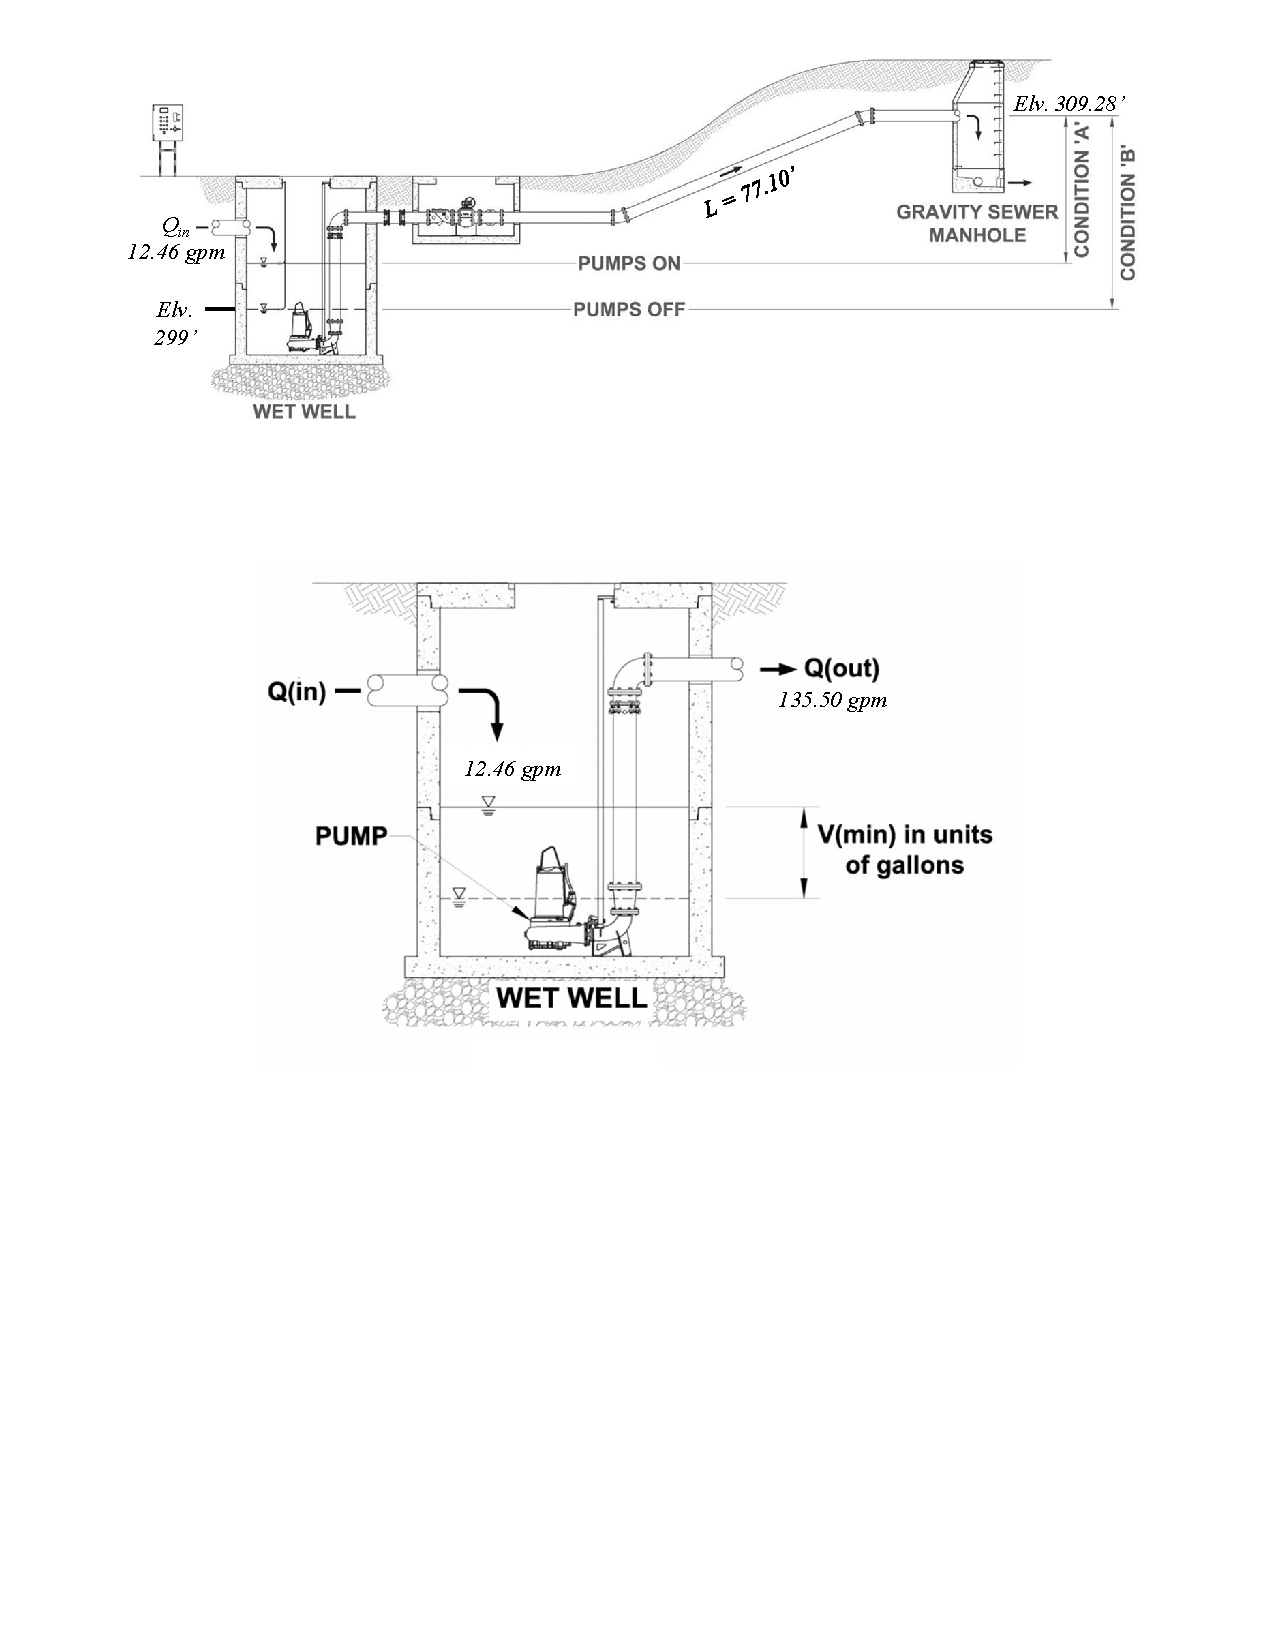
\includegraphics[
width=\textwidth,
trim={1.5in 4in 1.5in 4in},
clip
]{forcemain_pump_figures.pdf}
\caption{Wet well storage volume and inflow--outflow concept used for minimum storage calculations.}
\label{fig:wetwell_storage_volume}
\end{figure}

As shown in Figure~\ref{fig:wetwell_storage_volume}, the active storage region corresponds to the vertical distance between the pump-off and lead pump-on elevations within the wet well.

% -------------------------------------------------
\subsection{Hatch Sizing}
% -------------------------------------------------

After establishing the active storage requirement, the next step was to determine the minimum hatch opening needed for a duplex installation. The Sulzer installation dimension sheet for the XFP100C VX wet well installation shows that the recommended minimum opening for two pumps is $28~\text{in} \times 56~\text{in}$ on the U.S. dimension sheet, which was adopted directly for this design. The pump layout and minimum opening requirement are illustrated in Figure~\ref{fig:pump_install_dims}.

\begin{figure}[H]
\centering
\includegraphics[
width=0.9\textwidth,
page=2,
trim={0.2in 0.2in 0.2in 0.2in},
clip
]{dimension_ANM22624.pdf}
\caption{Installation dimensions for Sulzer XFP100C VX pump showing recommended hatch opening.}
\label{fig:pump_install_dims}
\end{figure}

As illustrated in Figure~\ref{fig:pump_install_dims}, the hatch opening must accommodate both pumps, their guide rail arrangement, lifting access, and the discharge hardware. The selected minimum hatch size for the wet well is therefore

\[
\boxed{28~\text{in} \times 56~\text{in}}
\]

This hatch dimension was not used by itself to select the wet well diameter. It was treated as the starting geometric requirement, and then the wet well diameter was checked against circular fit, pump clearances, and the discharge hardware inside the wet well.

Additional considerations for hatch design include loading classification, corrosion resistance, non-skid surfaces, and safety grates in accordance with industry practices \cite{Jensen_PumpStationDesignGuidelines_2012}.

% -------------------------------------------------
\subsection{Wet Well Diameter and Geometry}
% -------------------------------------------------

Most packaged lift stations utilize circular wet wells because round structures provide several advantages, including greater structural strength under soil pressure, lower construction cost, a smaller surface footprint, and simpler installation and precast manufacturing. A circular wet well was therefore selected for the Colebrooke station because round wet wells are standard for packaged duplex submersible lift stations and are structurally efficient for buried installation \cite{Jensen_PumpStationDesignGuidelines_2012}. Once the hatch size was known, the wet well diameter was evaluated. The first check was the geometric compatibility of the rectangular hatch with a circular wet well. The hatch diagonal is

\[
\begin{aligned}
d &= \sqrt{28^2+56^2} \\
&= \sqrt{784+3136} \\
&= \sqrt{3920} \\
&= 62.61~\text{in}
\end{aligned}
\]

Therefore, the wet well inside diameter must be greater than $62.61~\text{in}$ simply to accommodate the hatch geometry.

The next check was internal constructability. The selected pump is a DN100 unit with DN100 suction outlet and DN100 discharge outlet, which corresponds to a $4$-in connection. For a typical $4$-in flanged discharge connection, a reasonable working flange envelope of about $9~\text{in}$ outside diameter was assumed, with additional clearance required for the duckfoot elbow, guide rail connection, and contractor access for bolt tightening. The Sulzer installation sheet also shows a pump width of about $11.8~\text{in}$ in plan, and the discharge elbow and rail arrangement occupy additional horizontal space within the wet well. Because of this, selecting a wet well diameter only slightly larger than the hatch diagonal would leave insufficient room for the discharge elbow, flange, wall clearance, and maintenance access.

For that reason, the next standard practical diameter above the geometric minimum was adopted:

\[
\boxed{D_{well}=6~\text{ft ID}}
\]

This provides a $72$-in inside diameter, which exceeds the $62.61$-in hatch diagonal by

\[
\begin{aligned}
72-62.61 &= 9.39~\text{in}
\end{aligned}
\]

and also provides a workable margin for the $4$-in discharge hardware and wall clearances. This selection follows the same logic discussed in the Jensen guidance, namely that the hatch may geometrically fit but the well should be increased as needed to accommodate flanges, bends, and contractor working space \cite{Jensen_PumpStationDesignGuidelines_2012}. The selected $6$-ft-diameter well therefore represents a practical and constructible size rather than a purely geometric minimum.

% -------------------------------------------------
\subsection{Control Elevations}
% -------------------------------------------------

After determining the wet well size and minimum storage volume, the vertical control elevations that govern pump operation are established. In a duplex pumping system, five key control elevations are required:

\begin{enumerate}
\item Pump inlet elevation
\item Pump-off elevation
\item Lead pump-on elevation
\item Lag pump-on elevation
\item High water alarm elevation
\end{enumerate}

\begin{figure}[H]
\centering
\includegraphics[
width=\textwidth,
page=2,
trim={1.5in 2.5in 1in 4in},
clip
]{forcemain_pump_figures.pdf}
\caption{Wet well control elevations including pump-off, lead pump-on, lag pump-on, and high water alarm levels.}
\label{fig:wetwell_control_levels}
\end{figure}

As shown in Figure~\ref{fig:wetwell_control_levels}, the selected design values for the control increments are about $14~\text{in}$, $14.2~\text{in}$, $6~\text{in}$, and $12~\text{in}$ for $H_x$, $H_{min}$, $H_{lag}$, and $H_{res}$, respectively.

% -------------------------------------------------
\subsection{Minimum Submergence ($H_x$)}
% -------------------------------------------------

Once the wet well diameter and pump arrangement were fixed, the minimum submergence between the pump inlet and the pump-off water level was calculated to prevent vortex formation and air entrainment. Hydraulic Institute guidance provides empirical relationships for determining the required submergence based on pump inlet diameter and velocity \cite{ANSI_HI_98_1998,Hecker_1987_Conclusions}.

The minimum submergence relation from Hecker is

\[
\begin{aligned}
H_x &= D(1+2.3F_D)
\end{aligned}
\]

where

\[
\begin{aligned}
F_D &= \frac{V}{\sqrt{gD}}
\end{aligned}
\]

For the selected pump:

suction diameter $D=\text{DN100}=3.94~\text{in}=0.328~\text{ft}$
and pump discharge $Q=135.5~\text{gpm}$

Converting flow to cubic feet per second,

\[
\begin{aligned}
Q &= \frac{135.5}{448.83} \\
&= 0.302~\text{cfs}
\end{aligned}
\]

The suction area is

\[
\begin{aligned}
A &= \frac{\pi D^2}{4} \\
&= \frac{\pi(0.328)^2}{4} \\
&= 0.0845~\text{ft}^2
\end{aligned}
\]

The inlet velocity is

\[
\begin{aligned}
V &= \frac{Q}{A} \\
&= \frac{0.302}{0.0845} \\
&= 3.57~\text{ft/s}
\end{aligned}
\]

The hydraulic Froude number is

\[
\begin{aligned}
F_D &= \frac{3.57}{\sqrt{32.2(0.328)}} \\
&= \frac{3.57}{3.25} \\
&= 1.10
\end{aligned}
\]

Substituting into the submergence equation,

\[
\begin{aligned}
H_x &= 0.328(1+2.3\times 1.10) \\
&= 0.328(1+2.53) \\
&= 0.328(3.53) \\
&= 1.16~\text{ft}
\end{aligned}
\]

\[
\begin{aligned}
H_x &= 1.16\times 12 \\
&= 13.9~\text{in}
\end{aligned}
\]

Thus, the required minimum submergence is

\[
\boxed{H_x=14~\text{in}}
\]

The Sulzer installation dimension sheet indicates a water level dimension of $12.3~\text{in}$ for the selected installation arrangement. Because the calculated submergence requirement is larger, the design adopted the more conservative value of $14~\text{in}$.

% -------------------------------------------------
\subsection{Minimum Storage Depth ($H_{min}$)}
% -------------------------------------------------

The vertical distance between the pump-off elevation and the lead pump-on elevation is determined from the active wet well storage volume and wet well cross-sectional area. The governing design active storage was taken as $250~\text{gal}$. Converting this volume to cubic feet,

\[
\begin{aligned}
V &= 250\times 0.13368 \\
&= 33.42~\text{ft}^3
\end{aligned}
\]

For a $6$-ft-diameter circular wet well, the cross-sectional area is

\[
\begin{aligned}
A &= \pi r^2 \\
&= \pi(3)^2 \\
&= 28.27~\text{ft}^2
\end{aligned}
\]

Therefore,

\[
\begin{aligned}
H_{min} &= \frac{V}{A} \\
&= \frac{33.42}{28.27} \\
&= 1.18~\text{ft}
\end{aligned}
\]

\[
\begin{aligned}
H_{min} &= 1.18\times 12 \\
&= 14.2~\text{in}
\end{aligned}
\]

Thus, the required storage depth between pump-off and lead pump-on elevations is

\[
\boxed{H_{min}=14.2~\text{in}}
\]

% -------------------------------------------------
\subsection{Lag Pump Storage ($H_{lag}$)}
% -------------------------------------------------

For duplex stations with flows less than $200~\text{gpm}$, Jensen recommends a lag storage increment of at least $6~\text{in}$ \cite{Jensen_PumpStationDesignGuidelines_2012}. Since the selected pump discharge is $135.5~\text{gpm}$, the Colebrooke station falls within that range. Accordingly,

\[
\boxed{H_{lag}=6~\text{in}=0.5~\text{ft}}
\]

This is the vertical distance between the lead pump-on elevation and the lag pump-on elevation.

% -------------------------------------------------
\subsection{Reservoir Storage ($H_{res}$)}
% -------------------------------------------------

The reservoir storage between the lag pump-on elevation and the high water alarm is a factor of safety that provides emergency storage in the event of excessive inflow or pump malfunction. For small stations below $200~\text{gpm}$, Jensen recommends a minimum value of $12~\text{in}$ \cite{Jensen_PumpStationDesignGuidelines_2012}. Therefore,

\[
\boxed{H_{res}=12~\text{in}=1.0~\text{ft}}
\]

% -------------------------------------------------
\subsection{Summary of Wet Well Design Parameters}
% -------------------------------------------------

Based on the hydraulic calculations and equipment data, the recommended wet well configuration for the Colebrooke Subdivision pump station is summarized in Table~\ref{tab:wetwell_summary}.

\begin{table}[H]
\centering
\caption{Summary of recommended wet well design parameters}
\label{tab:wetwell_summary}
\begin{tabular}{ll}
\toprule
\textbf{Parameter} & \textbf{Value} \\
\midrule
Pump type & Sulzer XFP100C VX 1$\sim$ (wet pit) \\
Pump capacity & $135.5~\text{gpm}$ at $12.08~\text{ft}$ head \\
Impeller type & Vortex impeller \\
Wet well diameter & $6~\text{ft}$ inside diameter \\
Active storage volume & $250~\text{gal}$ \\
Minimum storage depth ($H_{min}$) & $14.2~\text{in}$ \\
Minimum submergence ($H_x$) & $14~\text{in}$ \\
Lag pump storage ($H_{lag}$) & $6~\text{in}$ \\
Reservoir storage ($H_{res}$) & $12~\text{in}$ \\
Recommended hatch opening & $28~\text{in} \times 56~\text{in}$ \\
\bottomrule
\end{tabular}
\end{table}

The selected control-elevation increments are

\[
H_x = 14~\text{in}, \qquad
H_{min} = 14.2~\text{in}, \qquad
H_{lag} = 6~\text{in}, \qquad
H_{res} = 12~\text{in}
\]

These design parameters ensure that the wet well provides sufficient hydraulic storage, safe pump operation, and reliable performance under both normal and peak flow conditions. The final configuration also satisfies regulatory design recommendations and operational guidelines for municipal wastewater lift stations \cite{MDEQ_DesignGuidance_2025,TenStates_RecommendedStandards_2014}.

\newpage
% =================================================
% Chapter 6 — Final System Design and Design Summary
% =================================================

\section{Final System Design and Design Summary}

% -------------------------------------------------
\subsection{Final System Design}
% -------------------------------------------------

Following completion of the hydraulic analysis, pump selection, and wet well sizing, the wastewater conveyance system for the Colebrooke Subdivision is finalized as an integrated lift station and force main arrangement. The system consists of a duplex submersible pump station discharging through a short pressurized force main to the existing municipal gravity sewer manhole located along Lewis Street. The proposed pump station location, force main alignment, and downstream sewer connection were established using the subdivision survey and layout information \cite{ProjectD_Colebrooke_2020}.

The final arrangement of the pump station and force main is shown in Figure~\ref{fig:final_forcemain_layout}.

\begin{figure}[H]
\centering
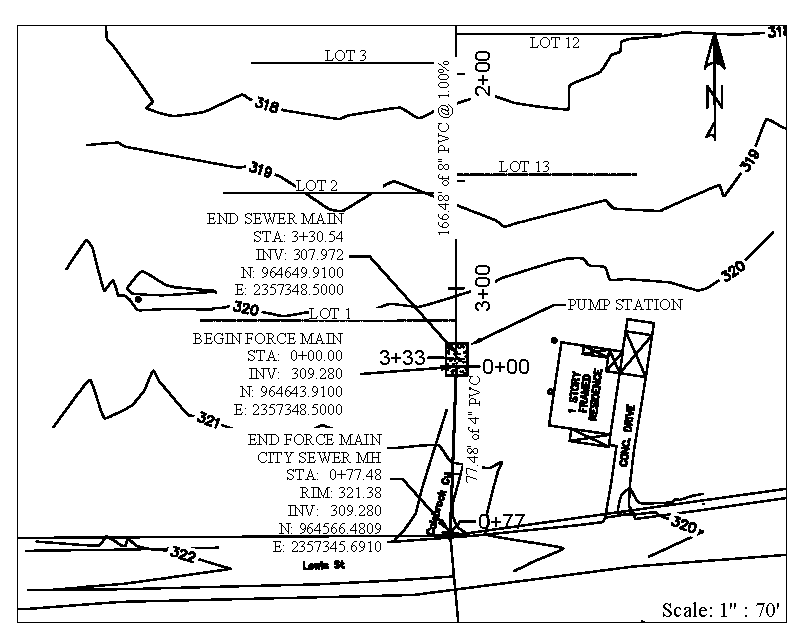
\includegraphics[
width=\textwidth
]{ForcemainLayoutPlan.pdf}
\caption{Final force main layout plan showing pump station location, 4-in force main alignment, and discharge connection to the existing city sewer manhole.}
\label{fig:final_forcemain_layout}
\end{figure}

As illustrated in Figure~\ref{fig:final_forcemain_layout}, the force main begins at the proposed pump station at Sta.~0+00.00 and extends approximately $77.48~\text{ft}$ to the existing municipal manhole at Sta.~0+77.48. The pump station coordinates are $N=964649.9100$, $E=2357348.5000$, and the receiving city sewer manhole is located at $N=964566.4809$, $E=2357345.6910$. Wastewater discharged from the pump enters the municipal gravity system at invert elevation $309.280~\text{ft}$.

The hydraulic relationship between the wet well and the receiving sewer is illustrated in Figure~\ref{fig:forcemain_profile}.

\begin{figure}[H]
\centering
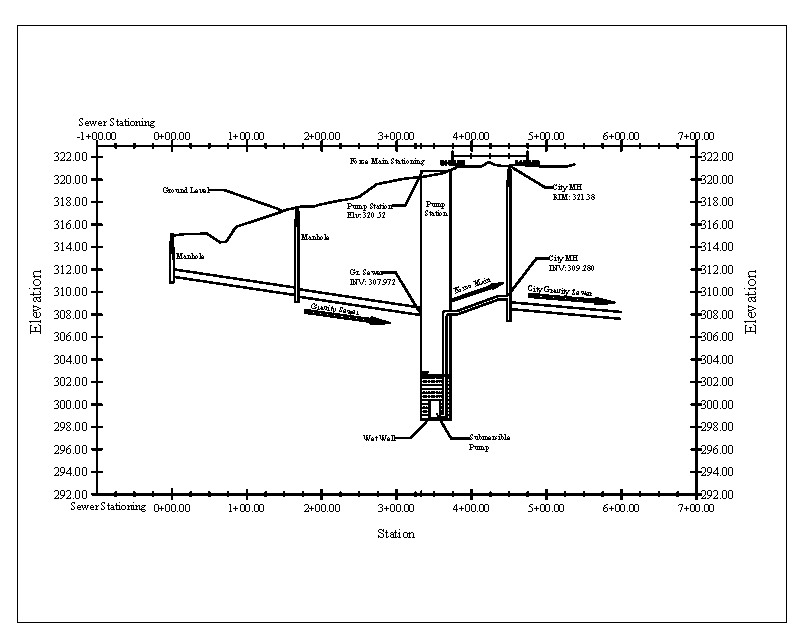
\includegraphics[
width=\textwidth
]{ForceMainLayoutProfile.pdf}
\caption{Final hydraulic profile showing the wet well, force main, and receiving city gravity sewer manhole.}
\label{fig:forcemain_profile}
\end{figure}

As shown in Figure~\ref{fig:forcemain_profile}, the wet well operating level is $299.00~\text{ft}$, while the receiving sewer invert is $309.280~\text{ft}$, producing a static head of $10.28~\text{ft}$. The profile confirms the short pressurized reach between the pump station and the municipal sewer connection and establishes the final vertical relationship between the wet well, ground surface, and discharge location.

% -------------------------------------------------
\subsection{Force Main Final Size Verification}
% -------------------------------------------------

The final force main diameter adopted for the system is $4$-in PVC pressure pipe. This size was selected after evaluating potential pipe diameters and confirming compliance with velocity, headloss, and regulatory requirements. Although the subdivision inflow is relatively small ($12.46~\text{gpm}$), wastewater lift stations using submersible pumps typically require a minimum $4$-in force main diameter except in grinder pump applications.

The final verification was performed using the selected pump operating point rather than the raw sewer inflow. The selected Sulzer XFP100C VX pump operates at $135.5~\text{gpm}$ and $12.08~\text{ft}$ of head according to the manufacturer performance curve. Using the pipe cross-sectional area of approximately $0.09~\text{ft}^2$, the resulting operating velocity is

\[
Q = 135.5~\text{gpm} = \frac{135.5}{448.83} = 0.302~\text{cfs}
\]

\[
V = \frac{Q}{A} = \frac{0.302}{0.09} = 3.36~\text{ft/s}
\]

\[
V \approx 3.4~\text{ft/s}
\]

This velocity exceeds the minimum wastewater transport velocity of $2~\text{ft/s}$ and falls within the commonly recommended $3$--$9~\text{ft/s}$ range for wastewater force mains. The value is sufficiently high to prevent solids deposition while remaining low enough to limit excessive headloss and pipe wear.

The total dynamic head corresponding to the selected pump operating point is $12.08~\text{ft}$, only slightly greater than the static head of $10.28~\text{ft}$, confirming that friction and minor losses remain small due to the short pipeline length and smooth PVC pipe surface.

The final force main configuration is therefore confirmed as

\[
\boxed{\text{4-in PVC force main, } L = 77.48~\text{ft}}
\]

% -------------------------------------------------
\subsection{Pump Station Configuration}
% -------------------------------------------------

The finalized lift station is configured as a duplex submersible sewage pumping station. The selected pump model is the Sulzer XFP100C VX 1$\sim$ (wet pit) equipped with a PE18/4W motor. The pump operates at $135.5~\text{gpm}$ and $12.08~\text{ft}$ of head, with a vortex impeller, DN100 suction outlet, DN100 discharge outlet, $3.94$-in free solids passage, and $2.414~\text{hp}$ motor output.

Two identical pumps are installed in the wet well. Under normal conditions one pump operates as the duty pump, while the second pump remains on standby. The standby pump provides redundancy and can automatically start if the inflow exceeds the capacity of a single pump or if the duty pump becomes unavailable. This configuration improves reliability and is standard practice for small municipal wastewater lift stations.

The selected pump uses a vortex impeller, which allows solids and fibrous material to pass through the pump casing without direct contact with the impeller vanes. This configuration improves clogging resistance for residential wastewater systems. The manufacturer data indicate a $3.94$-in free passage, which exceeds the typical $3$-in solids-handling requirement commonly used in wastewater pump selection.

% -------------------------------------------------
\subsection{Pump Station Control Levels}
% -------------------------------------------------

Once the wet well diameter and storage volume were determined, the control elevations governing pump operation were established. The control hierarchy consists of minimum submergence, active storage depth, lag-pump storage, and reservoir storage.

The finalized control elevation arrangement is illustrated in Figure~\ref{fig:final_wetwell_levels}.

\begin{figure}[H]
\centering
\includegraphics[
width=\textwidth,
page=2,
trim={1.5in 2.5in 1in 4in},
clip
]{forcemain_pump_figures.pdf}
\caption{Wet well control elevations showing minimum submergence, storage depth, lag pump activation, and high-water alarm levels.}
\label{fig:final_wetwell_levels}
\end{figure}

As shown in Figure~\ref{fig:final_wetwell_levels}, the final control increments are

\begin{enumerate}
\item Minimum submergence ($H_x = 14$ in)
\item Pump-off to lead-pump-on storage ($H_{min} = 14.2$ in)
\item Lead-pump-on to lag-pump-on storage ($H_{lag} = 6$ in)
\item Lag-pump-on to high-water alarm storage ($H_{res} = 12$ in)
\end{enumerate}

The minimum submergence between the pump inlet and pump-off water level was determined using the Hecker relation

\[
H_x = D(1+2.3F_D)
\]

with

\[
F_D = \frac{V}{\sqrt{gD}}
\]

Using the DN100 suction diameter and the pump operating flow, the required submergence was calculated as

\[
H_x = 13.9~\text{in} \approx 14~\text{in}
\]

The active storage depth was determined from the selected wet well storage volume of $250~\text{gal}$ and a $6$-ft diameter wet well, giving a cross-sectional area of $28.27~\text{ft}^2$. Converting storage volume to cubic feet,

\[
V = 250(0.13368) = 33.42~\text{ft}^3
\]

\[
H_{min} = \frac{V}{A} = \frac{33.42}{28.27} = 1.18~\text{ft} = 14.2~\text{in}
\]

These values establish the final pump control elevations summarized in Table~\ref{tab:control_levels}.

\begin{table}[H]
\centering
\caption{Final wet well control elevations}
\label{tab:control_levels}
\begin{tabular}{lc}
\toprule
Control increment & Value \\
\midrule
Minimum submergence ($H_x$) & 14 in \\
Pump-off to lead-pump-on ($H_{min}$) & 14.2 in \\
Lead-pump-on to lag-pump-on ($H_{lag}$) & 6 in \\
Lag-pump-on to high-water alarm ($H_{res}$) & 12 in \\
\bottomrule
\end{tabular}
\end{table}

% -------------------------------------------------
\subsection{Accessories and Mechanical Components}
% -------------------------------------------------

In addition to the pumps themselves, several mechanical components are required to support installation, maintenance, and operation of the lift station. These include guide rails, duckfoot discharge elbows, discharge piping, valves, and access openings.

The installation arrangement for the selected pump is illustrated in Figure~\ref{fig:sulzer_install}.

\begin{figure}[H]
\centering
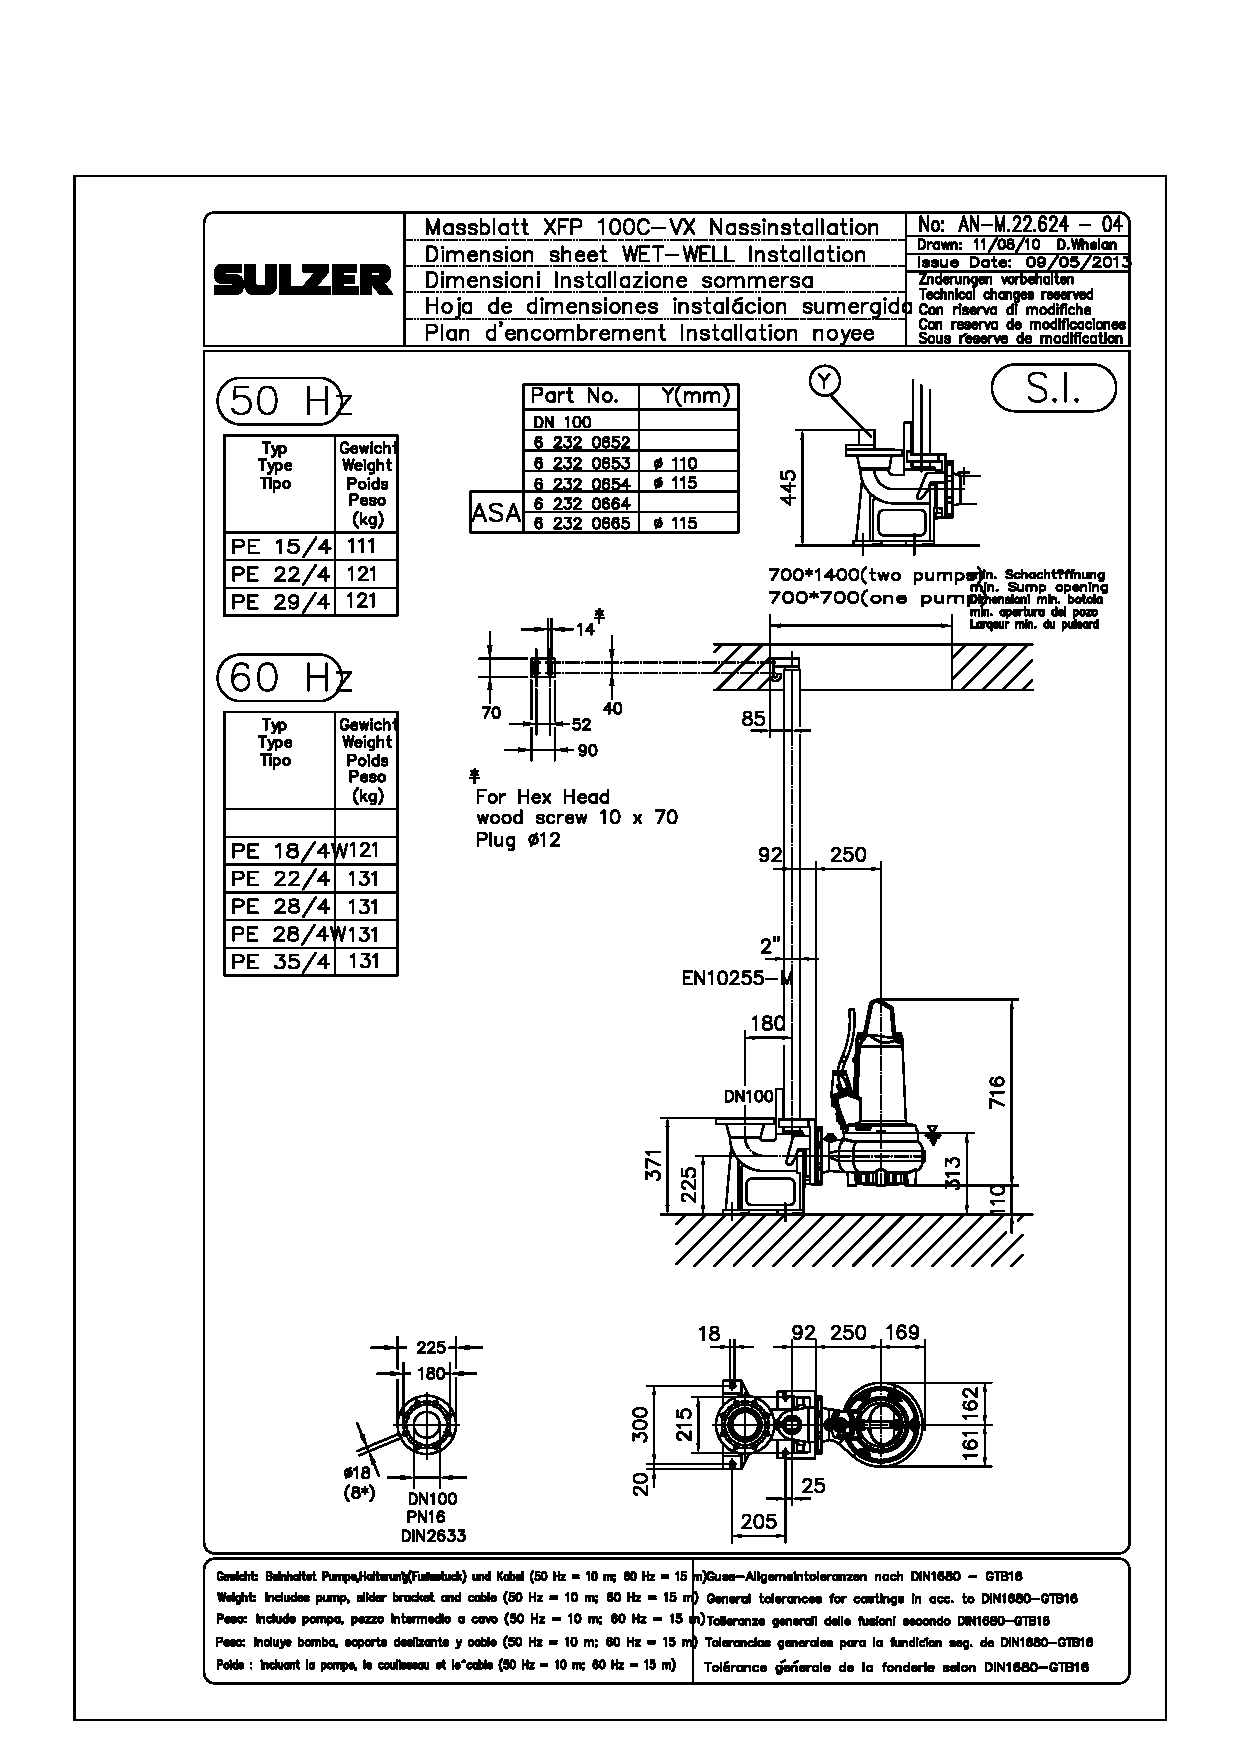
\includegraphics[
width=0.9\textwidth
]{dimension_ANM22624.pdf}
\caption{Sulzer XFP100C VX wet well installation arrangement showing duplex hatch opening, guide rail system, and discharge connection details.}
\label{fig:sulzer_install}
\end{figure}

Each pump is mounted on a guide rail system that allows removal and reinstallation from the ground surface without entering the wet well. The pumps connect to duckfoot discharge elbows at the base of the wet well, directing flow into the vertical discharge piping.

The manufacturer installation sheet indicates a recommended duplex hatch opening of $28~\text{in} \times 56~\text{in}$, which was adopted in the wet well design. The installation drawing also confirms the use of $4$-in Class 125 ANSI discharge hardware associated with the DN100 pump connection.

The discharge piping includes both a check valve and gate valve. The check valve prevents reverse flow when pump operation stops, while the gate valve allows isolation of the discharge piping during maintenance. Additional station components include lifting chains, level sensors, electrical power connections, and control equipment necessary for automatic pump operation.

% -------------------------------------------------
\subsection{Final Design Summary}
% -------------------------------------------------

The final design for the Colebrooke Subdivision lift station integrates the subdivision gravity sewer system with the existing municipal sewer network through a short pressurized force main and duplex wet well pump station. Wastewater collected from the subdivision flows to the wet well at a peak rate of $12.46~\text{gpm}$ and is pumped through a $4$-in PVC force main approximately $77.48~\text{ft}$ in length to the existing city sewer manhole at invert elevation $309.280~\text{ft}$ \cite{ProjectD_Colebrooke_2020}.

The selected pump is the Sulzer XFP100C VX 1$\sim$ (wet pit) with vortex impeller, operating at $135.5~\text{gpm}$ and $12.08~\text{ft}$ of head with $1.765~\text{hp}$ shaft power and $2.414~\text{hp}$ motor output. The wet well is designed as a $6$-ft inside diameter circular structure with $250~\text{gal}$ active storage, providing adequate storage and stable pump cycling.

The key design parameters are summarized in Table~\ref{tab:design_summary}.

\begin{table}[H]
\centering
\caption{Final system design summary}
\label{tab:design_summary}
\begin{tabular}{lc}
\toprule
Item & Final design \\
\midrule
Peak wastewater inflow & 12.46 gpm \\
Selected pump model & Sulzer XFP100C VX \\
Pump operating flow & 135.5 gpm \\
Pump operating head & 12.08 ft \\
Impeller type & Vortex \\
Free passage & 3.94 in \\
Motor output & 2.414 hp \\
Force main material & PVC pressure pipe \\
Force main diameter & 4 in \\
Force main length & 77.48 ft \\
Static head & 10.28 ft \\
Total dynamic head & 12.08 ft \\
Wet well diameter & 6 ft \\
Active wet well storage & 250 gal \\
Hatch opening & 28 in $\times$ 56 in \\
$H_x$ & 14 in \\
$H_{min}$ & 14.2 in \\
$H_{lag}$ & 6 in \\
$H_{res}$ & 12 in \\
\bottomrule
\end{tabular}
\end{table}

The final design satisfies the hydraulic requirements of the subdivision and provides adequate solids-handling capability and operational reliability. The selected pump, wet well, and force main operate as an integrated system consistent with the project layout and manufacturer installation requirements \cite{ProjectD_Colebrooke_2020}.

\newpage
% --------------------------------------------
% Slight Modification Needed file
% --------------------------------------------

\chapter{Cost Estimation}

\section{Cost Estimation Approach}

The cost estimate was developed using a unit cost–based methodology aligned with the finalized design of the lift station and force main system. Construction costs were derived from a combination of regional data sources, including Mississippi Department of Transportation (MDOT) bid price databases, recent municipal bid tabulations, and published cost references such as RSMeans. Where applicable, costs were adjusted to reflect the project scale, material specifications, and local construction conditions.

Major equipment costs, particularly the selected pump system, were estimated using vendor-based pricing for comparable configurations. Lump-sum values were adopted for components where detailed quantity breakdowns were not necessary at this stage. The estimate incorporates direct construction costs, indirect costs, and engineering-related expenses, along with appropriate allowances for contractor overhead, profit, and contingency, consistent with standard engineering practice and FHWA cost estimating guidance.

\section{Cost Breakdown}

\subsection{Direct Costs}

Direct construction costs represent the primary expenses associated with physically building the lift station and force main system. These costs include materials, labor, and equipment required for installation of structural components, mechanical systems, piping, and sitework. Unit costs were developed using regional bid data from the Mississippi Department of Transportation (MDOT), recent municipal project bid tabulations, and standard construction cost references, with adjustments made to reflect project-specific conditions and scale \cite{MDOT_BidTab_2024, CityMagnolia_BidTab_2024, CityClinton_BidTab_2020, RSMeans_CostData_2025}. Additional market-based pricing for pump station components and wastewater system infrastructure was verified using vendor and municipal cost references to ensure consistency with current construction practices \cite{ExcelFluidGroup_PumpComparison_2024, WaterLevelControls_LiftStationCosts_2024, Wildwood_UtilityCostSchedule_2022}.

\begin{table}[H]
\centering
\caption{Direct Construction Costs}
\label{tab:direct_costs}
\begin{adjustbox}{width=\textwidth}
\begin{tabular}{c l c c c c}
\toprule
\textbf{Item No.} & \textbf{Description} & \textbf{Qty} & \textbf{Unit} & \textbf{Unit Cost (\$)} & \textbf{Line Cost (\$)} \\
\midrule
1  & Sulzer XFP100C VX pumps & 2 & EA & 6,881.22 & 13,762.44 \\
2  & Precast concrete wet well (6-ft dia, 18–20 ft depth) & 1 & LS & 55,000.00 & 55,000.00 \\
3  & Valve vault and discharge assembly & 1 & LS & 22,000.00 & 22,000.00 \\
4  & Discharge piping system, guide rails, fittings & 1 & LS & 14,000.00 & 14,000.00 \\
5  & Check valve and gate valve (4-in) & 1 & LS & 6,500.00 & 6,500.00 \\
6  & Electrical and control system (panel, sensors, wiring) & 1 & LS & 38,000.00 & 38,000.00 \\
7  & Wet well protective coating & 1 & LS & 8,000.00 & 8,000.00 \\
8  & Site excavation, backfill, grading, yard piping & 1 & LS & 22,000.00 & 22,000.00 \\
9  & Access pad / gravel surface / minor site improvements & 1 & LS & 8,000.00 & 8,000.00 \\
10 & Erosion and sediment control & 1 & LS & 4,000.00 & 4,000.00 \\
11 & Quick-connect bypass assembly & 1 & LS & 5,500.00 & 5,500.00 \\
12 & 4-in PVC C900 DR18 force main & 80 & LF & 40.00 & 3,200.00 \\
13 & Trench bedding, backfill, and restoration & 80 & LF & 20.00 & 1,600.00 \\
14 & Force main fittings, tracer wire, markers & 1 & LS & 3,500.00 & 3,500.00 \\
15 & Connection to existing manhole & 1 & LS & 2,500.00 & 2,500.00 \\
16 & Traffic control & 1 & LS & 2,500.00 & 2,500.00 \\
\midrule
\multicolumn{5}{r}{\textbf{Direct Cost Subtotal}} & \textbf{210,062.44} \\
\bottomrule
\end{tabular}
\end{adjustbox}
\end{table}

\subsection{Indirect Costs}

Indirect costs represent supporting construction expenses that are not directly tied to specific quantities of installed work but are necessary for successful project execution. These include site preparation, temporary facilities, utility coordination, and mobilization and demobilization activities required to initiate and complete construction operations. The adopted values were developed based on regional bid tabulations and typical municipal construction practices, with reference to MDOT cost data and recent project bid summaries \cite{MDOT_BidTab_2024, CityMagnolia_BidTab_2024, CertifiedBidTab_Provided_2024}.


\begin{table}[H]
\centering
\caption{Indirect Costs}
\label{tab:indirect_costs}
\begin{tabular}{c l c c c c}
\toprule
17 & Site preparation              & 1 & LS & 6,000.00  & 6,000.00  \\
18 & Temporary facilities          & 1 & LS & 4,000.00  & 4,000.00  \\
19 & Utilities allowance           & 1 & LS & 3,500.00  & 3,500.00  \\
20 & Mobilization / demobilization & 1 & LS & 15,000.00 & 15,000.00 \\
\midrule
\multicolumn{5}{r}{\textbf{Indirect Cost Subtotal}} & \textbf{28,500.00} \\
\bottomrule
\end{tabular}
\end{table}


\subsection{Engineering and Design Costs}

Engineering and design costs include professional services required for planning, investigation, and development of the wastewater conveyance system. These costs consist of surveying for site layout and alignment, geotechnical investigation for subsurface characterization, and design and consulting services for hydraulic, structural, and system design. The values were estimated based on typical ranges observed in municipal infrastructure projects and standard engineering practice, with reference to published cost data and planning-level estimates \cite{CityClinton_ArrowDrive_2025, RSMeans_CostData_2025, FHWA_MajorProjectCostGuidance_2007}.

\begin{table}[H]
\centering
\caption{Engineering and Design Costs}
\label{tab:engineering_costs}
\begin{tabular}{c l c c c c}
\toprule
21 & Surveying                  & 1 & LS & 4,000.00  & 4,000.00  \\
22 & Geotechnical investigation & 1 & LS & 6,000.00  & 6,000.00  \\
23 & Design and consulting fees & 1 & LS & 18,000.00 & 18,000.00 \\
\midrule
\multicolumn{5}{r}{\textbf{Engineering \& Design Subtotal}} & \textbf{28,000.00} \\
\bottomrule
\end{tabular}
\end{table}

\subsection{Overhead, Profit, and Contingency}

Additional project costs include contractor overhead, profit, and contingency allowances, which are applied to the combined direct and indirect construction costs. Contractor overhead accounts for administrative expenses, insurance, and general project management requirements, while profit represents the contractor’s return for undertaking the work. A contingency allowance is included to account for uncertainties associated with material prices, construction conditions, and minor design variations. The selected percentages are consistent with typical ranges recommended in engineering practice and federal cost estimating guidance \cite{FHWA_MajorProjectCostGuidance_2007, RSMeans_CostData_2025}.

\begin{table}[H]
\centering
\caption{Cost Adders: Overhead, Profit, and Contingency}
\label{tab:adders}
\begin{tabular}{l c c c}
\toprule
\textbf{Category} & \textbf{Basis} & \textbf{Rate} & \textbf{Amount (\$)} \\
\midrule
Contractor Overhead & Direct + Indirect & 7\%  & 16,699.37 \\
Contractor Profit   & Direct + Indirect & 7\%  & 16,699.37 \\
Contingency         & Direct + Indirect & 10\% & 23,856.24 \\
\bottomrule
\end{tabular}
\end{table}

\section{Total Project Cost}

The total project cost was determined by combining direct construction costs, indirect costs, engineering and design costs, and applicable contractor adders, including overhead, profit, and contingency. This comprehensive estimate reflects the finalized system design and incorporates all major cost components required for project implementation. The inclusion of contingency and contractor-related costs ensures that the estimate accounts for potential variability in construction conditions and market factors, consistent with standard engineering cost estimation practices \cite{FHWA_MajorProjectCostGuidance_2007}.

\begin{table}[H]
\centering
\caption{Total Project Cost Summary}
\label{tab:total_cost}
\begin{tabular}{l c}
\toprule
\textbf{Category} & \textbf{Amount (\$)} \\
\midrule
Direct Construction Costs & 210,062.44 \\
Indirect Costs            & 28,500.00  \\
Engineering \& Design     & 28,000.00  \\
Contractor Overhead       & 16,699.37  \\
Contractor Profit         & 16,699.37  \\
Contingency               & 23,856.24  \\
\midrule
\textbf{Total Project Cost} & \textbf{323,817.42} \\
\bottomrule
\end{tabular}
\end{table}


\section{Chapter Summary}

The final cost estimate for the proposed wastewater lift station and force main system is based on the finalized hydraulic and layout configuration of the selected design. The proposed system consists of a duplex lift station and an 80-ft-long 4-in PVC force main discharging to the existing municipal sewer system. Using regional bid data, standard cost references, and vendor-based pricing, the estimate was developed to reflect current construction conditions and the major cost components required for implementation \cite{MDOT_BidTab_2024, CityMagnolia_BidTab_2024, CityClinton_BidTab_2020, RSMeans_CostData_2025, FHWA_MajorProjectCostGuidance_2007, Shifat_CostEstimate_2026}.

Direct construction costs constitute the largest share of the budget, totaling \$210{,}062.44. Within this category, the precast concrete wet well, electrical and control system, valve vault and discharge assembly, and excavation-related work represent the dominant cost items. Indirect costs total \$28{,}500.00, while engineering and design costs total \$28{,}000.00. Contractor overhead and profit were each applied at 7\% of the combined direct and indirect construction costs, resulting in \$16{,}699.37 each, and a 10\% contingency allowance was included in the amount of \$23{,}856.24 \cite{Shifat_CostEstimate_2026}.

The distribution of contractor overhead, profit, and contingency is shown in Figure~\ref{fig:adders}. The overall comparison of major project cost components is shown in Figure~\ref{fig:cost_breakdown}. Based on the corrected final estimate, the total project cost is \$323{,}817.42 \cite{Shifat_CostEstimate_2026}. This value represents the full planning-level estimate for the proposed system and provides a practical basis for budgeting and future project development.

\begin{figure}[H]
\centering
\includegraphics[width=0.8\textwidth]{figures/adders.png}
\caption{Distribution of Cost Adders}
\label{fig:adders}
\end{figure}

\begin{figure}[H]
\centering
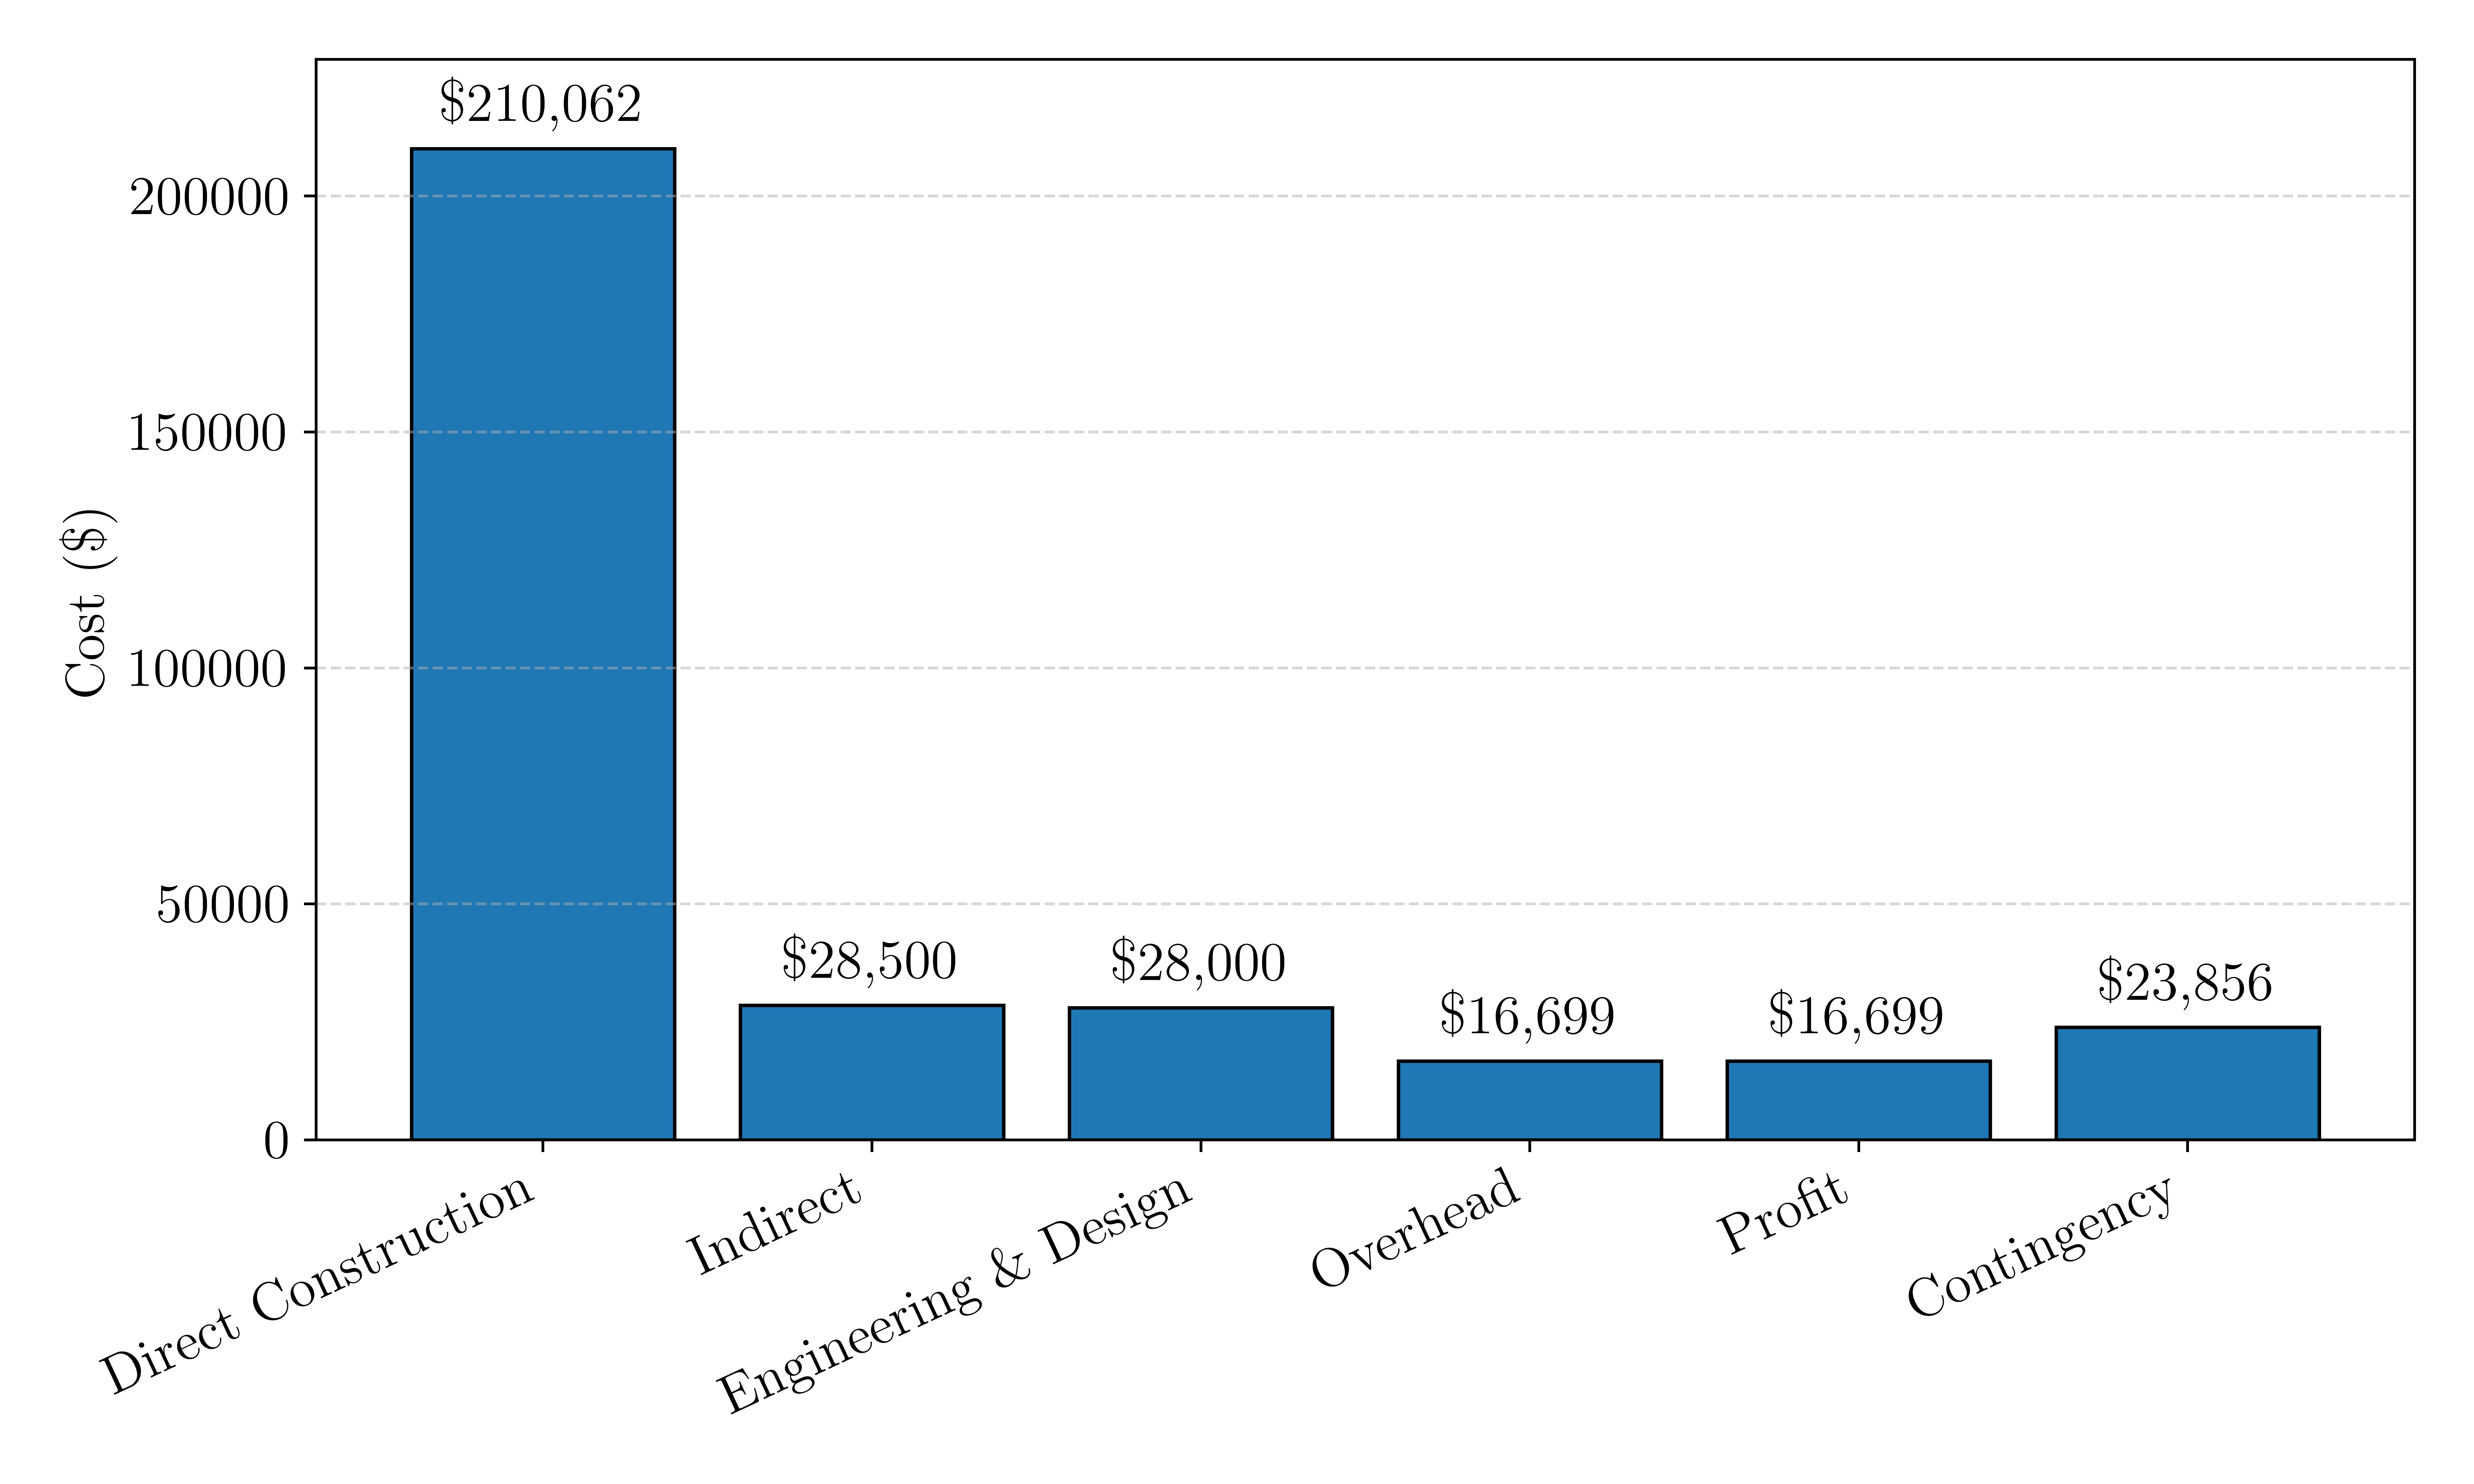
\includegraphics[width=\textwidth]{figures/costing.png}
\caption{Summary of Major Cost Components for the Proposed Lift Station System}
\label{fig:cost_breakdown}
\end{figure}

\newpage
% \section*{References}
\printbibliography[heading=bibintoc,title={References}]

% Mississippi Department of Environmental Quality (MDEQ). \textit{Guidance for the Design of Publicly Owned Wastewater Facilities.} Jackson, MS.

% Project D -- Subdivision. (2020). \textit{Colebrooke Subdivision Design Report.} Florence, Mississippi.

% Geotechnical Report -- Colebrooke Subdivision. (2022). \textit{Subsurface Investigation and Soil Evaluation for Proposed Residential Development.}

% Ten States Standards. (2014). \textit{Recommended Standards for Wastewater Facilities.} Great Lakes -- Upper Mississippi River Board.

% Romtec Utilities. \textit{Standard Duplex Lift Station Assembly Diagram.} Retrieved from \url{https://romtecutilities.com}

% Smith Pump Company. \textit{Duplex Submersible Lift Station Plan and Section Drawing.}

% Cape Fear Public Utility Authority (CFPUA). \textit{Residential Grinder Pump Connection Diagram.} Retrieved from \url{https://www.cfpua.org}

% Lakeside Municipal Utility District. \textit{Low-Pressure Grinder Pump Sewer Layout Diagram.}

% Frederick County Division of Utilities and Solid Waste Management. \textit{Grinder Pump and Gravity Flow Connection Illustration.}

% Sewer Engineering Illustration (Public Domain). \textit{Cross-Section of Gravity Sewer System Showing Manhole and Main Alignment.}

\clearpage
\appendix
\addcontentsline{toc}{chapter}{Appendix}

% Appendix A
\renewcommand{\thesection}{A.\arabic{section}}
\setcounter{section}{0}
\setcounter{figure}{0}
\renewcommand{\thefigure}{A.\arabic{figure}}

\section{Preliminary Plat}
\begin{figure}[H]
\centering
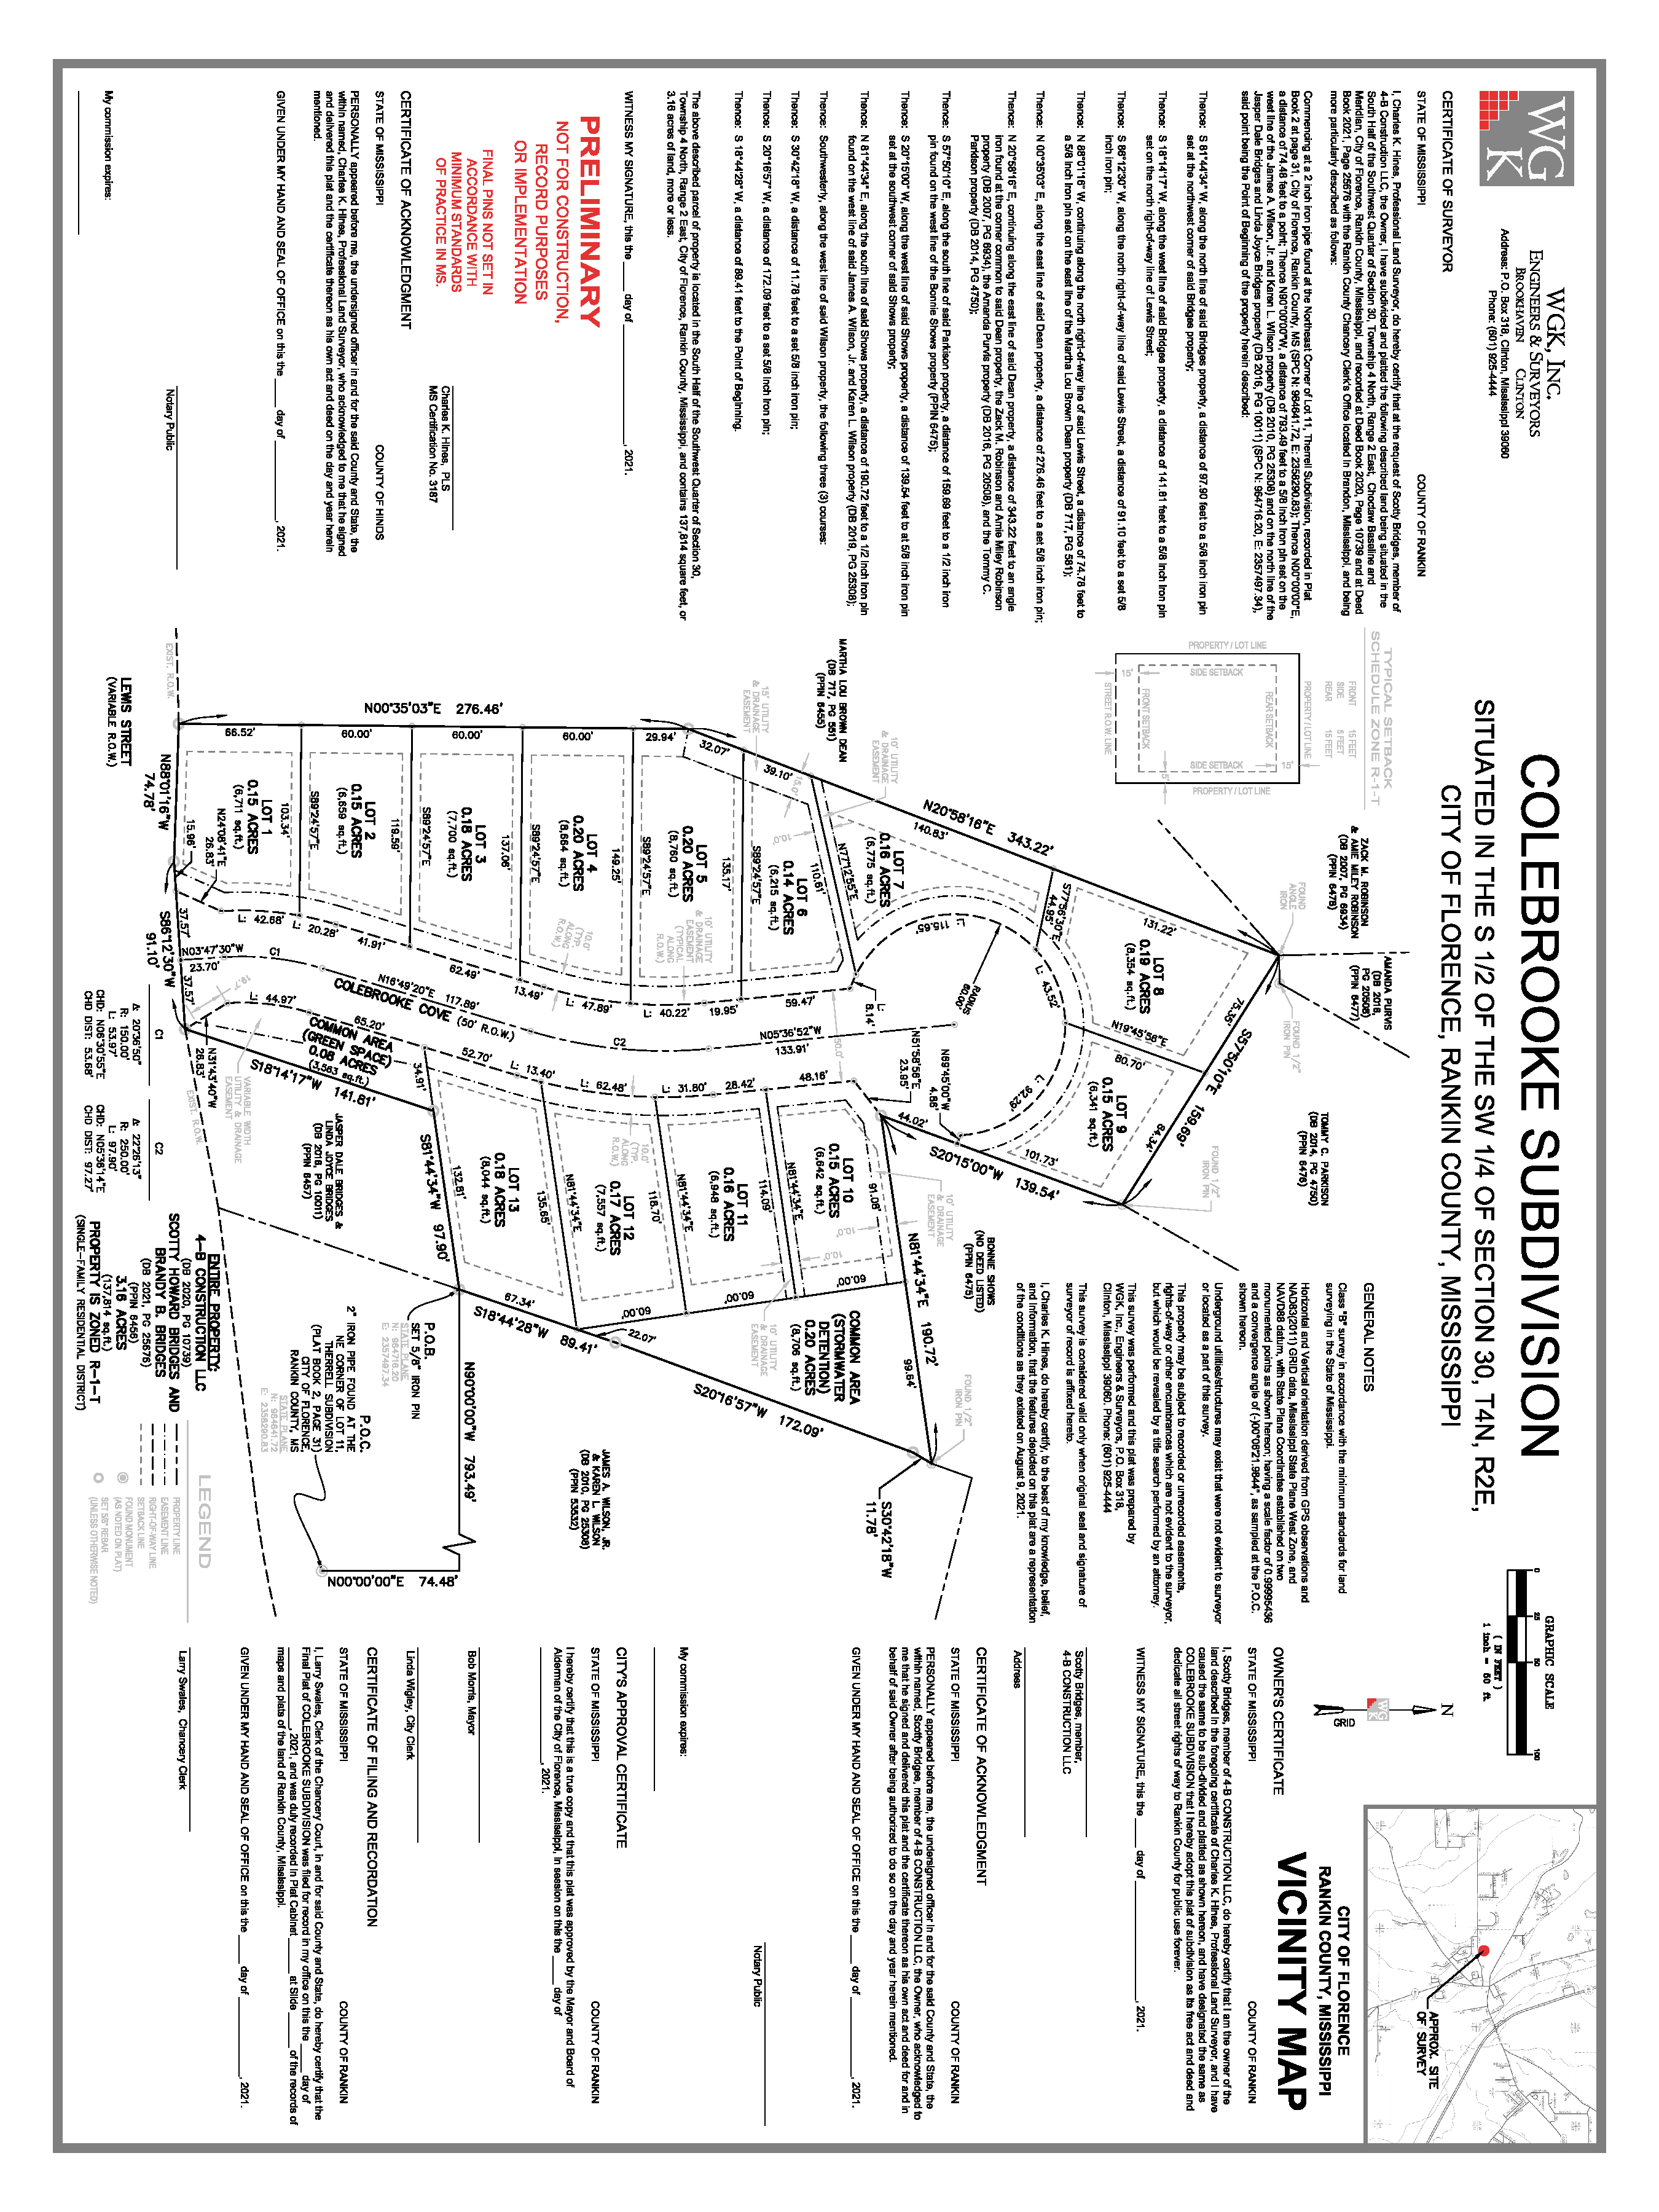
\includegraphics[
width=\textwidth,
]{./subdivision_plat_Prelim Plat_Colebrooke Subdivsion (1) (1).pdf}
\end{figure}



% Appendix B
\renewcommand{\thesection}{B.\arabic{section}}
\setcounter{section}{0}
\setcounter{figure}{0}
\renewcommand{\thefigure}{B.\arabic{figure}}

\section{XFP100C VX1 Data Sheet}
\begin{figure}[H]
\centering
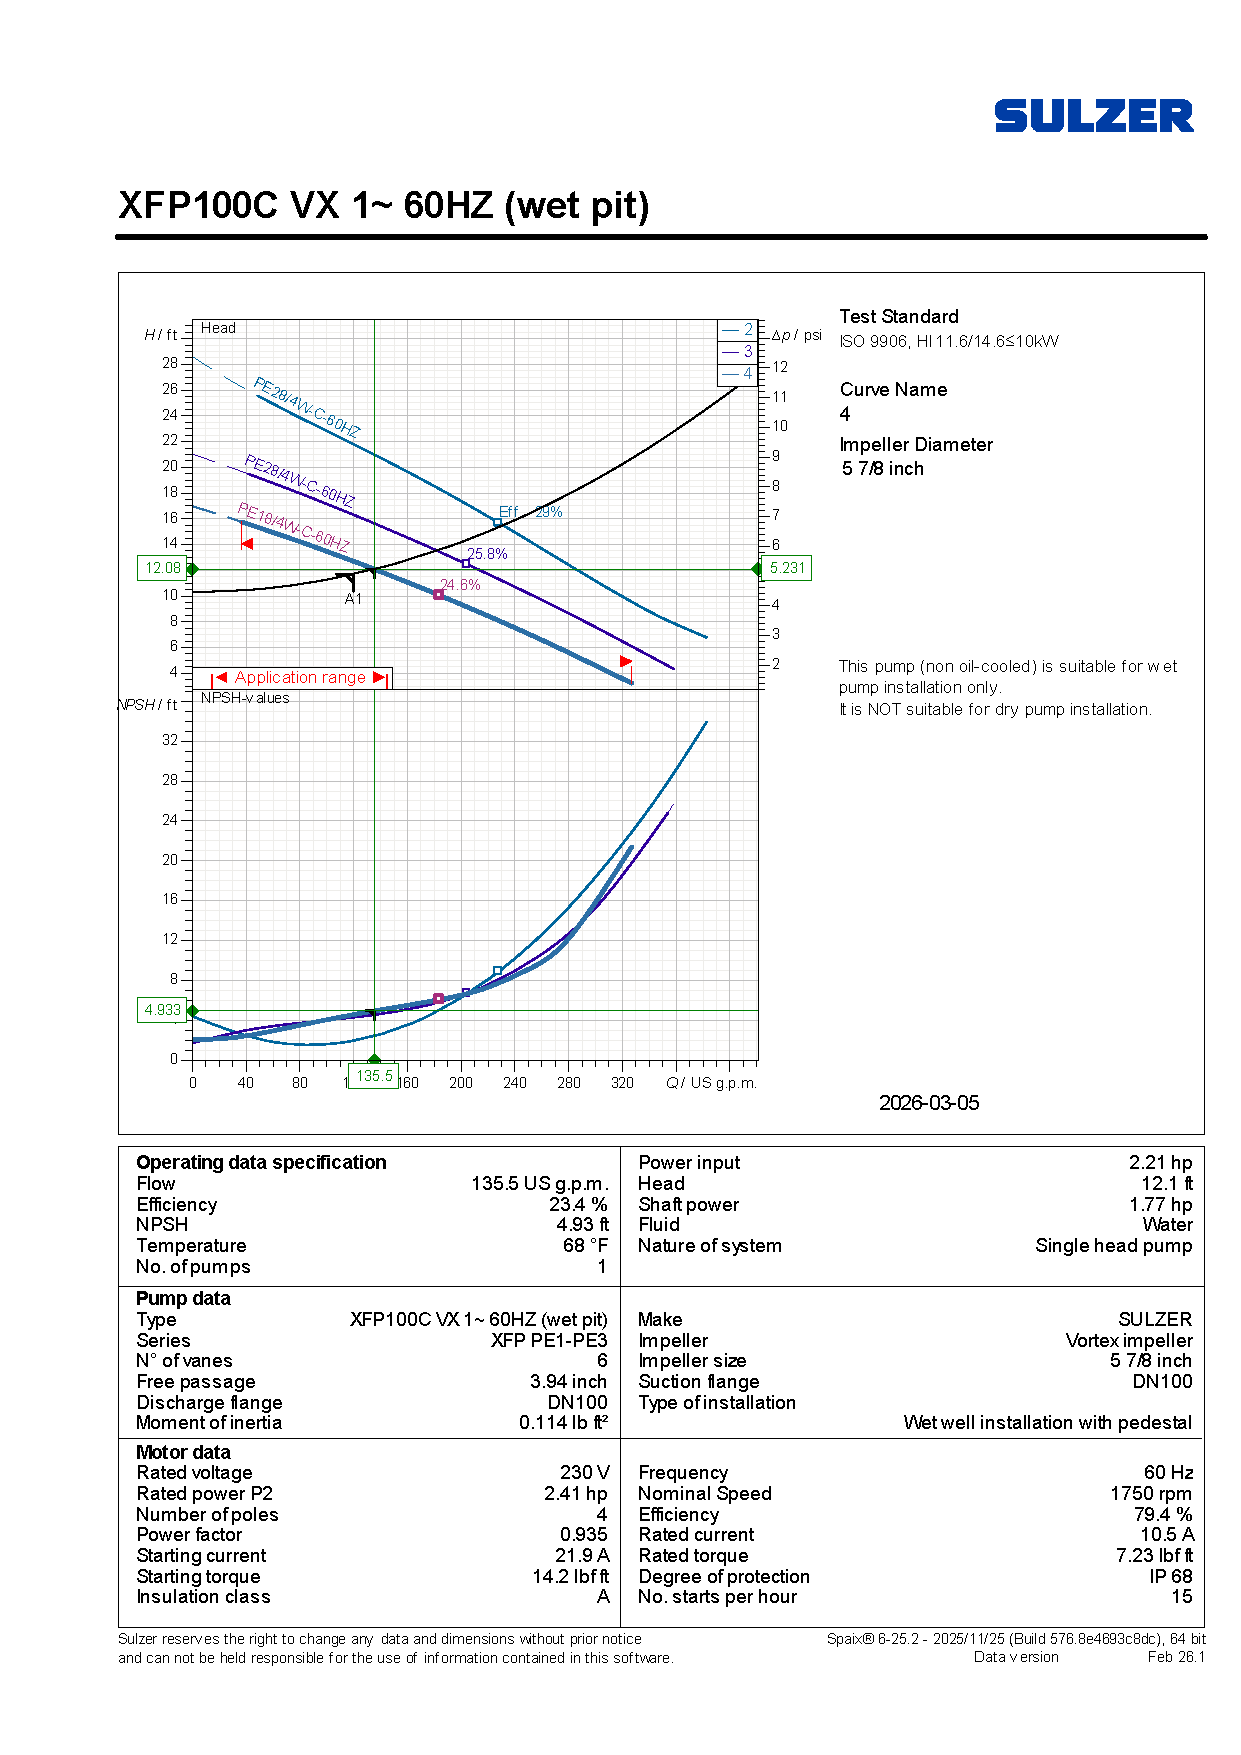
\includegraphics[
width=0.95\textwidth,
page=1,
]{./sulzer_xfp100c_curve.pdf}
\end{figure}

\includepdf[pages={2,3},pagecommand={},scale=0.9]{./sulzer_xfp100c_curve.pdf}


\section{XFP100C VX1 Dimension Sheet}
\begin{figure}[H]
\centering
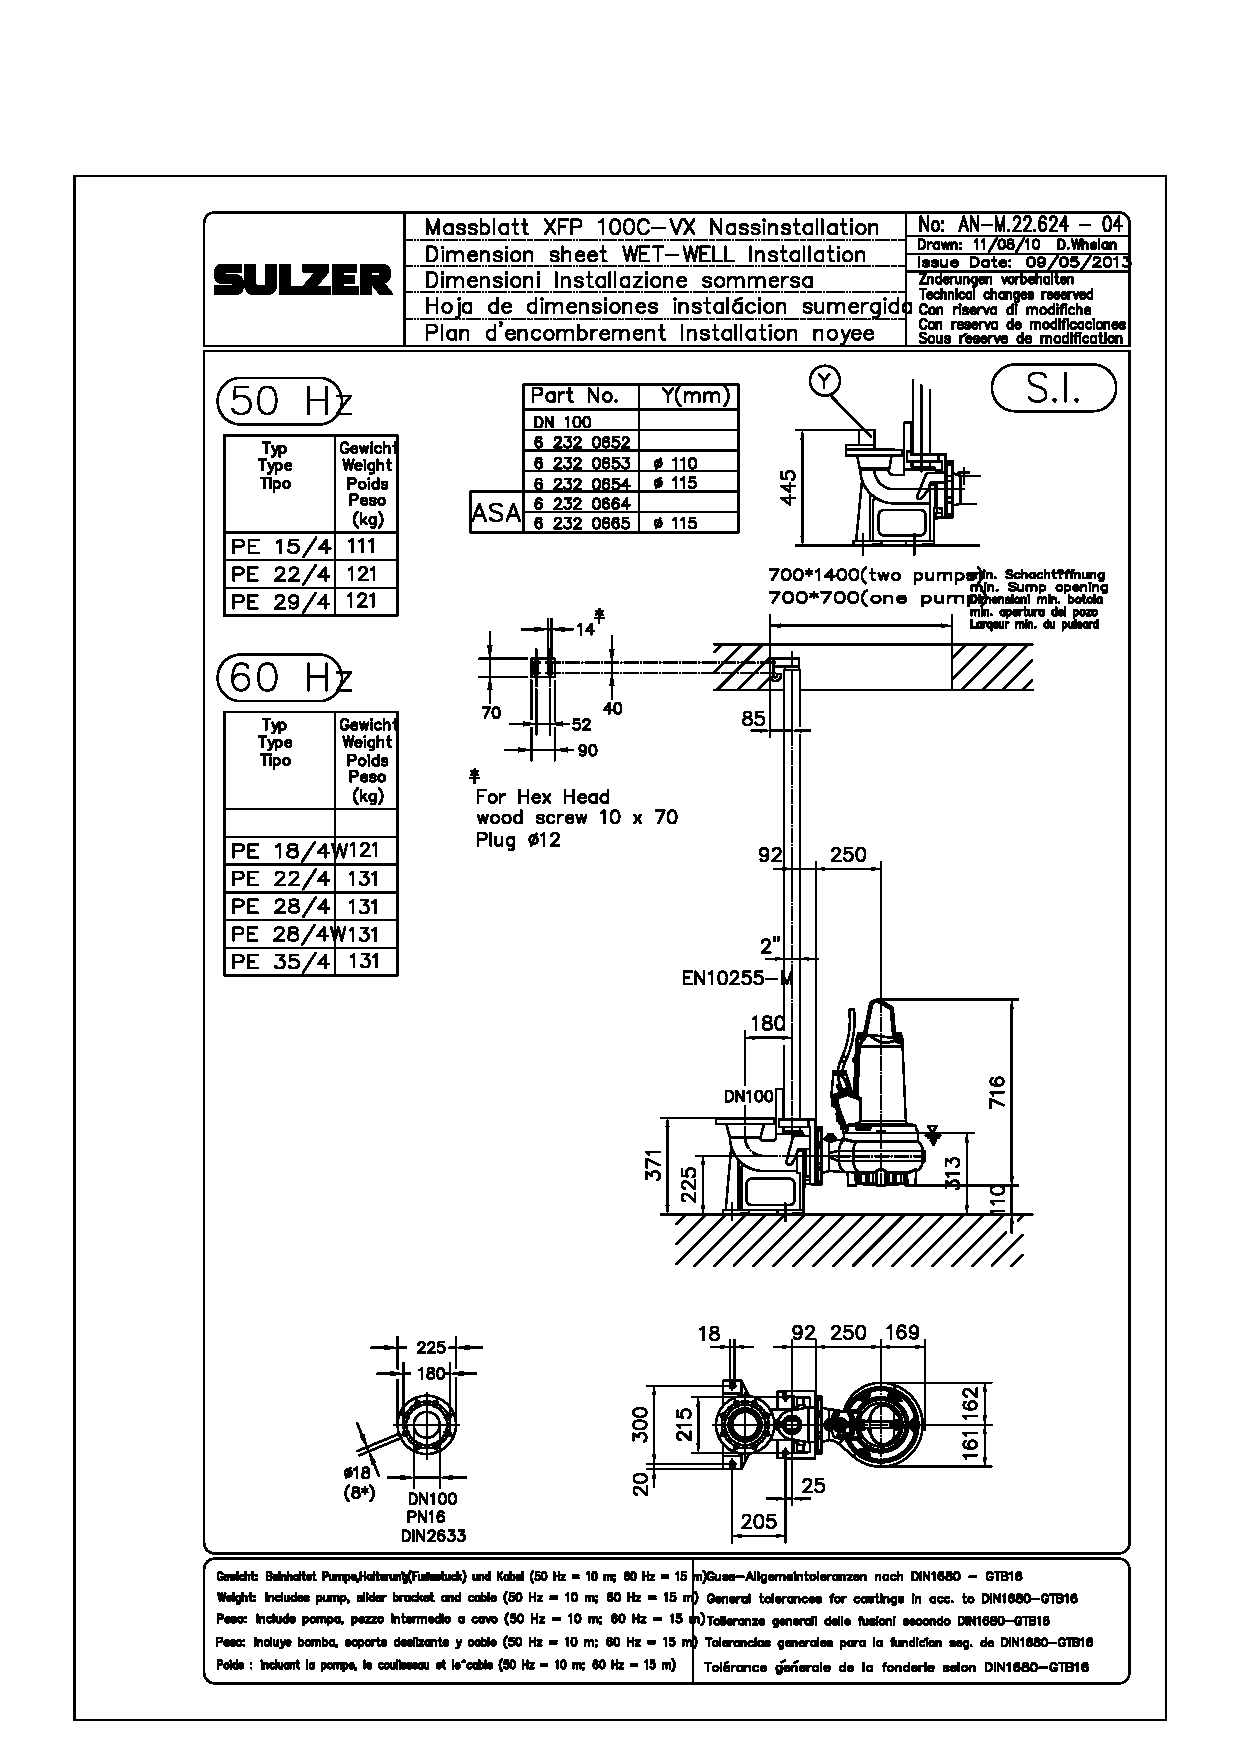
\includegraphics[
width=0.8\textwidth,
page=1,
]{./dimension_ANM22624.pdf}
\end{figure}

\begin{figure}[H]
\centering
\includegraphics[
width=0.95\textwidth,
page=2,
]{./dimension_ANM22624.pdf}
\end{figure}


% Appendix C
\renewcommand{\thesection}{C.\arabic{section}}
\setcounter{section}{0}
\setcounter{figure}{0}
\setcounter{table}{0}
\renewcommand{\thefigure}{C.\arabic{figure}}
\renewcommand{\thetable}{C.\arabic{table}}

\section{Detailed Cost Estimate Tables}

This appendix presents the detailed cost estimate used for the wastewater lift station and force main system. Table~\ref{tab:appendix_cost_detail} consolidates the direct construction costs, indirect costs, and engineering and design costs into a single detailed appendix table. Tables~\ref{tab:appendix_adders} and \ref{tab:appendix_total_cost} present the contractor adders and total project cost summary, respectively.

\begin{table}[H]
\centering
\caption{Detailed Cost Estimate}
\label{tab:appendix_cost_detail}
\begin{adjustbox}{width=\textwidth}
\begin{tabular}{c l c c c c}
\toprule
\textbf{Item No.} & \textbf{Description} & \textbf{Qty} & \textbf{Unit} & \textbf{Unit Cost (\$)} & \textbf{Line Cost (\$)} \\
\midrule
\multicolumn{6}{l}{\textbf{Direct Construction Costs}} \\
\midrule
1  & Sulzer XFP100C VX pumps & 2 & EA & 6,881.22 & 13,762.44 \\
2  & Precast concrete wet well (6-ft dia, 18--20 ft depth) & 1 & LS & 55,000.00 & 55,000.00 \\
3  & Valve vault and discharge assembly & 1 & LS & 22,000.00 & 22,000.00 \\
4  & Discharge piping system, guide rails, fittings & 1 & LS & 14,000.00 & 14,000.00 \\
5  & Check valve and gate valve (4-in) & 1 & LS & 6,500.00 & 6,500.00 \\
6  & Electrical and control system & 1 & LS & 38,000.00 & 38,000.00 \\
7  & Wet well protective coating & 1 & LS & 8,000.00 & 8,000.00 \\
8  & Site excavation, backfill, grading & 1 & LS & 22,000.00 & 22,000.00 \\
9  & Access pad / gravel surface & 1 & LS & 8,000.00 & 8,000.00 \\
10 & Erosion and sediment control & 1 & LS & 4,000.00 & 4,000.00 \\
11 & Quick-connect bypass assembly & 1 & LS & 5,500.00 & 5,500.00 \\
12 & 4-in PVC C900 DR18 force main & 80 & LF & 40.00 & 3,200.00 \\
13 & Trench bedding, backfill, restoration & 80 & LF & 20.00 & 1,600.00 \\
14 & Force main fittings, tracer wire & 1 & LS & 3,500.00 & 3,500.00 \\
15 & Connection to existing manhole & 1 & LS & 2,500.00 & 2,500.00 \\
16 & Traffic control & 1 & LS & 2,500.00 & 2,500.00 \\
\midrule
\multicolumn{5}{r}{\textbf{Direct Cost Subtotal}} & \textbf{210,062.44} \\
\midrule
\multicolumn{6}{l}{\textbf{Indirect Costs}} \\
\midrule
17 & Site preparation & 1 & LS & 6,000.00 & 6,000.00 \\
18 & Temporary facilities & 1 & LS & 4,000.00 & 4,000.00 \\
19 & Utilities allowance & 1 & LS & 3,500.00 & 3,500.00 \\
20 & Mobilization / demobilization & 1 & LS & 15,000.00 & 15,000.00 \\
\midrule
\multicolumn{5}{r}{\textbf{Indirect Cost Subtotal}} & \textbf{28,500.00} \\
\midrule
\multicolumn{6}{l}{\textbf{Engineering and Design Costs}} \\
\midrule
21 & Surveying & 1 & LS & 4,000.00 & 4,000.00 \\
22 & Geotechnical investigation & 1 & LS & 6,000.00 & 6,000.00 \\
23 & Design and consulting fees & 1 & LS & 18,000.00 & 18,000.00 \\
\midrule
\multicolumn{5}{r}{\textbf{Engineering \& Design Subtotal}} & \textbf{28,000.00} \\
\bottomrule
\end{tabular}
\end{adjustbox}
\end{table}

\begin{table}[H]
\centering
\caption{Cost Adders: Overhead, Profit, and Contingency}
\label{tab:appendix_adders}
\begin{tabular}{l c c c}
\toprule
\textbf{Category} & \textbf{Basis} & \textbf{Rate} & \textbf{Amount (\$)} \\
\midrule
Contractor Overhead & Direct + Indirect & 7\%  & 16,699.37 \\
Contractor Profit   & Direct + Indirect & 7\%  & 16,699.37 \\
Contingency         & Direct + Indirect & 10\% & 23,856.24 \\
\bottomrule
\end{tabular}
\end{table}

\begin{table}[H]
\centering
\caption{Total Project Cost Summary}
\label{tab:appendix_total_cost}
\begin{tabular}{l c}
\toprule
\textbf{Category} & \textbf{Amount (\$)} \\
\midrule
Direct Construction Costs & 210,062.44 \\
Indirect Costs            & 28,500.00  \\
Engineering \& Design     & 28,000.00  \\
Contractor Overhead       & 16,699.37  \\
Contractor Profit         & 16,699.37  \\
Contingency               & 23,856.24  \\
\midrule
\textbf{Total Project Cost} & \textbf{323,817.43} \\
\bottomrule
\end{tabular}
\end{table}



% \section*{Appendix A: TLDR}
% \section*{Flow Determination Procedure (Pump Station \& Force Main Design)}
% % Appendix B
% \section*{Appendix B: Preliminary Subdivision Plat}
% \addcontentsline{toc}{section}{Appendix B: Preliminary Subdivision Plat}
% \includepdf[pages=-,pagecommand={},scale=0.95]{\detokenize{subdivision_plat_Prelim Plat_Colebrooke Subdivsion (1) (1).pdf}}


\end{document}
